\documentclass[a4paper,12pt,onside]{report}

\usepackage{enumitem}
\usepackage{graphicx}
\usepackage{float}
\usepackage{xcolor}
\usepackage{cancel}
\usepackage{amsmath}
\usepackage{amssymb}
\usepackage{svg}
\usepackage{accents}
\usepackage{mwe} % For dummy images
\usepackage{wrapfig}
\usepackage{fancyhdr} 
\usepackage{comment}
\usepackage{rotating}
\usepackage{pdflscape}
\usepackage{setspace}
\usepackage{chemformula}
\usepackage{gensymb}
\usepackage{pdfpages}
\usepackage{textgreek}
\usepackage{caption}

\usepackage[Bjarne]{fncychap}
\usepackage{fullpage}
\usepackage{algorithm}

\usepackage[sectionbib]{natbib}
\usepackage{hanging}

\makeatother
\usepackage[utf8]{inputenc}
\usepackage{graphics}
\usepackage[graphicx]{realboxes}
\usepackage{subfigure} 

\usepackage{etoolbox}
\renewcommand{\bibname}{}
\usepackage{natbib}
\usepackage[hidelinks, backref]{hyperref}
\usepackage[top=2cm,bottom=4cm,outer=3cm,inner=3cm]{geometry}
\usepackage[hang,flushmargin]{footmisc}

\usepackage{cleveref}
\usepackage{appendix}
\usepackage{setspace}
\usepackage[super]{nth}
\usepackage{arydshln}
\usepackage{environ}

\usepackage[subfigure, titles]{tocloft}
\setlength{\cftsecnumwidth}{4em} % Set numwidth of section
\setlength{\cftsubsecnumwidth}{\cftsecnumwidth}% Make subsection numwidth the same as section
\setlength{\cftsubsecindent}{\cftsecindent}
\setlength{\cftsubsubsecindent}{\cftsecindent}
\setlength{\cftfignumwidth}{\cftsecnumwidth}
\setlength{\cfttabnumwidth}{\cftsecnumwidth} % Constant spacing 

\makeatletter
\newenvironment{chapquote}[2][2em]
  {\setlength{\@tempdima}{#1}%
   \def\chapquote@author{#2}%
   \parshape 1 \@tempdima \dimexpr\textwidth-2\@tempdima\relax%
   \itshape}
  {\par\normalfont\hfill--\ \chapquote@author\hspace*{\@tempdima}\par\bigskip}
\makeatother

\makeatletter
\setlength{\@fptop}{0pt}
\makeatother

\usepackage[font=small,labelfont=bf]{caption}
\setlength{\parindent}{15pt}

\setcounter{secnumdepth}{3}
\setcounter{tocdepth}{3}
\pagenumbering{roman}
\usepackage{acro}

%Term definitions
\DeclareAcronym{pa}{short=PA,long=Paris Agreement}
\DeclareAcronym{oae}{short=OAE,long=Ocean Alkalinity Enhancement}
\DeclareAcronym{cdr}{short=CDR,long=Carbon Dioxide Removal}
\DeclareAcronym{rf}{short=RF,long=Revelle factor}
\DeclareAcronym{esm}{short=ESM,long=Earth System Model}
\DeclareAcronym{om}{short=OM,long=organic matter}
\DeclareAcronym{mld}{short=MLD,long=mixed layer depth}
\DeclareAcronym{pp}{short=PP,long=primary producers}
\DeclareAcronym{dic}{short=DIC,long=Dissolved Inorganic Carbon}
\DeclareAcronym{foci}{short=FOCI,long=Flexible Ocean and Climate Infrastructure}
\DeclareAcronym{mops}{short=MOPS,long=Model of Oceanic Pelagic Stoichiometry}
\DeclareAcronym{ipcc}{short=IPCC,long=Intergovernmental Panel on Climate Change}
\DeclareAcronym{ghg}{short=GHG,long=greenhouse gases}
\DeclareAcronym{ssp}{short=SSP,long=socio-economic pathway}
\DeclareAcronym{sst}{short=SST,long=sea surface temperature}
\DeclareAcronym{ir}{short=IR,long=Industrial Revolution}

\begin{document}

\newcounter{rom}

\begin{titlepage}
\centering
\vspace*{\fill}
\begin{Large}\bfseries

\textsc{Impacts of Ocean Alkalinity Enhancement on the Seasonal Cycle of \ch{CO2} Flux and Ocean \ch{pCO2} in European Waters}

\end{Large}
%\vspace{0.25cm}
%\begin{Large} \bfseries
%The Organisation and Influence of Business Interests in %Policy-Making Processes\par
%\end{Large}
\vspace{3cm}

\begin{center}%
M.Sc. Thesis Dissertation \\ \vspace{0.25cm}
Student number 1126202 \\ \vspace{0.25cm}
Course code WSG80400 \\ \vspace{0.25cm}
Study programme Climate studies \\ \vspace{0.25cm}
\vspace{2.5cm} 
Author \\\vspace{0.15cm}
\vspace{0.15cm} 
Chiara Ciscato \\ \vspace{0.25cm}
\vspace{1cm} 
\vspace*{\fill}
Wageningen University \& Research \\ \vspace{0.25cm}
Wageningen, The Netherlands \\ \vspace{0.25cm}
\today \\ \vspace{0.25cm}
\end{center}
\end{titlepage}\newpage\thispagestyle{plain}
\vspace*{\fill}
\begin{tabular}{ll}
    Supervisor at GEOMAR: & Dr. David P. Keller\\
    Supervisor at WUR: & Dr. Ronald Hutjes\\
\end{tabular}

\newpage
\textbf{Disclaimer}

\vspace{0.2in}

This report is produced by a student of Wageningen University as part of his or her MSc-programme. It is not an official publication of Wageningen University and Research, and the content herein does not represent any formal position or representation by Wageningen University and Research.

\newpage
\begin{abstract}

Anthropogenic climate change is induced by, among other causes, the release of heat-trapping \ch{CO2} into the atmosphere from fossil fuel burning. According to the Intergovernmental Panel on Climate Change, in order to meet the target set by the Paris Agreement, emission reduction must be complemented by Carbon Dioxide Removal technologies aiming to sequester \ch{CO2} from the atmosphere and store it in natural reservoirs. One of such methods is Ocean Alkalinity Enhancement (OAE), which aims to lower ocean \ch{CO2} partial pressure (\ch{pCO2}) and accelerate the natural \ch{CO2} uptake through chemical weathering. As seasonality is a fundamental component of the ocean net annual \ch{CO2} uptake, this study aims to bridge the knowledge gap on the impacts of OAE on the seasonal cycle of \ch{CO2} flux and ocean \ch{pCO2}. An analysis was conducted on two Earth System Model outputs simulating alkalinity addition along the European coastline (with the exception of the Baltic and the Mediterranean seas), for both a low and a high emission scenario (SSP1-2.6 and SSP3-7.0, respectively). It was found that: the \ch{CO2} seasonal flux is amplified with alkalinity addition, especially in winter, likely as a consequence of a larger imbalance at the air-sea interface; the ocean \ch{pCO2} seasonal cycle is dampened, especially in summer, due to its decreased sensitivity to \ch{CO2} fluctuations in an alkalinised ocean; both effects are magnified under SSP3-7.0. This suggests that OAE induces asymmetrical impacts on \ch{CO2} seasonality, with potentially significant alterations to the net annual cycle. 

\end{abstract}

%\newpage\thispagestyle{plain}

%\newpage\thispagestyle{plain}\setcounter{page}{3}

\tableofcontents
\listoffigures
\listoftables
\printacronyms

\newpage\thispagestyle{plain}~
\cleardoublepage
\pagenumbering{arabic}

\onehalfspacing

\chapter{Introduction:}

Anthropogenic climate change is the product of human activities \citep{trenberth2018climate} that have been implemented since the \ac{ir} and that have strongly intensified in recent decades. Among other effects, global warming results from the increasing concentration of heat-trapping \ac{ghg} in the atmosphere mainly due to fossil fuel burning, which causes global temperatures to rise. This and other climatic alterations heavily affect local communities and natural ecosystems around the world, leading to "severe, pervasive and irreversible impacts" \citep{change2014impacts}.

According to most projections, the \ac{pa} to keep global temperatures well below 2\textdegree C, and possibly below 1.5\textdegree C, compared to pre-industrial levels, is unlikely to be realised by the end of the century only by reducing \ac{ghg} emissions. In fact, most model predictions show that existing commitments are inadequate to meet such targets \citep{lawrence2018evaluating}. The \ac{ipcc} report drawn up by the Working Group III reinforces this evidence by stating that national unconditional commitments determine a global warming far beyond \ac{pa} standards and that human manipulation of the earth’s climate is necessary to offset hard-to-abate emissions \citep{IPCC_2022_WGIII_SPM}.

As \ch{CO2} is one of the most potent \ac{ghg} contributing to the earth's warming, \ac{cdr} is being investigated as part of the \ac{pa}-driven collaborative mission to achieve climate mitigation. The aim of this technique is to relieve the atmosphere from \ch{CO2}-induced pollution and reach net negative emissions by 2100. Therefore, this research focuses on an example of marine \ac{cdr}, that is, carbon dioxide sequestration and storage in oceanic reservoirs, termed \ac{oae}. This method aims to enhance surface ocean alkalinity through accelerated chemical weathering of mineral rocks or solutions in order to reduce ocean \ch{CO2} partial pressure (\ch{pCO2}) and increase the ocean's uptake potential. 

For this manuscript, output data from two \ac{esm} simulations were analysed, projecting future scenarios with and without alkalinity applied to the European coastline (excluding the Baltic and the Mediterranean seas) for a low and a high emission scenario (SSP1-2.6 and SSP3-7.0, respectively). The purpose was to understand the effects of \ac{oae} on the carbon cycle and, particularly, on its seasonal variations, as seasonality is a fundamental component regulating the annual net carbon flow at the air-sea interface.

This paper develops as follows. First, the study objectives and hypotheses are formulated. The second chapter aims to illustrate the present-day relevance of marine \ac{cdr}, and especially of \ac{oae}, and describe the factors that drive \ch{CO2} flux and ocean \ch{pCO2} seasonality, both globally and in the study area. In the third chapter, the methods are presented, giving a description of the \ac{esm} and of the simulations utilised for this manuscript, together with a brief overview of the addressed variables. The results are provided in the fourth chapter. The fifth chapter includes a discussion section, which outlines the possible causes behind the findings, and the sixth highlights the study's limitations and some key recommendations for future research. 

\section{Study objectives and hypothesis formulation:}

As the \ac{pa} targets become increasingly difficult to attain, the employment of \ac{cdr} to counterbalance hard-to-abate emissions is considered a future necessity \citep{IPCC_2022_WGIII_SPM, shukla2022summary}. Despite being a potentially significant contribution to climate mitigation, \ac{oae}, one of the proposed marine-\ac{cdr}, is still widely unexplored \citep{fakhraee2022environmental}. Thus, more research is needed to shed light on the impacts of \ac{oae} on the cycle of \ch{CO2} and ocean \ch{pCO2} at the air-sea interface. This is the case especially for coastline alkalinity addition, where such highly dynamic environments are thought to be particularly favourable to accelerated carbon sequestration \citep{he2022limits, thomas2009enhanced}. 

Seasonality is one of the fundamental elements influencing the net annual \ch{CO2} cycle. Understanding how such patterns will evolve with large-scale \ac{oae} implementation is therefore relevant for a variety of reasons. First, if changes to the seasonal carbon cycle are not counterbalanced by compensating effects in the opposite direction, these asymmetries may trigger significant modifications to the annual net cycle \citep{fassbender2022quantifying}. Furthermore, \ch{CO2} flux seasonality is a central driver of ocean extreme events such as earlier calcium carbonate undersaturation \citep{kwiatkowski2022modified} and intensified ocean acidification \citep{sasse2015quantifying}, other than acting upon inter-annual variability patterns \citep{rustogi2023impact}. Lastly, while atmospheric \ch{pCO2} responds to system stimuli at much shorter timescales, the ocean can take several seasons to react \citep{salt2013variability} and defining such time lapses is necessary for future \ac{oae} application.

Thus, up to this day, uncertainty remains on how \ac{oae} would affect \ch{CO2} seasonality and what patterns it would follow under different future climatic conditions. The main research questions that were formulated to address this knowledge gap are:
\begin{enumerate}

  \item How will \ac{oae} modify the \ch{CO2} flux and ocean \ch{pCO2} seasonal cycle in European waters?
  \item What are the main physical and biological drivers of such system alterations?
  \item What role does the future emission scenario play in the seasonality of \ch{CO2} flux and ocean \ch{pCO2} when \ac{oae} is implemented?
  
\end{enumerate}

A 2022 report by \citeauthor{schwinger2022report} pictured an idealised simulation of global \ac{oae} application to account for seasonal implications of \ch{CO2} flux and other variables. Results showed that \ac{oae} has the potential to increase the \ch{CO2} seasonal cycle, elicited by the ocean's enhanced buffering capacity and, to a lesser extent, temperature growth. In addition, ocean \ch{pCO2} seasonal amplitude was projected to decrease as a consequence of its reduced sensitivity to \ac{dic} modulations \citep{schwinger2022report}. Following such premises, it was hypothesised that the \ch{CO2} seasonal flux would be enhanced with alkalinity addition whereas ocean \ch{pCO2} seasonality would be dampened. 

\chapter{Context:} 

\section{\ac{cdr}:}

\acl{cdr} technologies aim to reduce \ch{CO2} concentration in the atmosphere through two pathways. On the one hand, carbon dioxide can be extracted directly from the air and stored in permanent natural reservoirs. An example is direct air capture with \ch{CO2} storage, which entails the absorption and injection of atmospheric \ch{CO2} in geological or marine reservoirs \citep{pires2011recent}. On the other hand, the carbon storing capacity of the land and the ocean, which each already take up about a third of annual emitted anthropogenic \ch{CO2}, can be enhanced \citep{keller2018effects}. An example is \ac{oae}, a marine \ac{cdr} option with theorised large-scale potential.

\ac{cdr} raises strong debate in the scientific community, as none of the aforementioned methods has yet been applied large-scale, and environmental burdens and potential drawbacks have not been investigated thoroughly \citep{terlouw2021life}. There are, for example, uncertainties on the socio-economic feasibility of \ac{cdr}, mainly related to the high energy requirements, which could offset much of the \ch{CO2} sequestration potential \citep{kheshgi1995sequestering}. The ethics behind climate manipulation is also questioned. A 2013 study defined such technologies a "moral hazard" that risk to shift the global focus away from emission reduction efforts \citep{preston2013ethics} and trigger free-riding mechanisms. Transparent research and comprehensive frameworks are therefore being developed to govern this new field and avoid undermining the collective effort towards climate mitigation \citep{honegger2021paying}.

Marine \ac{cdr} involves the employment of wetlands, bank shelves and the open ocean for carbon dioxide sequestration and storage, and recently gained international attention as the blue frontier for human intervention on the earth's climate \citep{boettcher2021navigating}. Some of the investigated marine \ac{cdr} options are: removing \ch{CO2} from seawater and storing it in nonmarine or geological reservoirs; enhancing carbon storage in biomass, detritus and dissolved organic carbon pools; injecting \ch{CO2} directly into the deep ocean; artificially upwelling nutrient-rich waters to the ocean surface to encourage the activity of \ac{pp}; increasing ocean alkalinity, and hence the ocean buffering capacity, to maximise its uptake potential \citep{NAP26278}. The reason for focusing on the ocean as an efficient carbon reservoir has to do with its major role in the global carbon cycle.

\section{The role of the ocean in the carbon cycle:}

\subsection{Ocean biogeochemistry:}

The ocean forms about 70\% of the earth's surface and 95\% of its biosphere, hence representing a major component in the global carbon cycle \citep{ma2015primary}. Through a variety of physical, chemical, and biological processes, the ocean constitutes a net sink of atmospheric \ch{CO2} and stores about 40,000 Gt of carbon in its interior and deep waters \citep{wang2023simulated}. For comparison, the soils, vegetation and permafrost altogether hold less than 4,000 Gt of carbon. 

Since the beginning of the \ac{ir}, the ocean has absorbed about 90\% of the excess heat \citep{butenschon2021alkalinization} and about 26\% of total \ch{CO2} anthropogenic emissions, amounting to 2.9 GtC yr\textsuperscript{-1} \citep{friedlingstein2022global}. This is an estimate that has remained remarkably stable in the last decades and that represents a valuable resource for climate stabilisation \citep{friedlingstein2022global, scott2019role}. Additionally, as the ocean represents the largest surface area, it constitutes the predominant, long-lasting carbon reservoir, of which immense quantities will eventually be stored for decades to millennia \citep{archer2009atmospheric}. 

Thanks to seawater solubility and chemical properties, the ocean can store much higher amounts of carbon compared to its counterparts, the land and the atmosphere. The \ac{dic} pool comprises the three speciations of aqueous \ch{CO2} (\ch{CO2(aq)}), bicarbonate (\ch{HCO3-}) and carbonate (\ch{CO3^{2-}}). Bicarbonate is by far the most abundant in seawater, accounting for about 90\% of the \ac{dic} pool, whereas 1\% and 10\% are the relative concentration of \ch{CO2(aq)} and \ch{CO3^{2-}}, respectively \citep{marchitto2007paleoceanography}. 

Carbon dioxide enters the ocean as \ch{CO2(aq)} and reacts with seawater (see \ref{eqn:2.1}), forming carbonic acids (\ch{H2CO3}). Carbonic acid readily dissociates into bicarbonate and releases one proton (\ch{H+}) (\ref{eqn:2.2}). Bicarbonate can then dissociate again to form carbonate, releasing another proton (\ref{eqn:2.3}). As pH describes the negative logarithmic concentration of hydrogen ions in a system, a positive relationship between ocean \ch{CO2} uptake and proton accumulation is clearly derived from these formulas, where carbonic acid dissociation induces the release of free protons and therefore lowers pH levels. 

\begin{center}

\begin{equation}
\label{eqn:2.1}
\ch{CO2(aq)} + \ch{H2O} \leftrightarrow \ch{H2CO3}
\end{equation}

\begin{equation} 
\label{eqn:2.2}
\ch{H2CO3} \leftrightarrow \ch{HCO3-} + \ch{H+}
\end{equation}

\begin{equation} 
\label{eqn:2.3}
\ch{HCO3-} \leftrightarrow \ch{CO3^{2-}} + \ch{H+}
\end{equation}

\end{center}

\ch{pCO2} expresses the \ch{CO2} partial pressure gradient between the air and the sea surface boundary, where \ch{CO2} exchange takes place, and it is a key element to understand the atmosphere-to-ocean relations. As atmospheric \ch{CO2} concentration rises with increasing emissions, air \ch{pCO2} also grows, and today, due to elevated \ac{ghg} emissions, it is increasing at the fastest rate in the past 65 million years \citep{watson2017quantifying}. 

Since the beginning of the \ac{ir}, ocean \ch{pCO2} has been growing at a smaller rate than atmospheric \ch{pCO2}, forcing the flow of \ch{CO2} into the ocean \citep{lenton2012observed}. However, the relation between the two remains constant, and more atmospheric \ch{CO2} concentrations will automatically lead to enhanced ocean uptake, although at a lower rate due to its reduced buffering capacity \citep{chikamoto2023long}. Ocean \ch{pCO2} is influenced by a multitude of biological and physical factors, among which are \ac{sst}, pH, primary production and ocean mixing \citep{fassbender2022quantifying, kheshgi1995sequestering}. 

\subsection{The ocean's carbon pumps:}

The partitioning of the three carbon species listed above, the \ch{CO2} transfer between the atmosphere and the ocean surface, and the changes in vertical distribution are controlled by two pumps: the solubility pump \citep{heinze2015ocean}, which is the dominant process for \ch{CO2} transport to the deep, and the biological pump, which is responsible for maintaining the carbon gradient along the water column. Both pumps act against the natural carbon distribution gradient and their activity is connected to the ocean division into two layers defined by three physical properties: temperature, salinity, and, as a result of the previous two, density. The ocean surface, which represents the surface mixed layer, receives more insulation and is therefore warmer, with lower density and salinity levels. On the other hand, the deep ocean, which holds most of the ocean's \ac{dic}, is colder, denser and more saline. Due to stratification, these two regions do not interact easily, and strong mixing only happens within the mixed layer compartment. 

In the solubility pump, \ch{CO2} is carried to the deep ocean through sea currents that transport the carbon exchanged at the atmosphere-ocean interface. As gases are less soluble in warmer water, the colder, deeper ocean holds most of the \ac{dic}, which creates a marked gradient between equatorial and polar regions as well as between the upper and interior ocean. Carbon follows the movement of the water from lower latitudes towards the poles, where it gradually cools and favours the solubility of \ch{CO2}, replenishing the \ac{dic} pool. Here, colder, denser water downwells and deposits carbon at depth. This process takes place in the Southern Ocean and northern North Atlantic, where ice formation leaves dense brine to sink and favour deep water formation \citep{reid2009impacts}. 

When referring to the biological pump, a conceptual subdivision is needed: the soft-tissue pump refers to \ac{om} production and respiration, while the carbonate counter-pump is the combination of the two processes of carbonate formation and dissolution. The former is driven by the activity carried out by autothrops in the photic zone, where light penetrates and is available for photosynthesis. Part of the carbon assimilated through net primary production escapes respiration and is transported to the ocean interiors. In broad terms, this can happen through gravitational sinking of dead phytoplankton, the migration of animals below the photic zone, or physical mixing. The latter pump is performed by organisms that synthesise carbonate ions to produce their hard exoskeletons. Coccolithophores and corals are some of the species involved in the incorporation and dissolution of \ch{CaCO3} \citep{devries2022ocean}, therefore regulating one of the most fundamental ocean properties, that is, alkalinity.  

\subsection{Alkalinity:}

Alkalinity describes the excess of bases, or proton acceptors, over acids, or proton donors, and it is a conservative property of the ocean as it is not influenced by temperature and pressure changes \citep{wolf2007total}. When entering the ocean, \ch{CO2} acts as a proton donor that reacts with water to form bicarbonates (see \ref{eqn:2.2}) and carbonates (see \ref{eqn:2.3}), releasing hydrogen ions. Alkalinity then acts as a buffer to neutralise ocean acidity through the bonding with free \ch{H+} \citep{middelburg2020ocean}. This property is largely balanced by two opposing processes: the ions generated through rock weathering, which releases alkalinity (left of the arrow in \ref{alkrelease}), and the ions consumed through calcium carbonate formation, which consumes alkalinity and frees \ch{CO2} molecules (right of the arrow in \ref{alkrelease}). 

\begin{center}

\begin{equation} 
\label{alkrelease}
\ch{Ca}\textsuperscript{2+} +  2\ch{HCO3-} \leftrightarrow \ch{CaCO3} + \ch{CO2} + \ch{H2O}
\end{equation}

\end{center}

\section[\texorpdfstring{OAE}{OAE} as marine \texorpdfstring{CDR}{CDR}:]{\ac{oae} as marine \ac{cdr}:}

Different options are being investigated on how the ocean can play a role in further atmospheric \ch{CO2} uptake. One of them is enhanced chemical weathering, which involves the acceleration of the geological process whereby atmospheric \ch{CO2} is chemically consumed when reacting with rainwater on land, after which the product reaches the ocean mainly via runoff, or directly with seawater in the ocean. Although chemical erosion already happens naturally and will eventually sequester all anthropogenic \ch{CO2} emitted so far, it will take thousands of years for this process to complete \citep{archer2009atmospheric}. Hence, enhanced weathering aims to speed up the mechanism and contribute to lower global warming on a human-relevant timescale. 

The concept of enhanced weathering was first introduced by \cite{kheshgi1995sequestering}, who theorised the addition of the dissolution products of alkaline minerals to seawater, which would increase its buffering capacity and stimulate \ch{CO2} solubility. Enhanced weathering, like natural weathering, would then be partly compensated for by \ch{CaCO3} precipitation, mainly performed by calcifying organisms \citep{NAP26278}. 

Alkalinity addition can be performed in two ways. Alkaline-rich minerals can be pulverised and distributed directly onto terrestrial landscapes, in a process termed enhanced terrestrial weathering \citep{bach2019co2}, as it accelerates the on-land natural erosion of rocks through the chemical breakdown of silicates and carbonates with rainwater \citep{taylor2016enhanced}. During this process, stable bicarbonate and carbonate ions are produced and then carried to the ocean, mainly through land and riverine runoff. In the ocean, the mean residence time of these ions, which are sometimes slowly incorporated to deep-ocean rocks, is about 100,000 years, and can act as a permanent carbon storage on a human timescale \citep{renforth2017assessing}. Currently, natural terrestrial weathering is estimated to remove around 1 Gt yr\textsuperscript{-1} of \ch{CO2} \citep{zhang2022river}. 

\begin{figure}[H]
\caption[Visualisation of some \texorpdfstring{OAE}{OAE} implementation options]{Visualisation of some \ac{oae} implementation options}
\label{oae}
\centering
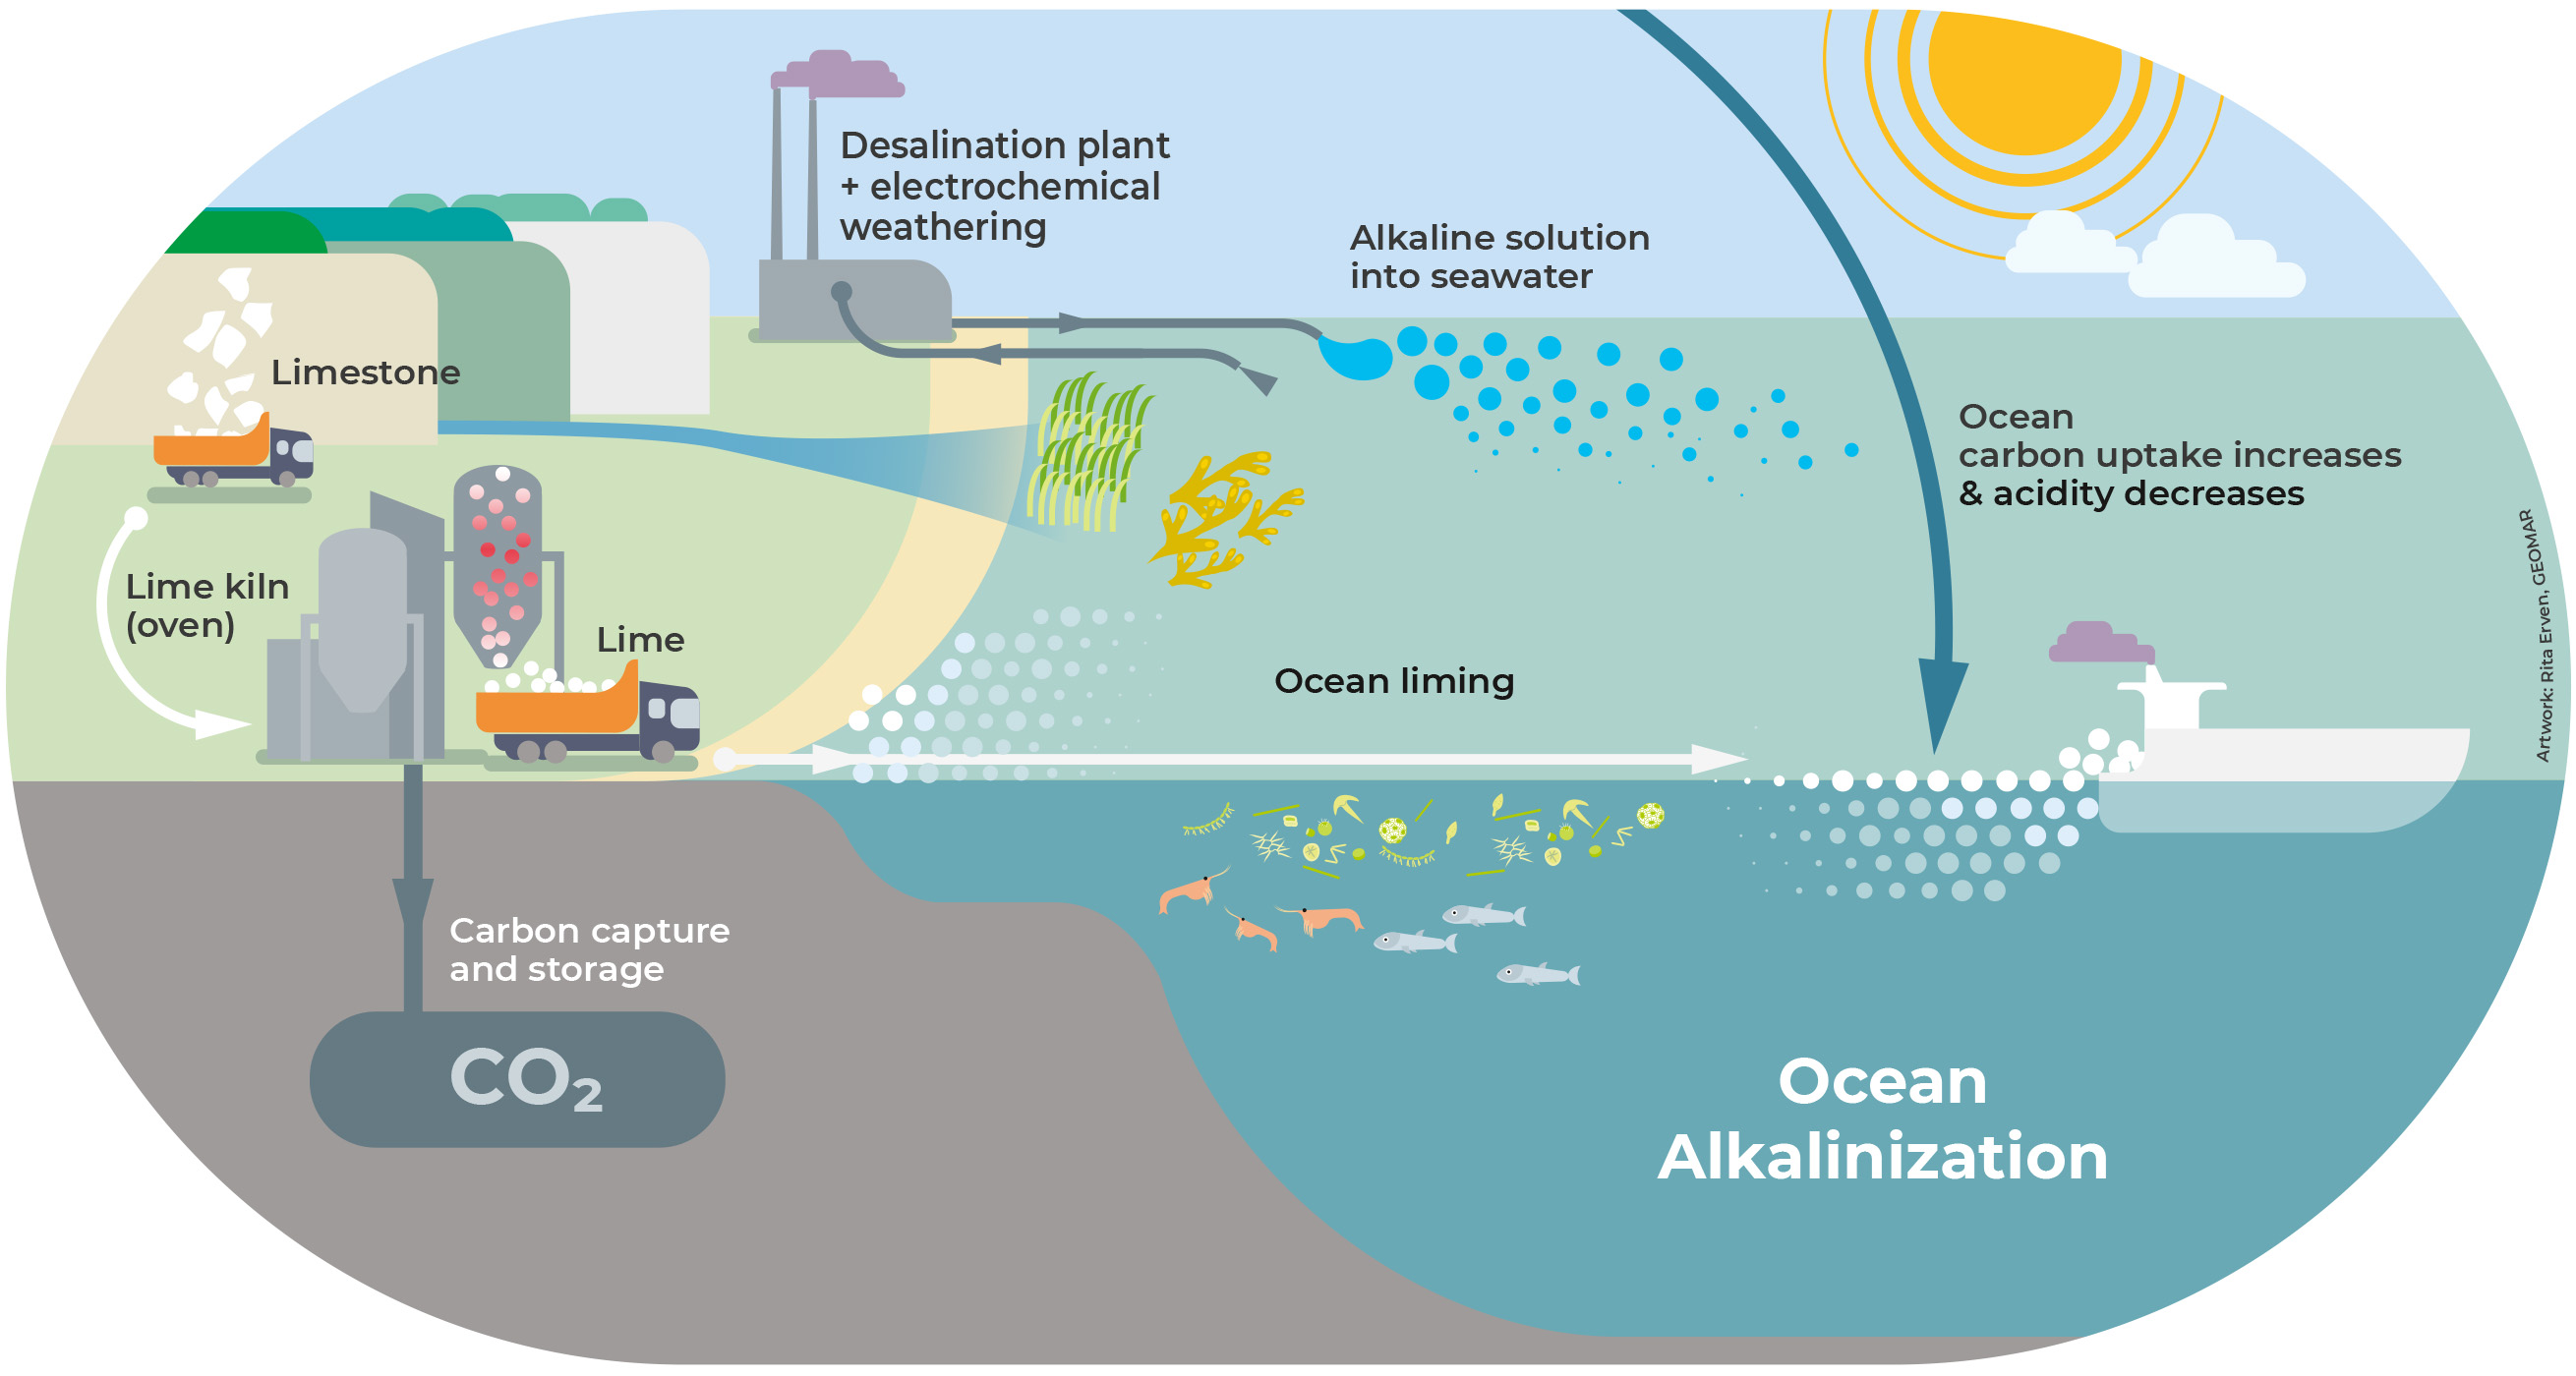
\includegraphics[width=12cm]{fig/1_Introduction/alkalinization_210325.jpg}

\scriptsize Source: Rita Ervin, GEOMAR
\end{figure}

The second method for alkalinity addition is through \acl{oae}, described in \cref{oae}. As atmospheric \ch{CO2} easily dissolves in seawater under the chemical reactions discussed above, \ac{oae} aims to reduce the fragment of aqueous \ch{CO2} present in seawater, which is constantly being exchanged with the atmosphere, and convert it into \ch{HCO3-} and \ch{CO3^{2-}}, thus promoting atmospheric \ch{CO2} drawdown. 

In general terms, \ac{oae} involves the dissolution of silicate and carbonate rocks and solutions, by either grinding and dispersal on the ocean surface, or by electro-chemical reaction on land-based stations or on board of ships. To mention a few, alkalinity can be generated through calcium carbonate dissolution, which produces carbonate ions (see \ref{split}) \citep{rau2008electrochemical}, or by converting salt present in seawater or desalination plants into a basic solution (see \ref{electrochem}) \citep{shaw2022understanding}. The product of such reactions, that is, alkalinised seawater, would then be returned to the ocean to increase its buffering capacity.

\begin{center}

\begin{equation}
\label{split}
\ch{CaCO3} \leftrightarrow \ch{Ca}\textsuperscript{2+} + \ch{CO3}\textsuperscript{2-}
\end{equation}

\begin{equation}
\label{electrochem}
\ch{NaCl} + \ch{H2O} \leftrightarrow \ch{HCl} + \ch{NaOH}
\end{equation}

\end{center}

At present day, natural ocean weathering already sequesters around 0.5 billion tonnes of \ch{CO2} every year \citep{NAP26278}.

\subsection[\texorpdfstring{OAE}{OAE}-induced impacts:]{\ac{oae}-induced impacts:}

\ac{oae} induces ocean \ch{pCO2} to decrease as seawater chemistry moves towards a carbonate-dominated system. This shift drives the \ac{dic} pool to be depleted in \ch{CO2}(aq), leading to more \ch{CO2} to flow from the atmosphere into the ocean to restore the air-sea equilibrium. Due to its properties, alkalinity addition is therefore strictly linked to the replenishment of the \ac{dic} pool \citep{he2022limits}.

\ch{CO2} uptake efficiency varies depending on the amount of alkalinity needed to drive such alterations. This principle is expressed by the \ac{rf}, which defines \ch{pCO2} sensitivity as a function of \ac{dic} variations. \ac{rf} is mathematically translated as the relative change in \ch{pCO2} divided by the relative change in \ac{dic} \citep{devries2022ocean} and it is inversely proportional to the ocean's buffering capacity \citep{renforth2017assessing}. Higher (lower) \ac{rf} implies that smaller (larger) \ac{dic} modulations are needed to produce the same ocean \ch{pCO2} response. It has been estimated that, in a global range between 8 and 15, \ac{rf} has risen by one unit since pre-industrial levels \citep{mcneil2019changing, egleston2010revelle}.

As \ac{oae} aims to enlarge the air-to-sea \ch{CO2} disequilibrium, it is worth highlighting the main properties that regulate the requilibration timescale which, as cited in \cite{jones2014spatial}, is seasonally and location dependent, varying from a few months to over a year. Generally speaking, the \ch{CO2} requilibration rate ($\tau$\ch{CO2}) is determined by four factors (\ref{equilrates}): 

\begin{center}

\begin{equation} 
\label{equilrates}
\tau \ch{CO2} = hR/GB
\end{equation}

\end{center}

where h is the \ac{mld}, R is the \ch{CO2}(aq):\ac{dic} ratio, G is the gas transfer velocity, and B is the \acl{rf}. From this equation, it is derived that locations with shallower \ac{mld} will allow for faster requilibration, given its linear relation with the \ch{CO2}(aq) content. G is driven by, among others, wind-induced turbulence, and areas exposed to high wind speed will experience faster requilibration. At the same time, however, wind speed deepens the \ac{mld} and slows down the exchange rate, so that the dominating process will drive the transfer rate. Whereas R usually decreases with latitude, B has the opposite trend and, inversely correlated with $\tau$\ch{CO2}, shortens the gas exchange rate \citep{jones2014spatial}. 

\ac{oae} has the additional benefit of alleviating the ocean from increasing acidification, a present-day threat that relates to rising \ch{H+} concentration in seawater as a consequence of \ch{CO2} downward inputs \citep{ma2015primary}. Since the start of the \ac{ir}, ocean pH has declined by 0.1 units \citep{devries2022ocean}, leading to widespread impacts on the ocean biota such as major coral bleaching events and reduced biodiversity.

\begin{figure}[H]
\caption{Relation between ocean carbon chemistry and pH}
\label{pHacid}
\centering
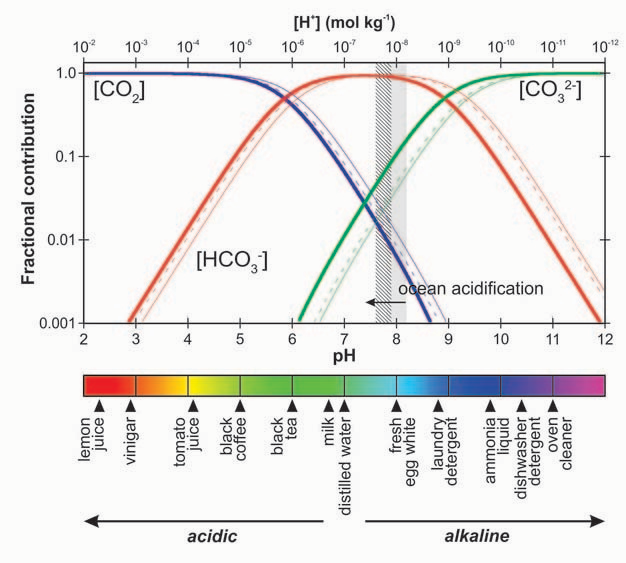
\includegraphics[width=10cm]{fig/1_Introduction/Carbonate_Chemistry.png}

\scriptsize Source: \cite{barker2012ocean}
\end{figure}

\Cref{pHacid} represents the relation between pH and ocean chemistry. Each coloured line describes the concentration of the three forms of carbon as a function of pH. At higher pH, possibly induced by \ac{oae}, the system moves towards a carbonate-dominated environment (green line in \Cref{pHacid}), where more carbonate ions are available and aqueous \ch{CO2} content drops. Moving towards the left-hand side of the graph, when pH lowers, carbon present in the form of \ch{CO2}(aq) grows, whereas the concentration of its stable forms decreases.

pH is partly affected by the biological carbonate counter-pump, which regulates the formation and dissolution of \ch{CaCO3}. pH neutralisation happens when, as a surplus quantity of \ch{CO2} enters the system, carbonate ions bond with extra \ch{H+} to form bicarbonates and reduce acidity \citep{scott2019role, barker2012ocean}. At the same time, however, \ch{CO3^{2-}} that combines with calcium (\ch{Ca}\textsuperscript{2+}) to build the exoskeletons of marine calcifiers, starts dissolving to favour bicarbonate production \citep{mcnicholl2020ocean}.

\subsection[Limitations and challenges of \texorpdfstring{OAE}{OAE}]{Limitations and challenges of \ac{oae}:}

\ac{oae} bears multiple challenges and uncertainties on costs, logistics and environmental repercussions. Most minerals, although abundant on the earth's crust, are not readily soluble in seawater, or can be only under specific physical conditions \citep{kheshgi1995sequestering}. In most approaches, \ac{oae} would therefore entail mineral extraction, processing and transportation, which would demand economic funding, energy consumption and logistical monitoring \citep{NAP26278}. 

The location and physical properties of the injection site also matter: the \ac{mld}, the surface water mean residence time and local ocean circulation patterns all have an effect on air-sea equilibration rates, and therefore on the efficacy of this technique \citep{wang2023simulated, he2022limits}. Decreased, particle size is another important feature to enhance dissolution and further \ch{CO2} uptake from the ocean surface. Lastly, the frequency and periodicity of deployment influences \ac{oae} efficiency, leading to the investigation of methods such as continuous alkalinity addition or in pulses, and addition to the open ocean or near the coast \citep{NAP26278}.

The biotic impacts of alkalinity addition are concerning. The utilisation of silicates, for example, could intensify fertilisation due to iron-rich mineral dissolution, which would in turn increase the production of other potent \ac{ghg} \citep{renforth2017assessing}. Dropping \ch{CO2} concentration could also lead to respiratory alkalosis, already observed in previous experiments \citep{cripps2013biological}. The distribution of certain rocks would release elements like nickel which, in large quantities, could be toxic to the \ac{pp} exposed to these particles. This could lead to bio-accumulation and bio-magnification throughout the trophic chain, with potentially dangerous repercussions on biodiversity and food security. 

pH and aragonite saturation state levels, which defines the threshold for carbonate dissolution, are expected to rise substantially with \ac{oae} application, especially close to the injection site or in areas with already elevated alkalinity levels. This could possibly lead to oversaturation above present-day values, which would consume alkalinity through spontaneous abiotic and secondary calcification, and reverse the desired objectives \citep{NAP26278, de1984ph}.

The socio-economic and legal uncertainties posed by \ac{oae} are also worth mentioning. If deployed at a large scale, \ac{oae} would require an extensive monitoring and verification programme \citep{ho2023chapter}. Although some tools are already being used to gather ocean data and examine carbon fluxes, these methods are limited in both logistics and resolution. Additionally, recent studies have found that alkalinity enhancement may be associated with a form of marine 'pollution' and 'dumping', as defined by the United Nations Convention on the Law of the Sea and London Convention and Protocol, respectively \citep{NAP26278}.

\section{Seasonal air-sea \ch{CO2} exchange:}

Seasonality is a fundamental property of the annual net carbon cycle \citep{rodgers2023seasonal, fassbender2022quantifying}. Seasonally, ocean \ch{CO2} flux and \ch{pCO2} are controlled by two main factors: \ac{sst} and \ac{dic}. Especially on the short term, \ac{sst} acts on the solubility of gases in seawater. In summer months, warm water leads to decreased solubility and \ch{CO2} outgassing, whereas colder and saltier water in winter favours solubility and \ch{CO2} uptake \citep{williams2011ocean}. On the other hand, \ac{dic} concentration is a function of, among others, \ac{om} production and respiration, water upwelling and downwelling, calcification and dissolution. In winter, where processes like upwelling and \ac{om} respiration prevail, the ocean will easily lose \ch{CO2} to the atmosphere, whereas summertime \ac{om} production and downwelling will favour atmospheric \ch{CO2} drawdown.

Temperature and \ac{dic} concentration influence seasonal variability at different scales and magnitudes, making it geographically dependent. As the dynamics of these two processes oppose each other \citep{lerner2021drivers, takahashi2002global}, the one prevailing will drive the direction of seasonal \ch{CO2} exchange at that location \citep{sarmiento2006ocean}. Generally, latitudes higher than 40\textdegree{} are more affected by the non-thermal component, namely \ac{dic} concentration, whereas the opposite happens for latitudes below 40\textdegree{}, where the thermal component dominates \citep{mcneil2019changing, gallego2018drivers, sarmiento2006ocean}. Counter-intuitively, seasonality at the equator is driven by the non-thermal component, due to the higher \ch{CO2}(aq) to \ac{dic} ratio than its neighbouring areas \citep{fassbender2017nonuniform}. 

This explains why the ocean generally operates in a reversed pattern at different latitudes. Higher than 40\textdegree{} and at the equator, it acts as a \ch{CO2} sink in summer, mainly due to high photosynthetic activity in the blooming season, and as a source in winter, due to upwelling and \ac{om} respiration \citep{gallego2018drivers, takahashi2002global}. Conversely, at latitudes lower than 40\textdegree{}, the ocean acts as a \ch{CO2} source (sink) in summer (winter) when solubility decreases (increases) \citep{yun2022enhance}. A recent study by \cite{lerner2021drivers} brings an additional distinction of the sub-polar regions, whose \ch{CO2} seasonality is equally influenced by the two factors.

Like air-sea gas transfer, ocean \ch{pCO2} undergoes seasonal variability which is non-uniform to temperature and \ac{dic} throughout the ocean. \ac{rf} is strictly related to alkalinity and to the ocean buffering capacity \citep{egleston2010revelle}. Generally, larger \ac{rf} values are found at higher latitudes, where small changes in \ac{dic} cause large \ch{pCO2} modulations, whereas \ac{rf} becomes lower and lower as one approaches the tropics, where temperature controls \ch{pCO2} variability over \ac{dic} fluxes \citep{fassbender2018seasonal}. 

\subsection{Climate change impacts on \ch{CO2} seasonality:}

The impacts of increasing anthropogenic emissions on the seasonal cycle of \ch{CO2} and ocean \ch{pCO2}, and more broadly on the ocean biochemistry, have been largely investigated \citep{lerner2021drivers, landschutzer2018strengthening, kwiatkowski2018diverging}, leading to the conclusion that higher atmospheric \ch{CO2} concentration will alter seasonal extremes in all ocean regions \citep{landschutzer2018strengthening}. This will most likely take place because the system will experience an enhanced sensitivity to the thermal component that regulates \ch{CO2} variability \citep{mcneil2019changing}. The ocean will therefore become more vulnerable to minimal perturbations, although with geographical and temporal variations \citep{landschutzer2018strengthening, egleston2010revelle}.

Rising \ch{CO2} concentration, both in the atmosphere and in the ocean, tends to affect the amplitude of its seasonal flux, defined in this manuscript as the difference between the annual maximum and the annual minimum. In general terms, ocean \ch{pCO2} seasonality is enhanced at latitudes higher than 40\textdegree{} and depressed at latitudes lower than 40\textdegree{} \citep{yun2022enhance}. This is confirmed by both observations and model simulations, which show a larger \ch{pCO2} amplitude in polar and sub-polar areas than towards the equator \citep{schwinger2022report, gallego2018drivers}. 

As the ocean is closely linked to the terrestrial carbon cycle, which provides large quantities of carbon via land runoff, climate-induced changes to terrestrial patterns will play a fundamental role in regulating future \ch{CO2} seasonality in seawater. Land processes like plant photosynthesis and soil respiration are expected to undergo strong temperature-driven seasonal variations, triggered by its increased system vulnerability, which will in turn affect all ocean regions \citep{liu2017seasonal}. 

Given the mechanisms described in the previous section, the projected soaring of \ac{sst} induced by global warming will trigger opposing regional reactions of the \ch{CO2} seasonal cycle. Location South of 40\textdegree{}, where seasonality is driven by temperature, will become more sensitive to thermal variations, leading to an amplification signal. The opposite pattern, thus an amplitude compression, will affect latitudes North of 40\textdegree{}, where biophysical processes will be compensated for by \ac{sst}-driven effects. Additionally, it was found that, in winter, the effects of high wind speed and a deeper mixed layer will outcompete those in summer. This will lead to an amplification of the flux that is dominating in cold months, hence outgassing towards the poles and ingassing towards the tropics \citep{fassbender2022quantifying}. 

With global warming, pH seasonality is also expected to vary. Although the amount of hydrogen ions in the ocean will rise due to increasing \ch{CO2} uptake from the atmosphere, a negative correlation has been registered between pH seasonality and annual proton concentration, whereby the estimated annual increase in hydrogen ions in seawater will be greater relative to its seasonal growth. Consequently, higher \ch{CO2} flux into the ocean, and thus higher \ch{H+} content, will have a compressing effect on the seasonal pattern of pH in seawater \citep{kwiatkowski2022modified, kwiatkowski2018diverging}. 

\subsection{\ch{CO2} seasonality in the study area:}

This section gives an overview of the main physical and biological properties that characterise \ch{CO2} seasonality in the study area, setting the initial conditions from which this analysis begins. The focus is on the North Sea as, although the experiment area stretches further, it will be shown that, in that region, alkalinity addition has a predominant impact. 

In previous research, locations like the study area, which covers a regional sea and a continental shelf, have notoriously been neglected in the quantification of global ocean \ch{CO2} uptake \citep{prowe2009mechanisms, borges2006carbon}. However, recent studies highlighted an expanding interest in understanding their key role in the air-sea \ch{CO2} fluxes, both seasonally and inter-annually \citep{omar2010spatiotemporal}. These regions portray a dynamic biological activity and they contribute about 20\% to the ocean's annual anthropogenic \ch{CO2} uptake \citep{thomas2004enhanced}. This realisation led to the theory of the continental shelf pump as that mechanism in which marginal and shoreline seas transfer atmospheric \ch{CO2} to the subsurface and then to the open ocean \citep{salt2013variability, bozec2005continental, thomas2004enhanced}. In the examined case, the North Sea serves as connection between the European coastline and the North Atlantic. 

The air-sea \ch{CO2} flux in the North Sea is characterised by a strong North-to-South seasonal gradient \citep{salt2013variability, prowe2009mechanisms}. Biological drivers dominate in the well stratified northern North Sea (A of \cref{dsmw}), where a relatively shallow mixed layer allows for nutrient-rich waters to stay at the surface and encourage phytoplankton bloom during the productive season (C of \cref{dsmw}). \ac{om} that there accumulates then sinks below the mixed layer, where remineralisation can happen far from atmospheric contact. \ch{CO2} sequestration through carbon fixation hence outweighs temperature-driven ocean \ch{pCO2} increase, making the area a strong carbon sink \citep{prowe2009mechanisms}. 

\begin{figure}[H]
\caption[Latitudinal transect of the North Sea for the baseline seasonal cycle of \texorpdfstring{DIC}{DIC}, \texorpdfstring{SST}{SST}, \texorpdfstring{MLD}{MLD}, and wind speed averaged over 2015-2100 in SSP1-2.6.]{From left to right, latitudinal transect of the North Sea for the baseline seasonal cycle of \ac{dic} (A), \ac{sst} (B), \ac{mld} (C), and wind speed (D) averaged over 2015-2100 in SSP1-2.6.}
\label{dsmw}
\centering
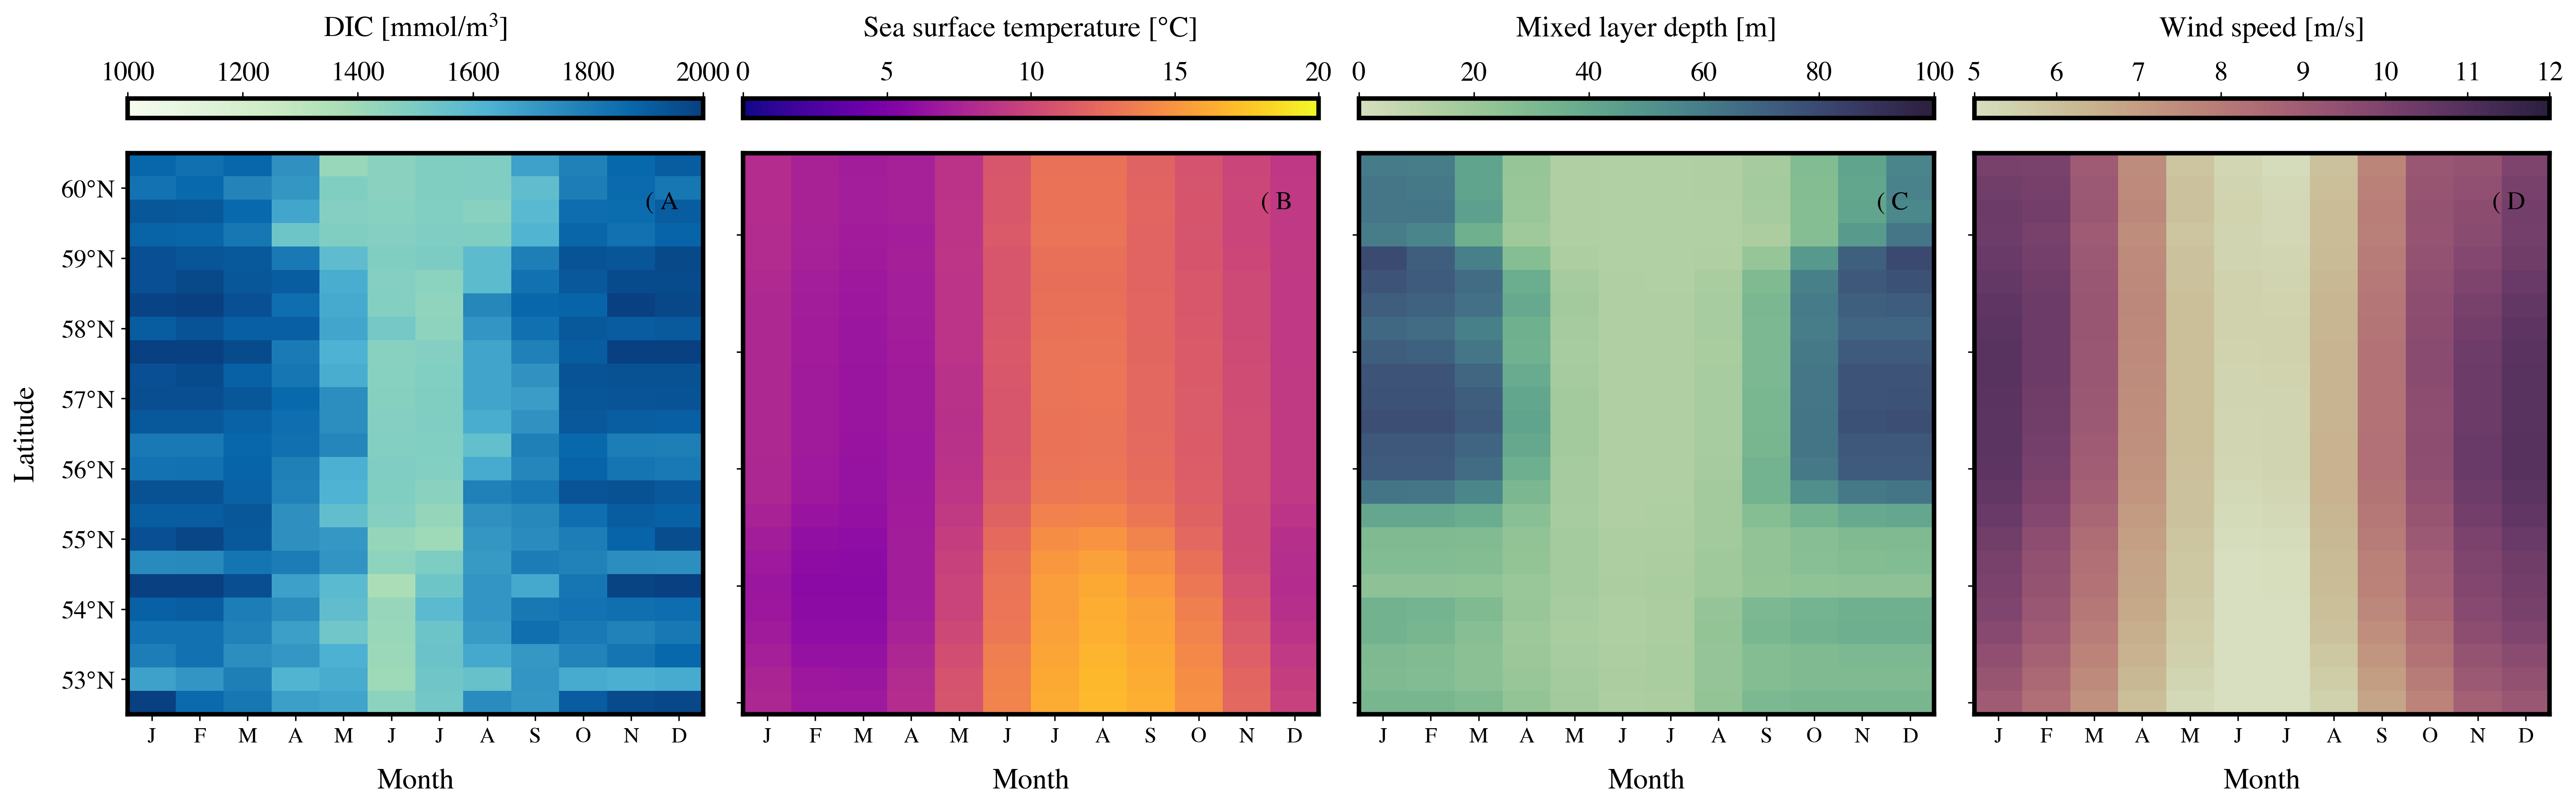
\includegraphics[width=15cm]{fig/1_Introduction/dsmw.png}

\end{figure}

On the other hand, in the southern North Sea and the adjacent European continental shelf, where high wind speed (D of \cref{dsmw}) and shallow water depth (C of \cref{dsmw}) generate a more uniform layer all year round \citep{thomas2009enhanced}, the air-sea \ch{CO2} exchange is mainly induced by temperature variability (B of \cref{dsmw}) \citep{salt2013variability}. Due to a shallow water column, carbon production and remineralisation happen within the same surface compartment, where \ch{CO2} can easily be transferred with the atmosphere \citep{prowe2009mechanisms, thomas2004enhanced}. Thus, community respiration outweighs \ac{pp}-driven photosynthesis \citep{artioli2012carbonate} and this area constitutes a weak \ch{CO2} source to the atmosphere \citep{prowe2009mechanisms}. 

\ch{pCO2} seasonality in the North Sea follows a well-established pattern induced by its two biogeochemical provinces defined above. The summer season is where this divide is most evident, as the spring bloom of \ac{pp} in the northern region poses the conditions for a strong \ch{CO2} undersaturation in the surface layer, whereas subsurface biological respiration enhances the \ac{dic} pool far from the atmosphere. Conversely, the southern North Sea quickly becomes oversaturated with respect to surface \ch{CO2} content owing to the slowdown of \ac{pp} and temperature rise \citep{thomas2004enhanced}. 

In marginal seas like the North Sea, alkalinity seasonality remains relatively homogeneous. Especially in the southern, shallower waters, the seasonal cycle of alkalinity is a combination of a multitude of physical and biological interactions. Among others, the most important sources of alkalinity are runoff and water-sediment relations \citep{omar2010spatiotemporal}, together with the anaerobic degradation of \ac{om}, especially in the Wadden Sea. In general terms, this results in highest alkalinity levels in summer and lowest in winter \citep{thomas2009enhanced}. 

Additionally, a 2013 study on the waterway contribution of alkalinity in the southern North Sea revealed that river loads of nutrients have a relatively small impact on the observed alkalinity due to low concentrations in the Elbe river. On the other hand, the Wadden Sea holds a remarkable 68\% contribution to annual alkalinity levels in the region \citep{schwichtenberg2013drivers}. 

pH is intrinsically connected to the processes described above. In the northern North Sea, more biologically active, \ch{CO2} export at the surface layer maintains a relatively high pH, while \ac{om} respiration in southern waters triggers pH decline \citep{salt2013variability, thomas2004enhanced}. Whereas this pH divide is hardly detectable in winter, a strong North-to-South gradient is registered in summer: southern water pH is reduced whereas northern pH is enhanced \citep{thomas2009enhanced}. 

\newpage\cleardoublepage
\chapter{Methods:}

\section{Model overview:}

In order to investigate the seasonal variations of \ch{CO2} and ocean \ch{pCO2} fluxes with enhanced alkalinity, output data from two model simulations were provided by GEOMAR Helmholtz Zentrum für Ozeanforschung (Kiel, Germany) in a netCDF format and analysed using Python programming language. This manuscript is therefore accompanied by a Data Management Plan that follows the outline provided by Wageningen University. Additionally, all scripts will be made freely available on the author's GitHub repository to allow for replication and encourage open-source research. 

The data used for this manuscript is derived from the \ac{foci} model, an emission-driven \ac{esm} that consists of an atmosphere, an ocean and a land surface component. The atmosphere is divided into 95 vertical layers and the ocean into 46 vertical layers, and the two components are coupled by the model every three hours. The ocean model has a spatial resolution of 1/2\textdegree{} on a tripolar grid. 

\ac{foci} incorporates the \ac{mops} to enable the simulation of marine biogeochemical cycles (\cref{foci-mops}) \citep{chien2022foci}. In its primitive version, \ac{mops} simulated the elemental cycle of phosphorous, nitrogen, and oxygen. When integrated into \ac{foci}, a full carbon cycle including \ac{dic} and alkalinity tracers was implemented. This allowed to resolve biological dynamics such as phytoplankton uptake and remineralisation, calcite formation and dissolution. \ac{foci}-\ac{mops} undergoes a 500-year spin-up, after which steady state is achieved for all variables, with the commonly-observed exception of nitrogen \citep{chien2022foci}.

\begin{figure}[H]
\caption[Schematic of the biogeochemistry in \texorpdfstring{FOCI}{FOCI}-\texorpdfstring{MOPS}{MOPS}.]{Schematic of the biogeochemistry in \ac{foci}-\ac{mops}. Arrows represent the interactions between different compartments.}
\label{foci-mops}
\centering
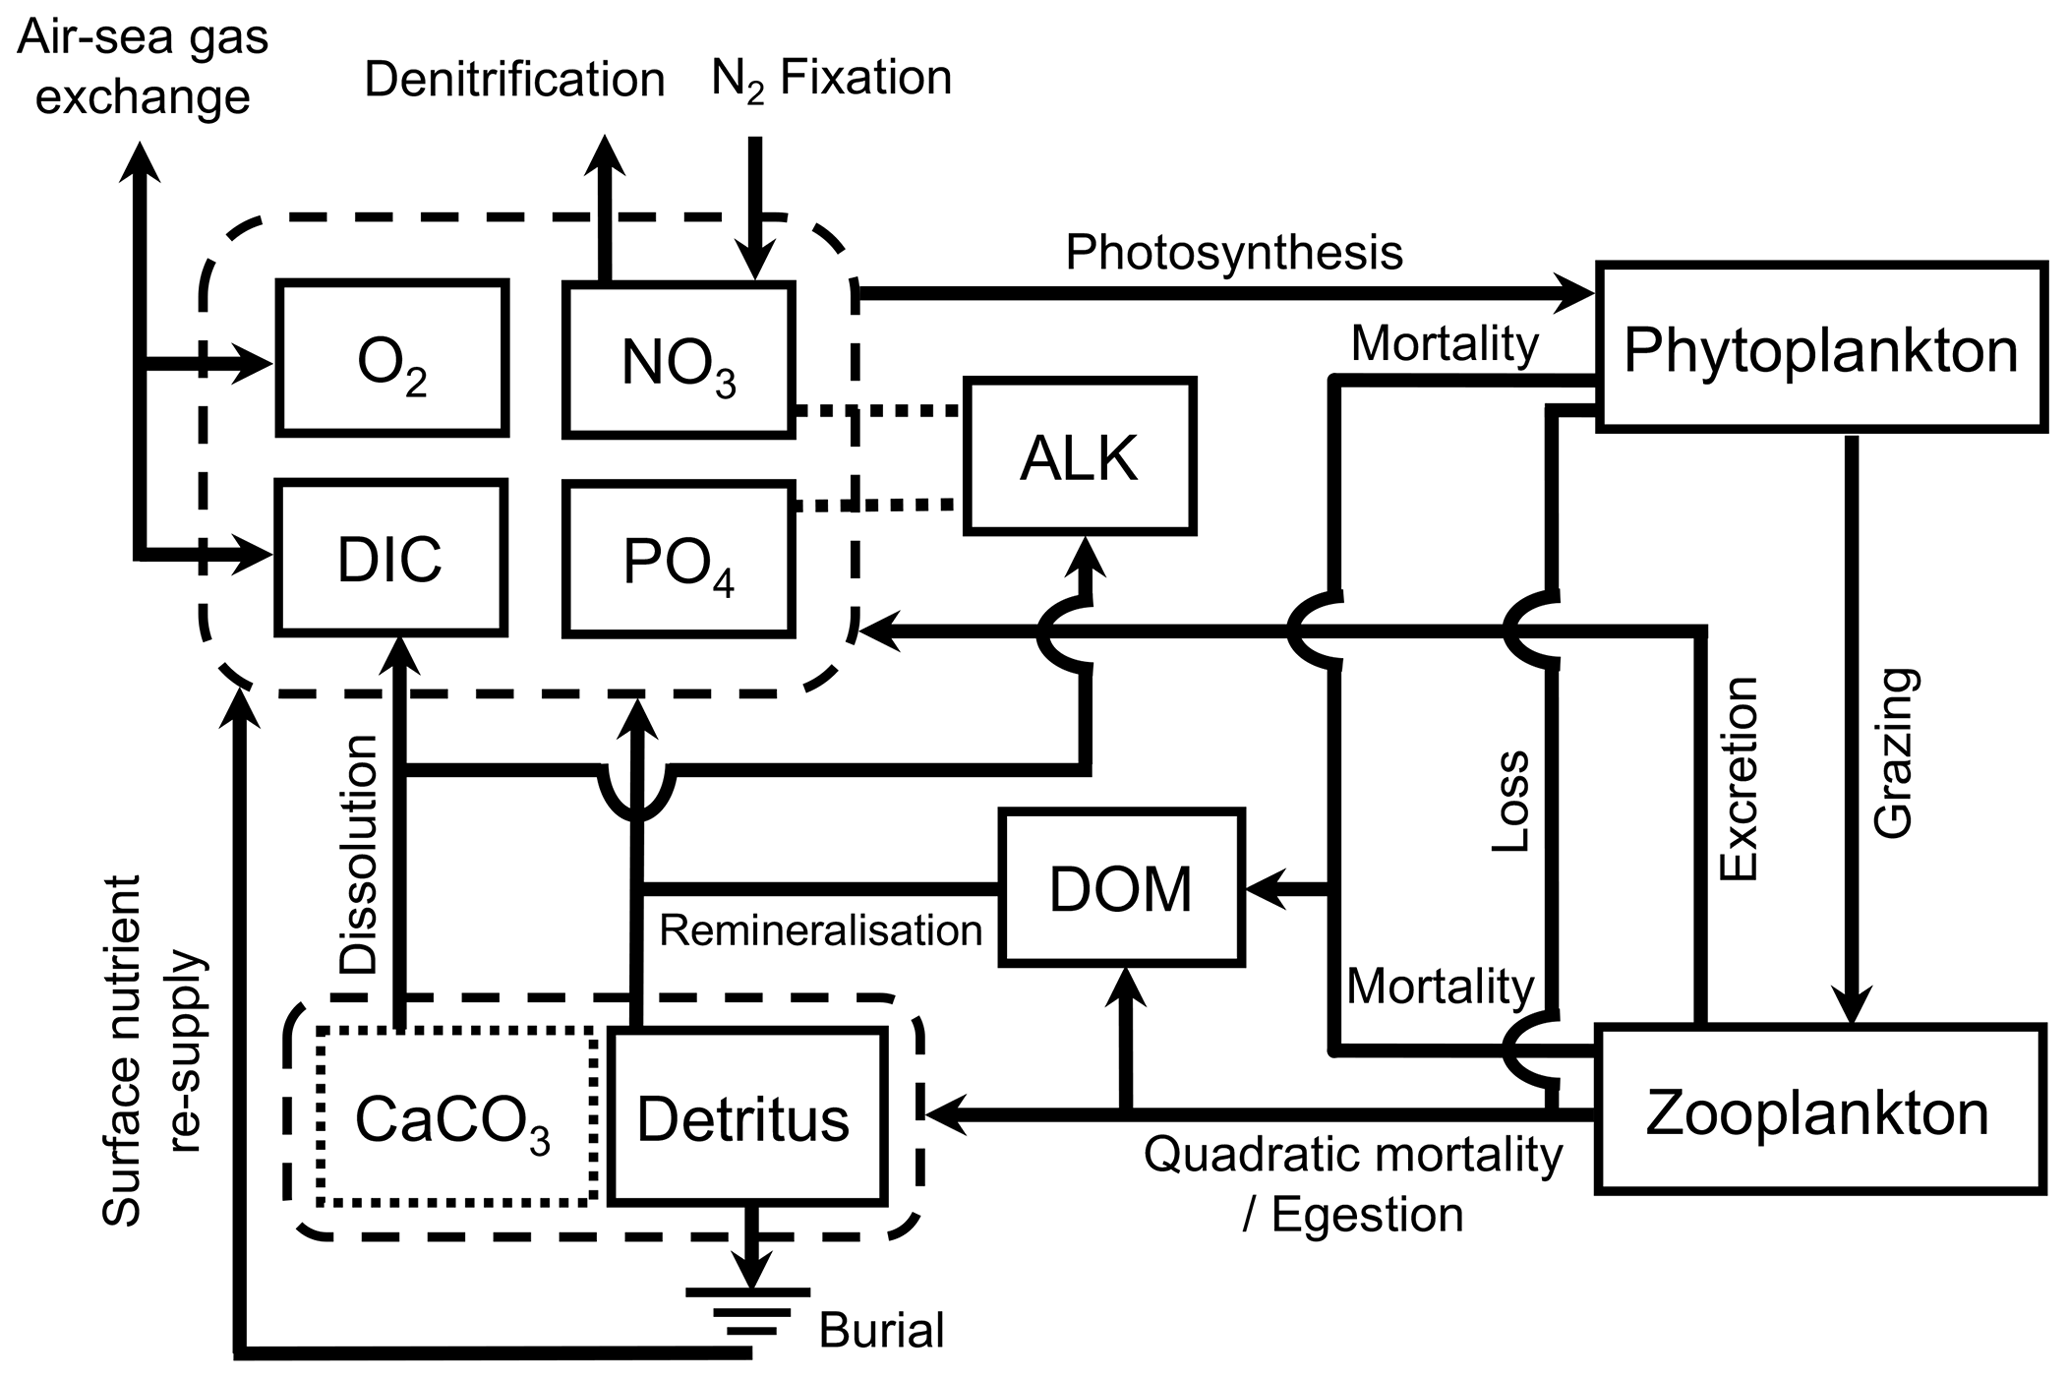
\includegraphics[width=12cm]{fig/1_Introduction/foci-mops.png}

\scriptsize Source: \cite{chien2022foci}
\end{figure}

Historical simulations were run from the year 1850 to the year 2015, from which the \ac{ssp} scenarios start. The simulations with alkalinity addition begin in year 2025 until 2100, with monthly time-steps. Alkalinity addition is simulated along the European coastline of 50-kilometre width, with the exclusion of the Baltic and the Mediterranean seas that are poorly resolved by the model. In \ac{foci}, alkalinity is a prognostic tracer simulated as a combination of biological sources and sinks: nitrate and phosphate supply as sinks, calcium carbonate production and dissolution as sink and source, respectively, and \ac{om} formation and remineralisation, as sink and source, respectively (\cref{foci-mops}) \citep{chen2021quantifying}. 

Two baseline \ac{ssp} scenarios were considered for the analysis. The first is SSP1-2.6 and describes a low-emission future with a radiative forcing of 2.6 W m\textsuperscript{-2} by the end of the century. This scenario prescribes strong emission abatement policies and reaches a limited warming below 2\textdegree C. The second is SSP3-7.0 and narrates a high-emission future with a radiative forcing of 7.0 W m\textsuperscript{-2} by 2100. This scenario lacks ambitious emission reduction strategies, implies relatively strong land use change and has a warming potential of about 4\textdegree C compared to pre-industrial levels \citep{o2016scenario}. 

\ac{oae} is simulated in \ac{foci} using a masking approach. Alkalinity is added to the system continuously and uniformly along the European coast (blue bordering line in \cref{oaemodel}) through the incorporation of fast-reacting quicklime on the ocean surface which is then allowed to diffuse over the domain. Alkalinity addition is subject to a linear increase over a 10-year period until the equivalent of 1 Gt yr\textsuperscript{-1} of calcium hydroxide (\ch{Ca(OH)2}) is reached. The latter consumes two moles of atmospheric \ch{CO2} and produces one mole of calcium (\ch{Ca}\textsuperscript{2+}) and two moles of bicarbonate ions (\ch{HCO3-}), therefore ideally increasing alkalinity by a factor of two (see \eqref{eqn:calc}) \citep{chien2022foci}. 

\begin{center}

\begin{equation} 
\label{eqn:calc}
\ch{Ca(OH)2} + 2\ch{CO2} \leftrightarrow \ch{Ca}\textsuperscript{2+} + 2\ch{HCO3-}
\end{equation}

\end{center}

\begin{figure}[H]
\caption[\texorpdfstring{OAE}{OAE} application in the study area]{Geographical \ac{oae} application in the study area}
\label{oaemodel}
\centering
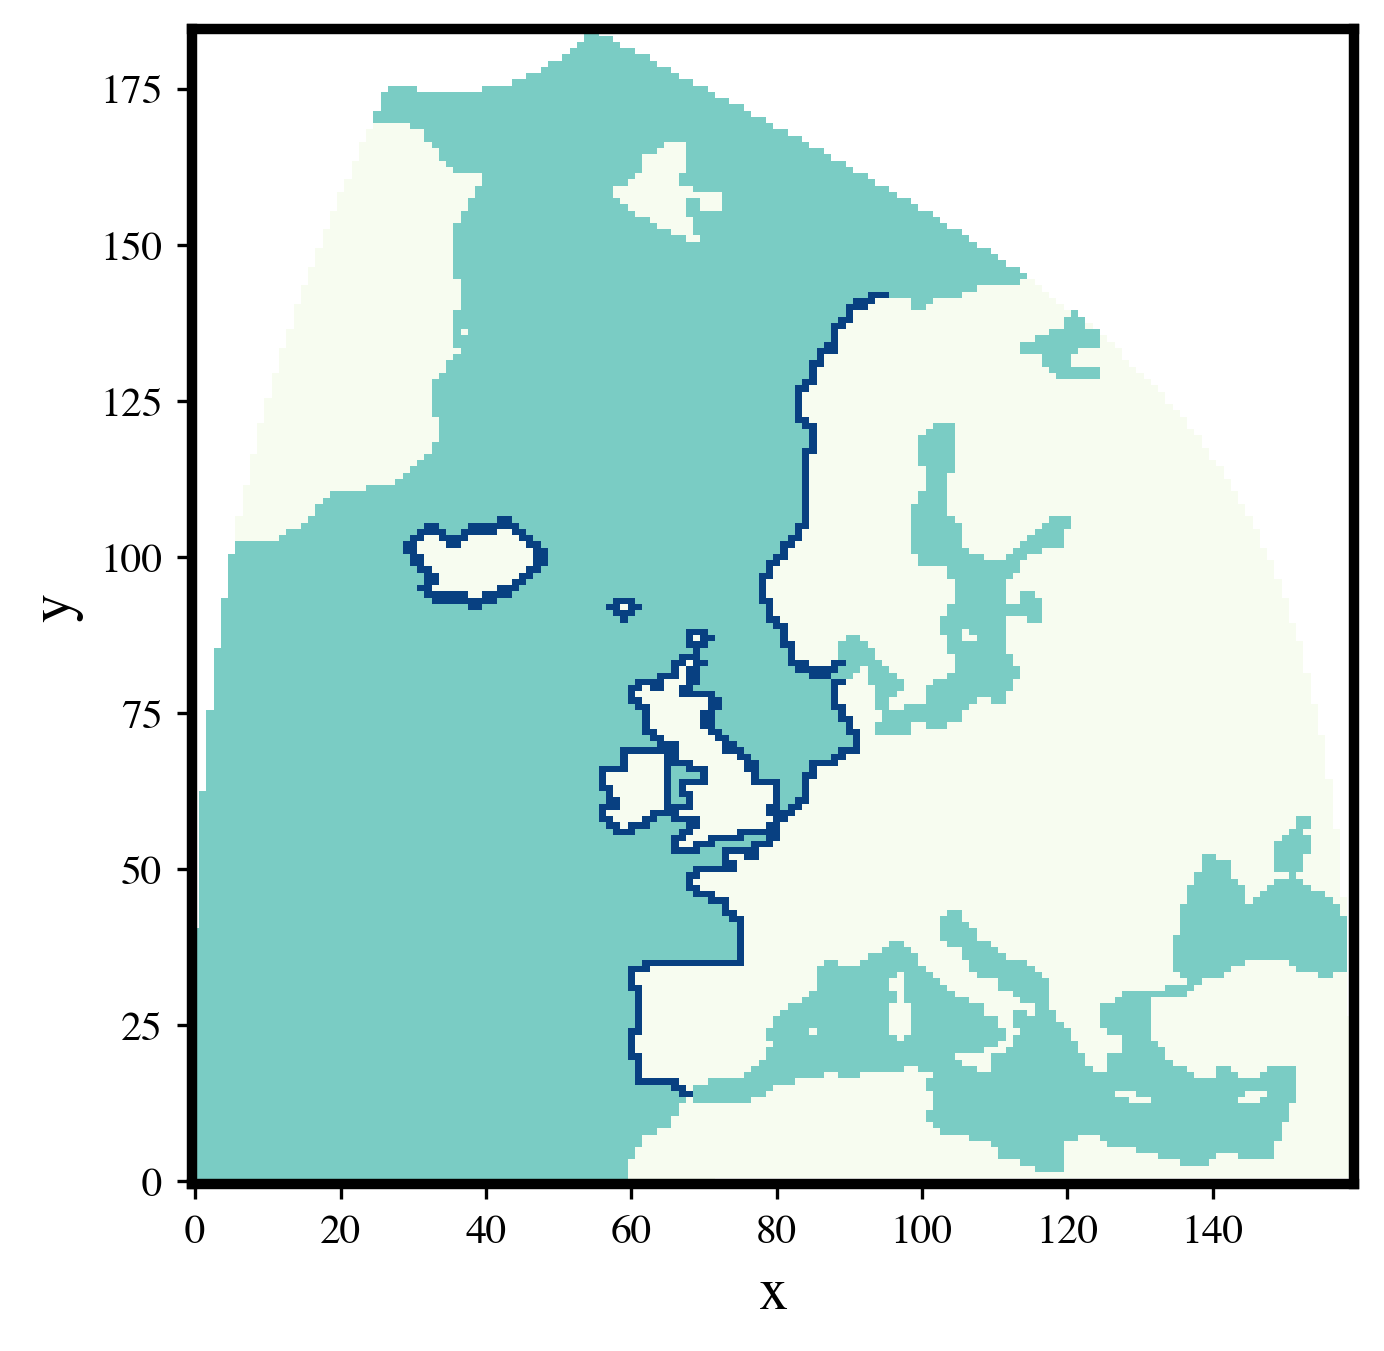
\includegraphics[width=10cm]{fig/2_Methods/mesh_mask_area.png}

\end{figure}

The parameterisation of air-sea gas exchange in \ac{foci} is described by the following equation:

\begin{center}

\begin{equation}
\label{eqn:1.1}
F_{ \ch{CO2} }  =  k_{w} ([ \ch{CO2*}]_{sat} -[ \ch{CO2*}]) 
\end{equation}

\end{center}

where $ k_{w} $ is the gas transfer velocity in m s\textsuperscript{-1}, $ \ch{CO2*}_({sat}) $ is the saturation concentration of \ch{CO2} in mol kg\textsuperscript{-1}, and $ \ch{CO2*} $ is the surface ocean dissolved \ch{CO2} concentration in mol kg\textsuperscript{-1} \citep{chien2022foci}.

Ocean \ch{pCO2}, that in \ac{foci} is termed surface \ch{CO2} fugacity $(f\ch{CO2})$, is calculated as follows:

\begin{center}

\begin{equation}
\label{eqnfCO2}
f{ \ch{CO2} } = \ch{CO2*} / K\textsubscript{0} 
\end{equation}
    
\end{center}

where K\textsubscript{0} is the solubility coefficient of \ch{CO2} in seawater. Both factors are affected by a multitude of intertwined physical and biological processes which are sometimes difficult to analyse individually. Some of the variables may also be subject to over and underestimation, therefore altering connected interactions \citep{chien2022foci}. 

\section{Descriptive analysis and data pre-processing:}

The methodology of this study consists of a descriptive analysis and splits in two parts. First, the focus is put on the European area and seasonality is calculated to account for regional averages. Then, the analysis zooms in a specific geographical point termed S, which was arbitrarily assigned off of the Dutch coasts, at 52\degree N and 3\degree E (red circle in figure \Cref{cropping}). This is done with the aim of visualising the differences and similarities between the system as a whole and the epicentre of the experiment domain in the southern North Sea. 

The global output data was sliced to the European coastline, with coordinates -25\degree{} to 10\degree{} E and 40\degree{} to 70\degree{} N. As found in \cref{cropping}, the cropped area does not cover the entire European region where \ac{oae} was performed, and part of the Norwegian and Spanish littoral were left out of the analysis. This approximation was due to time constraints and does not result in a meaningful modification from the actual regional definition. 

\begin{figure}[H]
\caption[Cropping of the study area and geographical location of point S]{Cropping of the study area (left) and geographical location of point S (right)}
\label{cropping}
\centering
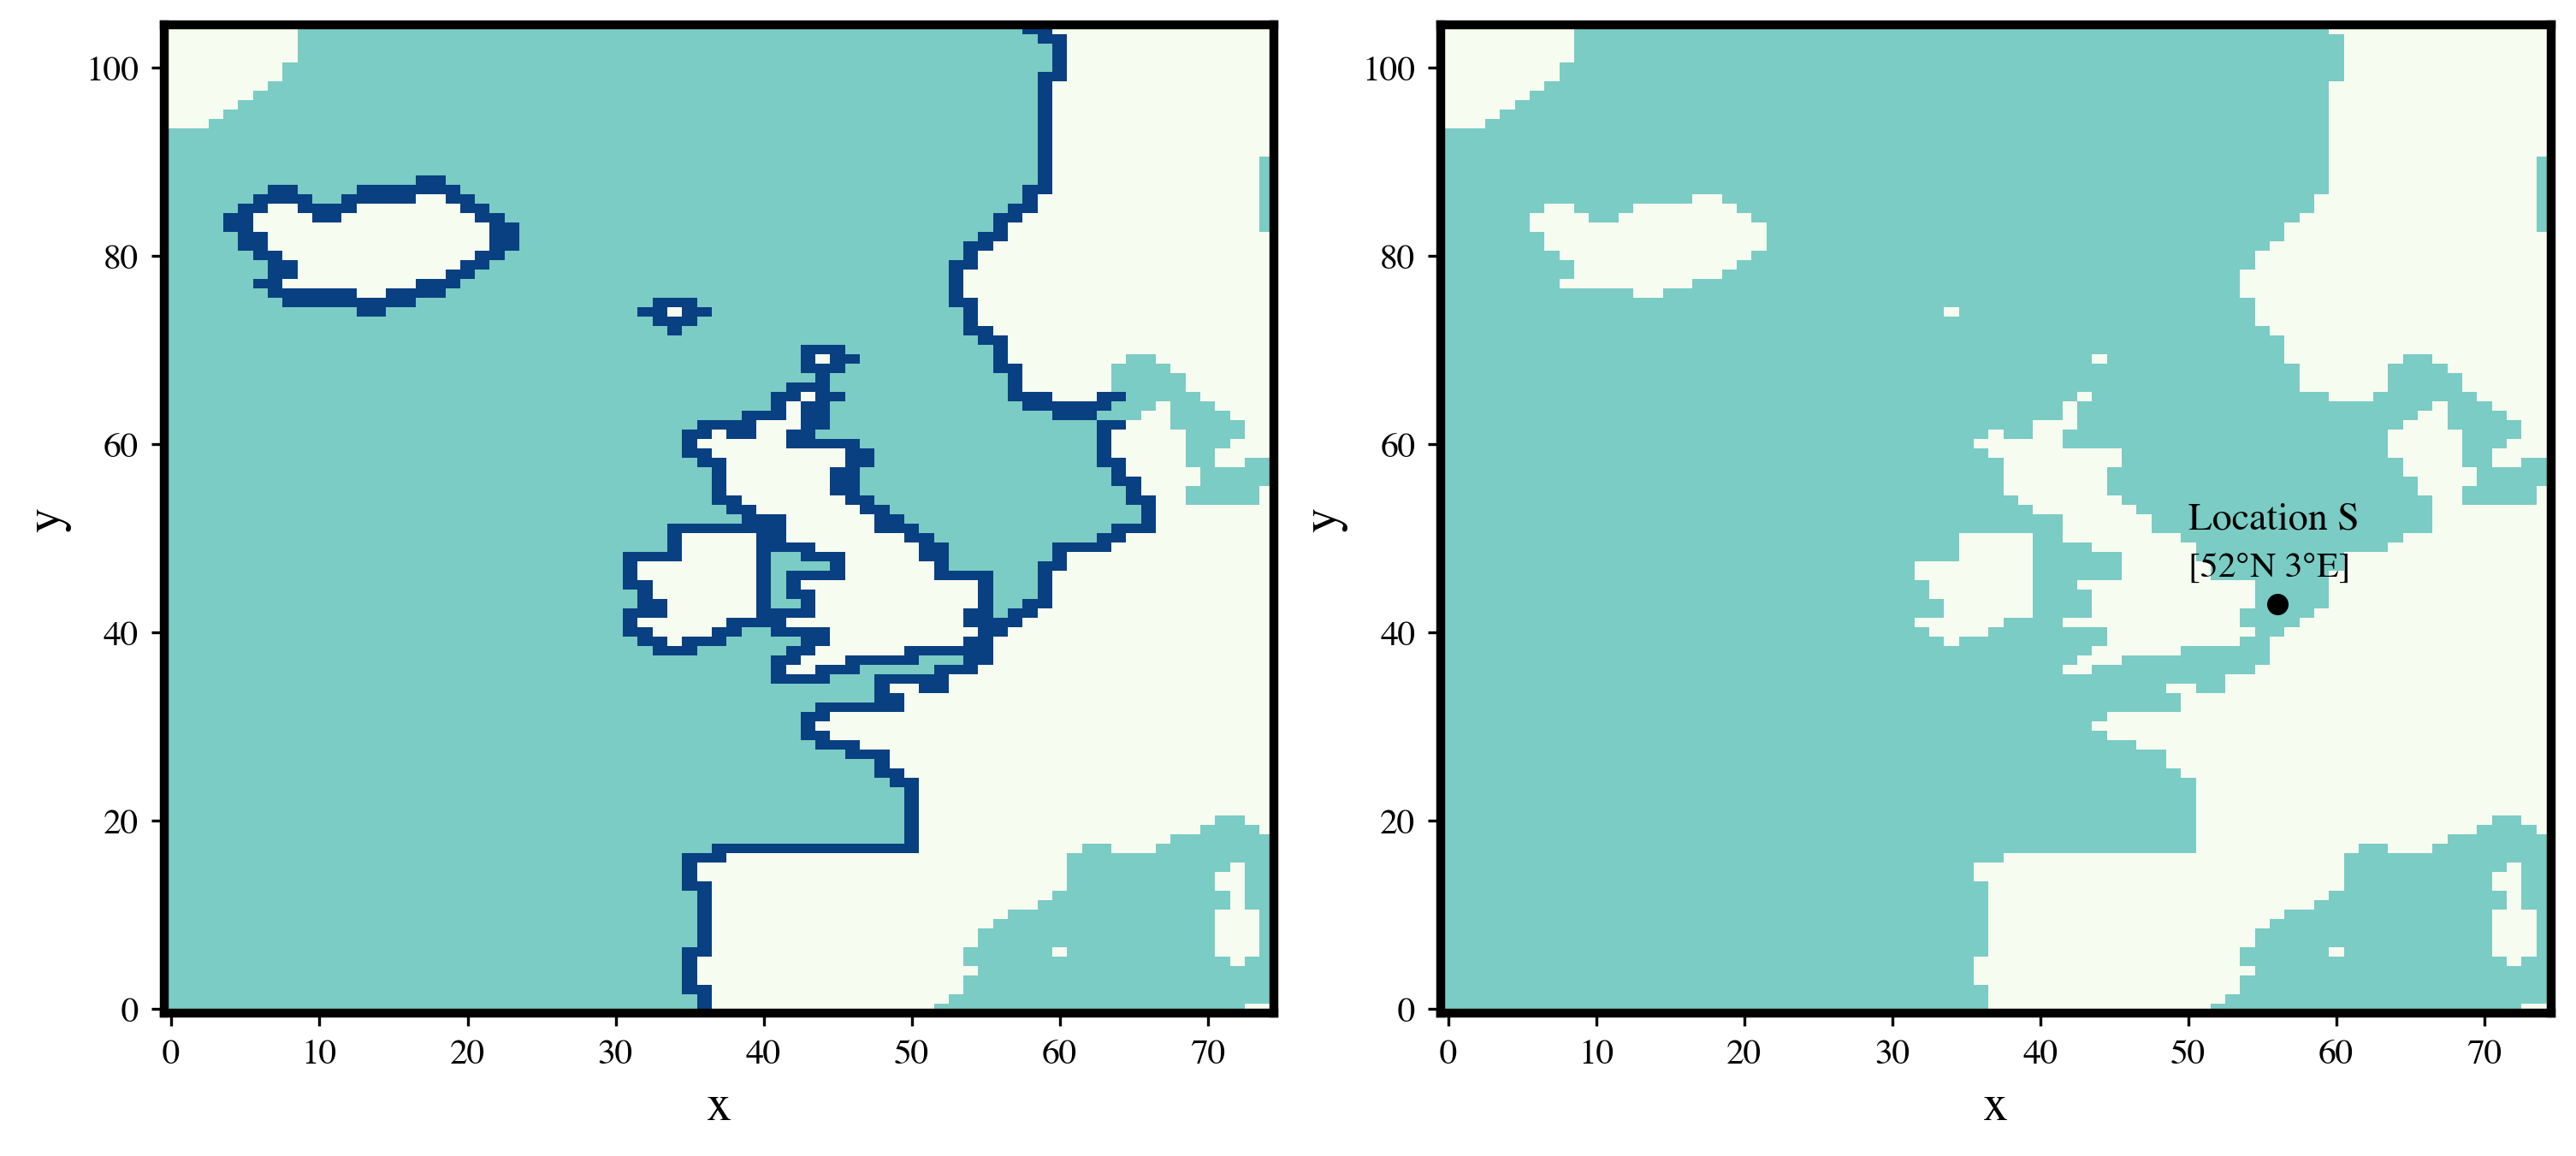
\includegraphics[width=15cm]{fig/2_Methods/mesh_mask_point.png}

\end{figure}

As previous studies suggest that seasonal trends detected at the ocean surface emerges after around ten years, a decadal trend investigation was conducted, drawing from \cite{wang2023simulated}. Additionally, seasonal discrepancies between the two scenarios were expected to be the most visible close to the simulation's end, when the system has stabilised. Therefore, the last 10 years registered by \ac{foci} (2090-2100) were selected. Due to a limited space, an annual average for the last decade is shown in this manuscript. 

Five main parameters were extracted from the simulation dataset, here presented in the order from drivers to outcome variables: alkalinity, pH, \ac{dic}, \ch{pCO2}, and \ch{CO2} flux. While \ch{CO2} flux, \ch{pCO2} and pH are designed 3-dimensionally, with a latitude, longitude and time dimension, \ac{dic} and alkalinity are also calculated over the 46 layers in which the ocean component of the model is divided. Therefore, the investigation of those variables takes the average over the ocean surface that was arbitrarily set at 50 metres. 

It is worth noting that, due to its shallow profile, in the southern North Sea, the depth of the water column is lower than 50 metres. At location S, for example, the maximum water depth goes as low as 16.3 m, which represents the third \ac{foci} layer. Additionally, in the model, each layer length increases as a function of depth, meaning a weighted average was performed over the selected range of 50 metres for alkalinity and \ac{dic}. 

A land mask was applied to discount all land values, which in the simulations correspond to 0 (with the exception of pH) and would therefore have altered the calculated absolute values. All variables were then re-averaged based on the grid cell area (for \ch{CO2} flux, \ch{pCO2} and pH) and volume (for \ac{dic} and alkalinity). Unlike the other four, \ch{CO2} flux calculations are performed in the atmospheric component of \ac{foci}, which has a grid resolution of $\sim$1.8\textdegree{}. This explains the coarser pattern in the \ch{CO2} flux plots presented below \citep{matthes2020flexible}.

To account for the volume of each grid cell, the units of \ac{dic} and alkalinity were transformed from µmol kg\textsuperscript{-1} to mmol m\textsuperscript{-3}. The datasets were divided by 1000 to convert µmol into mmol, and then multiplied by 1025 kg m\textsuperscript{-3}, that is, global potential seawater density. As for \ch{CO2} flux, the \ac{foci} output delivers the variable in kg m\textsuperscript{-2} s\textsuperscript{-1}. Although such unit is dominating in climate mitigation literature, it is noted that, in ocean-focused papers, air-sea \ch{CO2} flux is usually measured in mol m\textsuperscript{-2} yr\textsuperscript{-1}. Therefore, the datasets were converted into such unit multiplying by the number of seconds in one year (31,536,000 seconds) and dividing by the molar mass of carbon dioxide in mol kg\textsuperscript{-1}, that is, 0.04401 mol kg\textsuperscript{-1}.

To account for seasonality, the monthly mean data were arranged in groups of three and averaged to the corresponding seasonal value. The four seasons were delineated as follows: winter, which includes December, January and February (DJF); spring, gathering March, April and May (MAM); summer includes June, July and August (JJA); finally, September, October and November compose autumn (SON). Seasonal trends were calculated with a weighting method, which accounted for the number of days contained in each month composing the target season. Then, the seasons were ungrouped to investigate monthly means and sub-seasonal variations, therefore gaining higher accuracy. Lastly, drawing from \cite{jo2022future}, seasonal amplitude regional maps were drawn, where the seasonal amplitude is the difference between the annual maximum and the annual minimum for the defined variable. 

Different descriptive tools were utilised to visualise the data. Scatterplots and lineplots define European and location S averages: in the former, local differences are approximated and give an overview of how the European system as a whole will behave in the future; in the latter, taking the average over location S allows to draw conclusions of regime shifts close to the epicentre of the domain. Additionally, maps were used to identify local patterns and distinguish the alkalised and non-alkalised ocean behaviour in different geographical areas accounting, for example, for the vicinity to the injection sites or the access to open-ocean regions.

\section{Overview of the explored variables:}

This section provides a short summary of the variables explored in this manuscript and their representation in the \ac{foci} model in the order from drivers to affected outcomes.

\begin{itemize}
    \item Alkalinity: it is the property that defines seawater capacity to neutralise pH changes. In \ac{foci}, alkalinity is measured in µmol kg\textsuperscript{-1}, which was converted in mmol m\textsuperscript{-3}. Alkalinity is analysed over depth, calculating the average of the surface water set at 50 metres for the European average, and at 16.3 metres for location S (corresponding to the third \ac{foci} depth layer).
    \item \ac{dic}: the \ac{dic} pool incorporates the three carbon species that the ocean stores, namely \ch{HCO3-}, \ch{CO3^{2-}} and \ch{CO2}(aq). In \ac{foci}, \ac{dic} is measured in µmol kg\textsuperscript{-1}, then transformed to mmol m\textsuperscript{-3}, and its analysis is performed over depth, taking an average of the arbitrarily-set 50-metre depth.
    \item pH: it describes the changes in the seawater \ch{H+} concentration and, in \ac{foci}, it is registered only at the first ocean layer. 
    \item \ch{pCO2}: at the air-sea interface, it determines the direction of the gas flux: where atmospheric \ch{CO2} concentration is larger than the ocean's, \ch{CO2} is directed downwards, and viceversa. In \ac{foci}, \ch{pCO2} is measured in µatm (microatmospheres).
    \item \ch{CO2} flux: it represents the flux of carbon dioxide in and out of the ocean. In \ac{foci}, negative values correspond to ocean uptake and positive values to ocean outgassing. The variable is delivered by \ac{foci} in kg m\textsuperscript{-2} s\textsuperscript{-1}, which was converted to mol m\textsuperscript{-2} yr\textsuperscript{-1}.
\end{itemize}














\newpage\cleardoublepage
\chapter{Results:}

Tables \ref{amplSum26} and \ref{amplSum70} summarise the seasonal amplitude of all defined variables averaged over the last simulation decade, without and with alkalinity enhancement, for the European coastline and for location S under both emission scenarios. Below, each variable is then investigated in depth. 

\begin{center}

\begin{table}[H]
\captionof{table}[Seasonal amplitude average for alkalinity, pH, \texorpdfstring{DIC}{DIC}, \ch{pCO2}, and \ch{CO2} flux in SSP1-2.6.]{For SSP1-2.6, seasonal amplitude for alkalinity, pH, \ac{dic}, \ch{pCO2}, and \ch{CO2} flux averaged over 2090 to 2100.
\label{amplSum26}}

\scalebox{0.95}{
        \begin{tabular}{|| c || c c || c c || c ||} % c|l|r
    {} & \multicolumn{2}{c}{European average} 
    & 
    \multicolumn{2}{c}{Location S} \\
    {} & {Without \ac{oae}} & {With \ac{oae}} & {Without \ac{oae}} & {With \ac{oae}} & {Unit} \\
    \hline \hline
    {} & {} & {} & {} & {} \\
    Alkalinity & 11 & 5 & 25 & 215 & mmol m\textsuperscript{-3} \\
    pH & 0.027 & 0.017 & 0.139 & 0.143 & - \\
    \ac{dic} & 30 & 23 & 46 & 54 & mmol m\textsuperscript{-3} \\
    \ch{pCO2} & 35 & 23 & 166 & 51 & µatm \\
    \ch{CO2} flux & 2.69 & 3.88 & 8.17 & 16.49 & mol m\textsuperscript{-2} yr\textsuperscript{-1} \\
    \end{tabular}}
\end{table}

\end{center}

\begin{center}

\begin{table}[H]
\captionof{table}[Seasonal amplitude average for alkalinity, pH, \texorpdfstring{DIC}{DIC}, \ch{pCO2}, and \ch{CO2} flux in SSP3-7.0.]{For SSP3-7.0, seasonal amplitude for alkalinity, pH, \ac{dic}, \ch{pCO2}, and \ch{CO2} flux averaged over 2090 to 2100.\label{amplSum70}}

\scalebox{0.95}{
        \begin{tabular}{|| c || c c || c c || c ||} % c|l|r
    {} & \multicolumn{2}{c}{European average} 
    & 
    \multicolumn{2}{c}{Location S} \\
    {} & {Without \ac{oae}} & {With \ac{oae}} & {Without \ac{oae}} & {With \ac{oae}} & {Unit} \\
    \hline \hline
    {} & {} & {} & {} & {} \\
    Alkalinity & 13 & 6 & 44 & 354 & mmol m\textsuperscript{-3} \\
    pH & 0.029 & 0.018 & 0.099 & 0.159 & - \\
    \ac{dic} & 27 & 17 & 74 & 136 & mmol m\textsuperscript{-3} \\
    \ch{pCO2} & 73 & 55 & 207 & 112 & µatm \\
    \ch{CO2} flux & 4.34 & 6.38 & 9.24 & 28.26 & mol m\textsuperscript{-2} yr\textsuperscript{-1} \\
        \end{tabular}}
\end{table}

\end{center}

\section{Alkalinity:}

\begin{figure}[H]
\caption[Monthly average of baseline and \texorpdfstring{OAE}{OAE}-induced alkalinity]{From left to right, monthly average of baseline and \ac{oae}-induced alkalinity (mmol m\textsuperscript{-3}) in the European region in SSP1-2.6 (A), and in SSP3-7.0 (C), and at location S in SSP1-2.6 (E) and in SSP3-7.0 (G) averaged over 2090-2100 (top), and the difference ($\Delta$) (B, D, F, and H) between the two scenarios (bottom).}
\label{alkalinity}
\centering
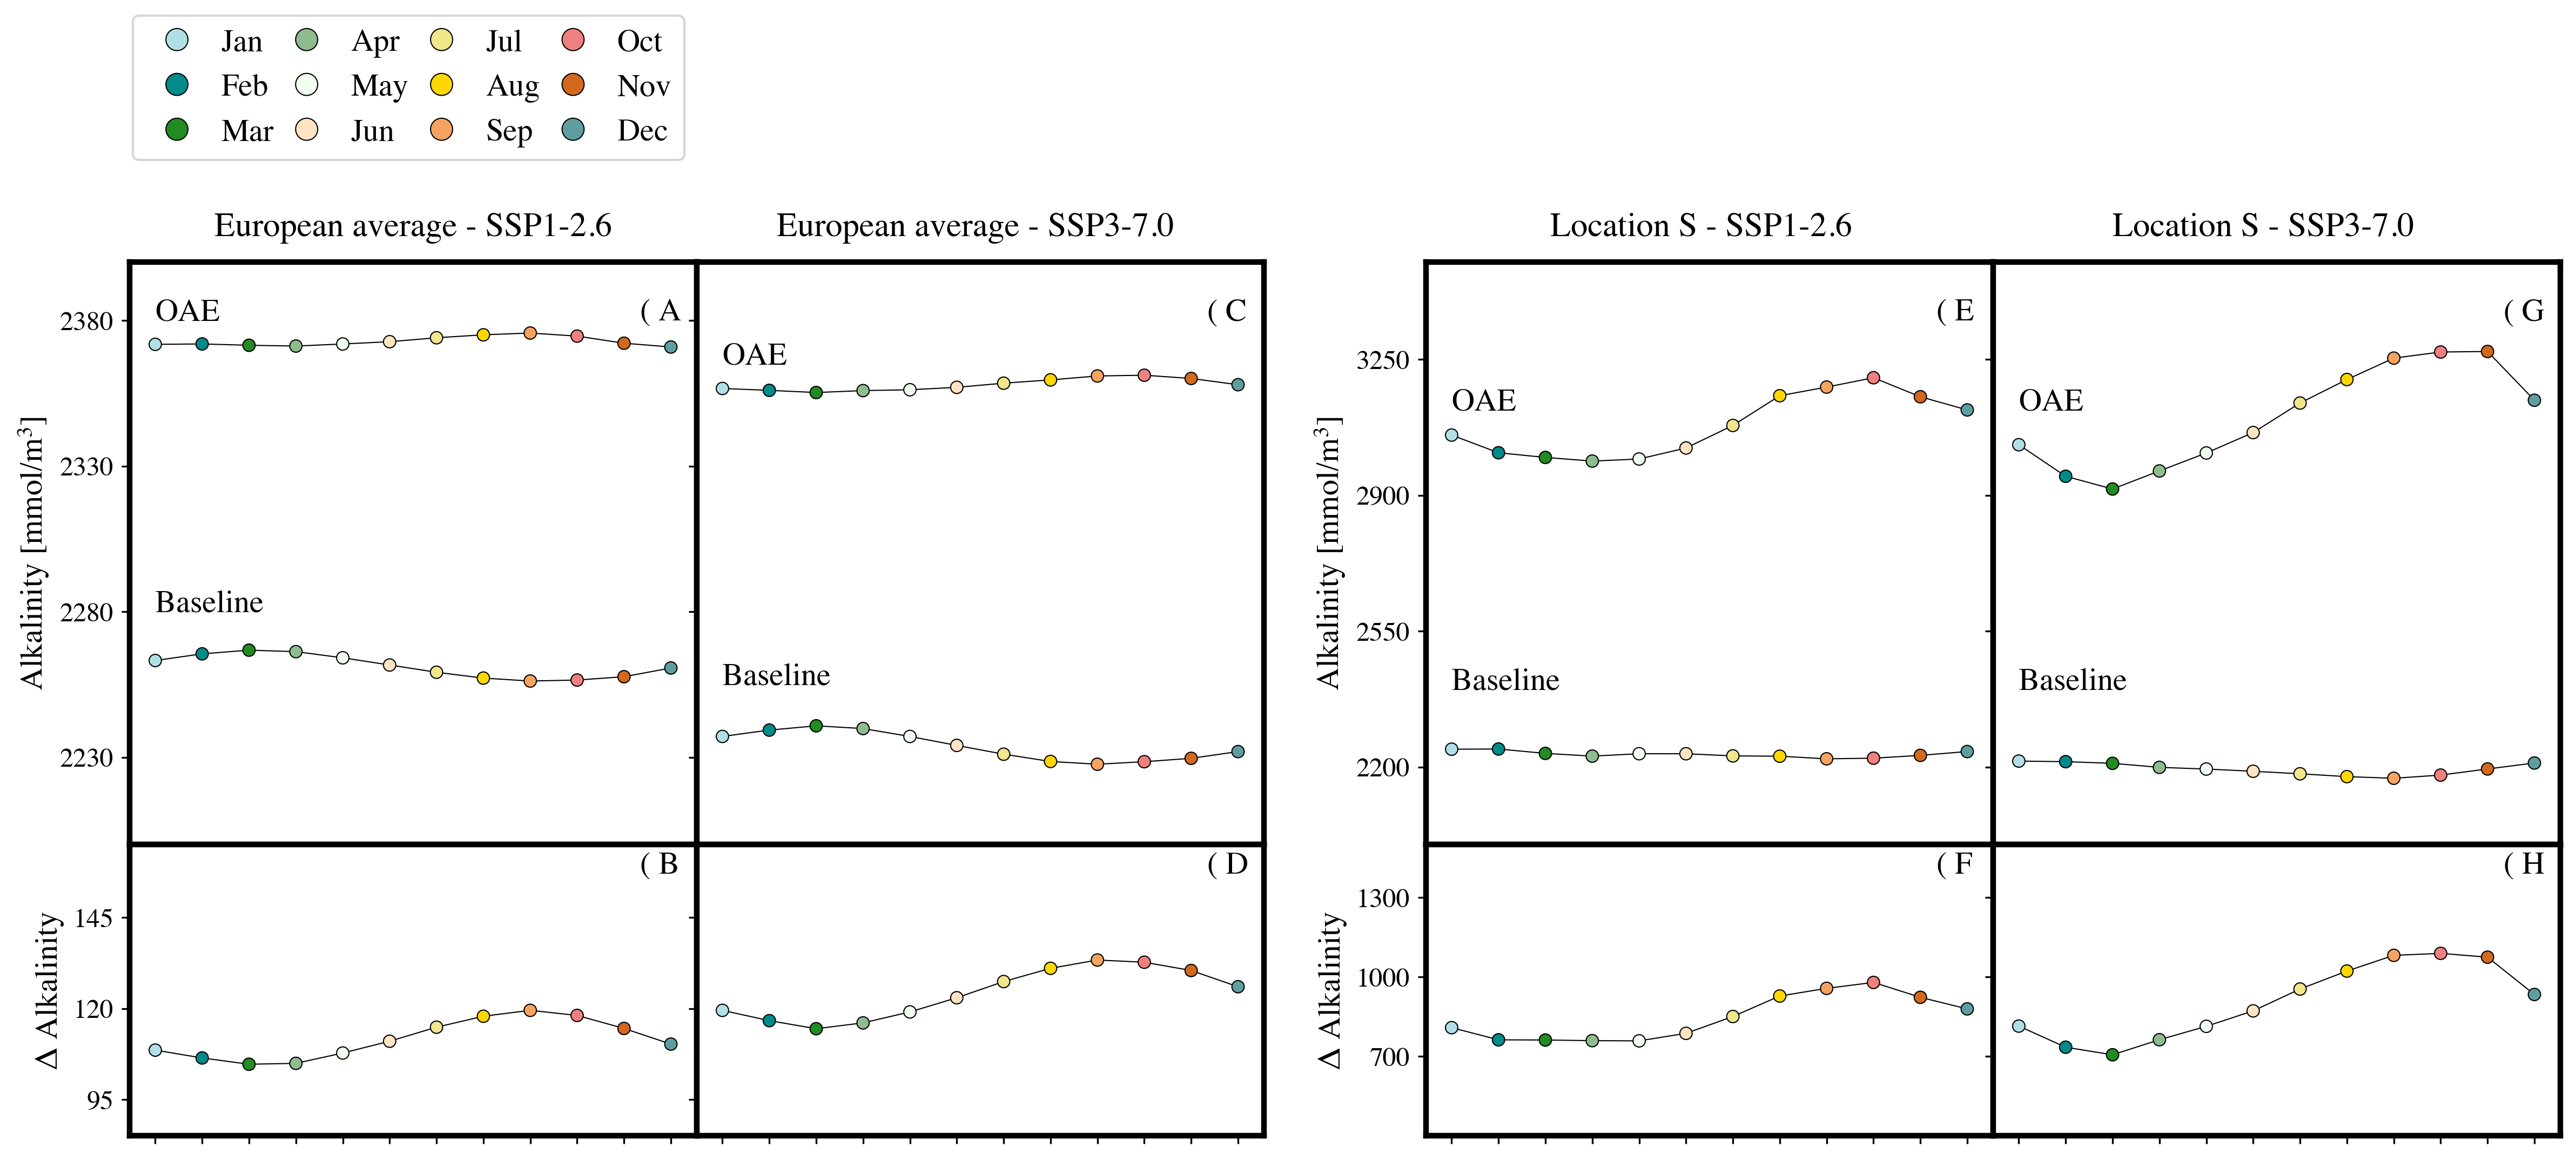
\includegraphics[width=15cm]{fig/3_Results/Alkalinity/alkalinity.png}

\end{figure}

The baseline alkalinity seasonality in SSP1-2.6 in the European region stretches between highest values at the onset of spring and lowest values in autumn. Maxima and minima are recorded in March and October, respectively. The average amplitude spans between 2256 and 2267 mmol m\textsuperscript{-3}. In the \ac{oae} scenario, absolute values of alkalinity ramp up due to alkalinity addition. A of \cref{alkalinity} portrays a flattening of the line and seasonality is halved, with a current mean amplitude of 5 mmol m\textsuperscript{-3}. Lowest and highest alkalinity are now recorded in April and September, respectively (C of \cref{alkalinity}), revealing a strong alteration of the baseline seasonal cycle. The baseline high-emission scenario displays absolute values that are slightly lower than SSP1-2.6, with a mean seasonal range between 2228 and 2241 mmol m\textsuperscript{-3} in summer and winter, respectively. Similar to SSP1-2.6, alkalinity enhancement forces the annual cycle to a shift, where maxima are displayed in November and minima in March, with a decreased amplitude of 6 mmol m\textsuperscript{-3}. 

At location S in SSP1-2.6, \ac{oae} induces alkalinity absolute values to rise greatly and, unlike the European mean, the annual amplitude is enhanced (E of \cref{alkalinity}). The annual cycle shifts to high peaks in October and bottom peaks in April with an average range between 2988 and 3203 mmol m\textsuperscript{-3}, therefore exceeding by far the baseline amplitude of only 25 mmol m\textsuperscript{-3}. Higher atmospheric \ch{CO2} concentrations magnify the observed seasonal amplification (G of \cref{alkalinity}). Additionally, all $\Delta$ (B, D, F, and H of \cref{alkalinity}) reveal the highest baseline-to-\ac{oae} variation between September and October.

\begin{figure}[H]
\caption[European monthly average of baseline and \texorpdfstring{OAE}{OAE}-induced alkalinity as a function of depth]{European monthly average of baseline and \ac{oae}-induced alkalinity (mmol m\textsuperscript{-3}) as a function of depth (m) averaged over 2090-2100 (left). Grey lines define the \ac{foci} ocean layers. European monthly average of alkalinity (mmol m\textsuperscript{-3}) at the first \ac{foci} layer over 2090-2100 (right).}
\label{EUalkalinitysurface}
\centering
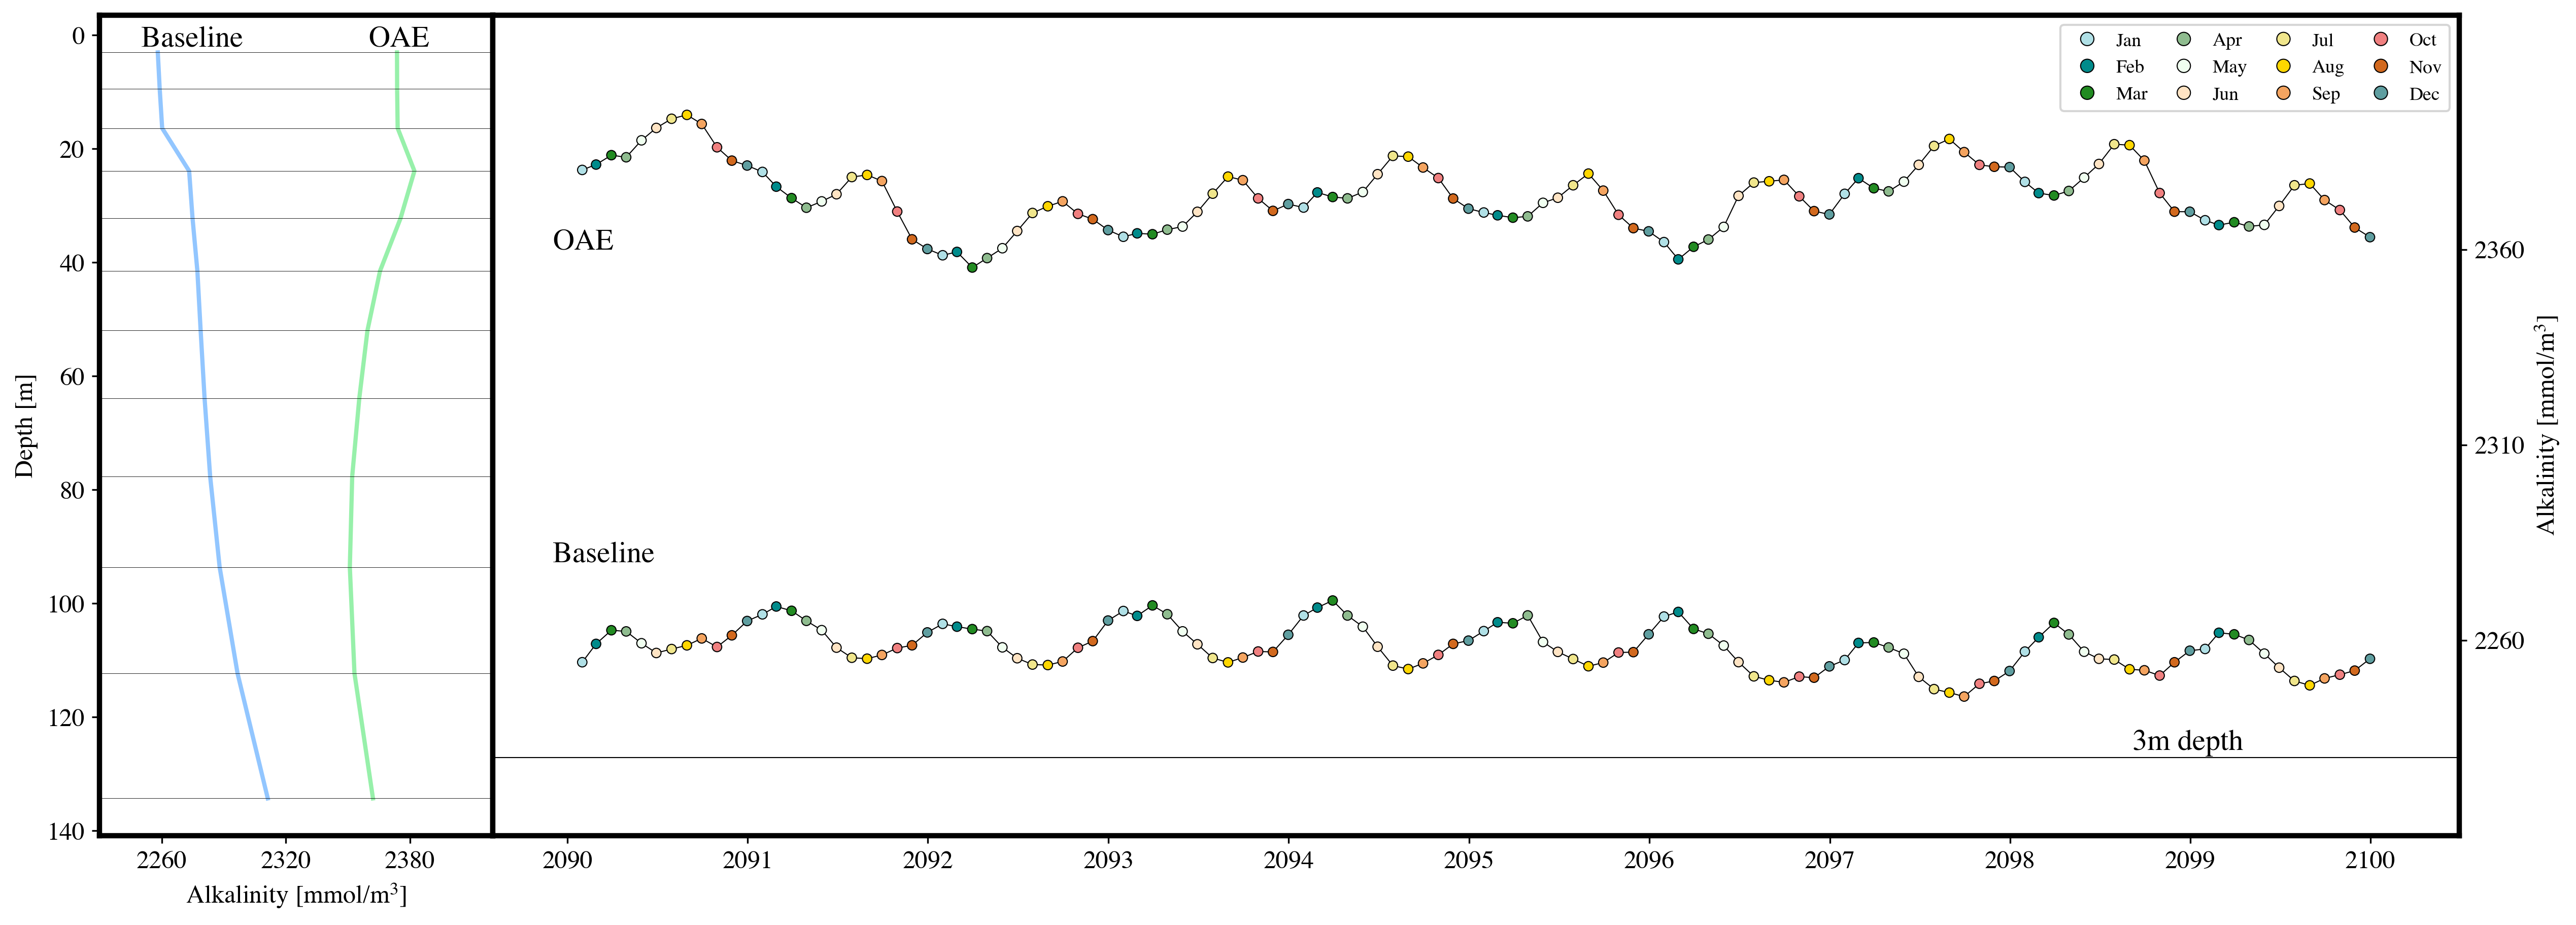
\includegraphics[width=15cm]{fig/3_Results/Alkalinity/EUAlk_depthprof.png}

\end{figure}

To explain the seasonal cycle alteration visible in A and C of \cref{alkalinity}, \cref{EUalkalinitysurface} shows the decadal mean of alkalinity for the first 3 metres of the ocean surface, where an evident reversal is recorded (right). On the left graph, alkalinity is plotted as a function of depth: the baseline values increase when moving deeper whereas the \ac{oae} has highest alkalinity at the surface (where it is added in the experiments) and progressively decreases up to about 90 metres, when it starts rising again. The reason for such a diversion is connected with the alteration of the alkalinity natural distribution through water column. 

\begin{figure}[H]
\caption[Alkalinity seasonal amplitude change]{Alkalinity seasonal amplitude change (mmol m\textsuperscript{-3}) without \ac{oae} (left), with \ac{oae} (middle), and the difference ($\Delta$) between the two (right). SSP1-2.6 (top) and SSP3-7.0 (bottom).}
\label{alkalinityamplitude}
\centering
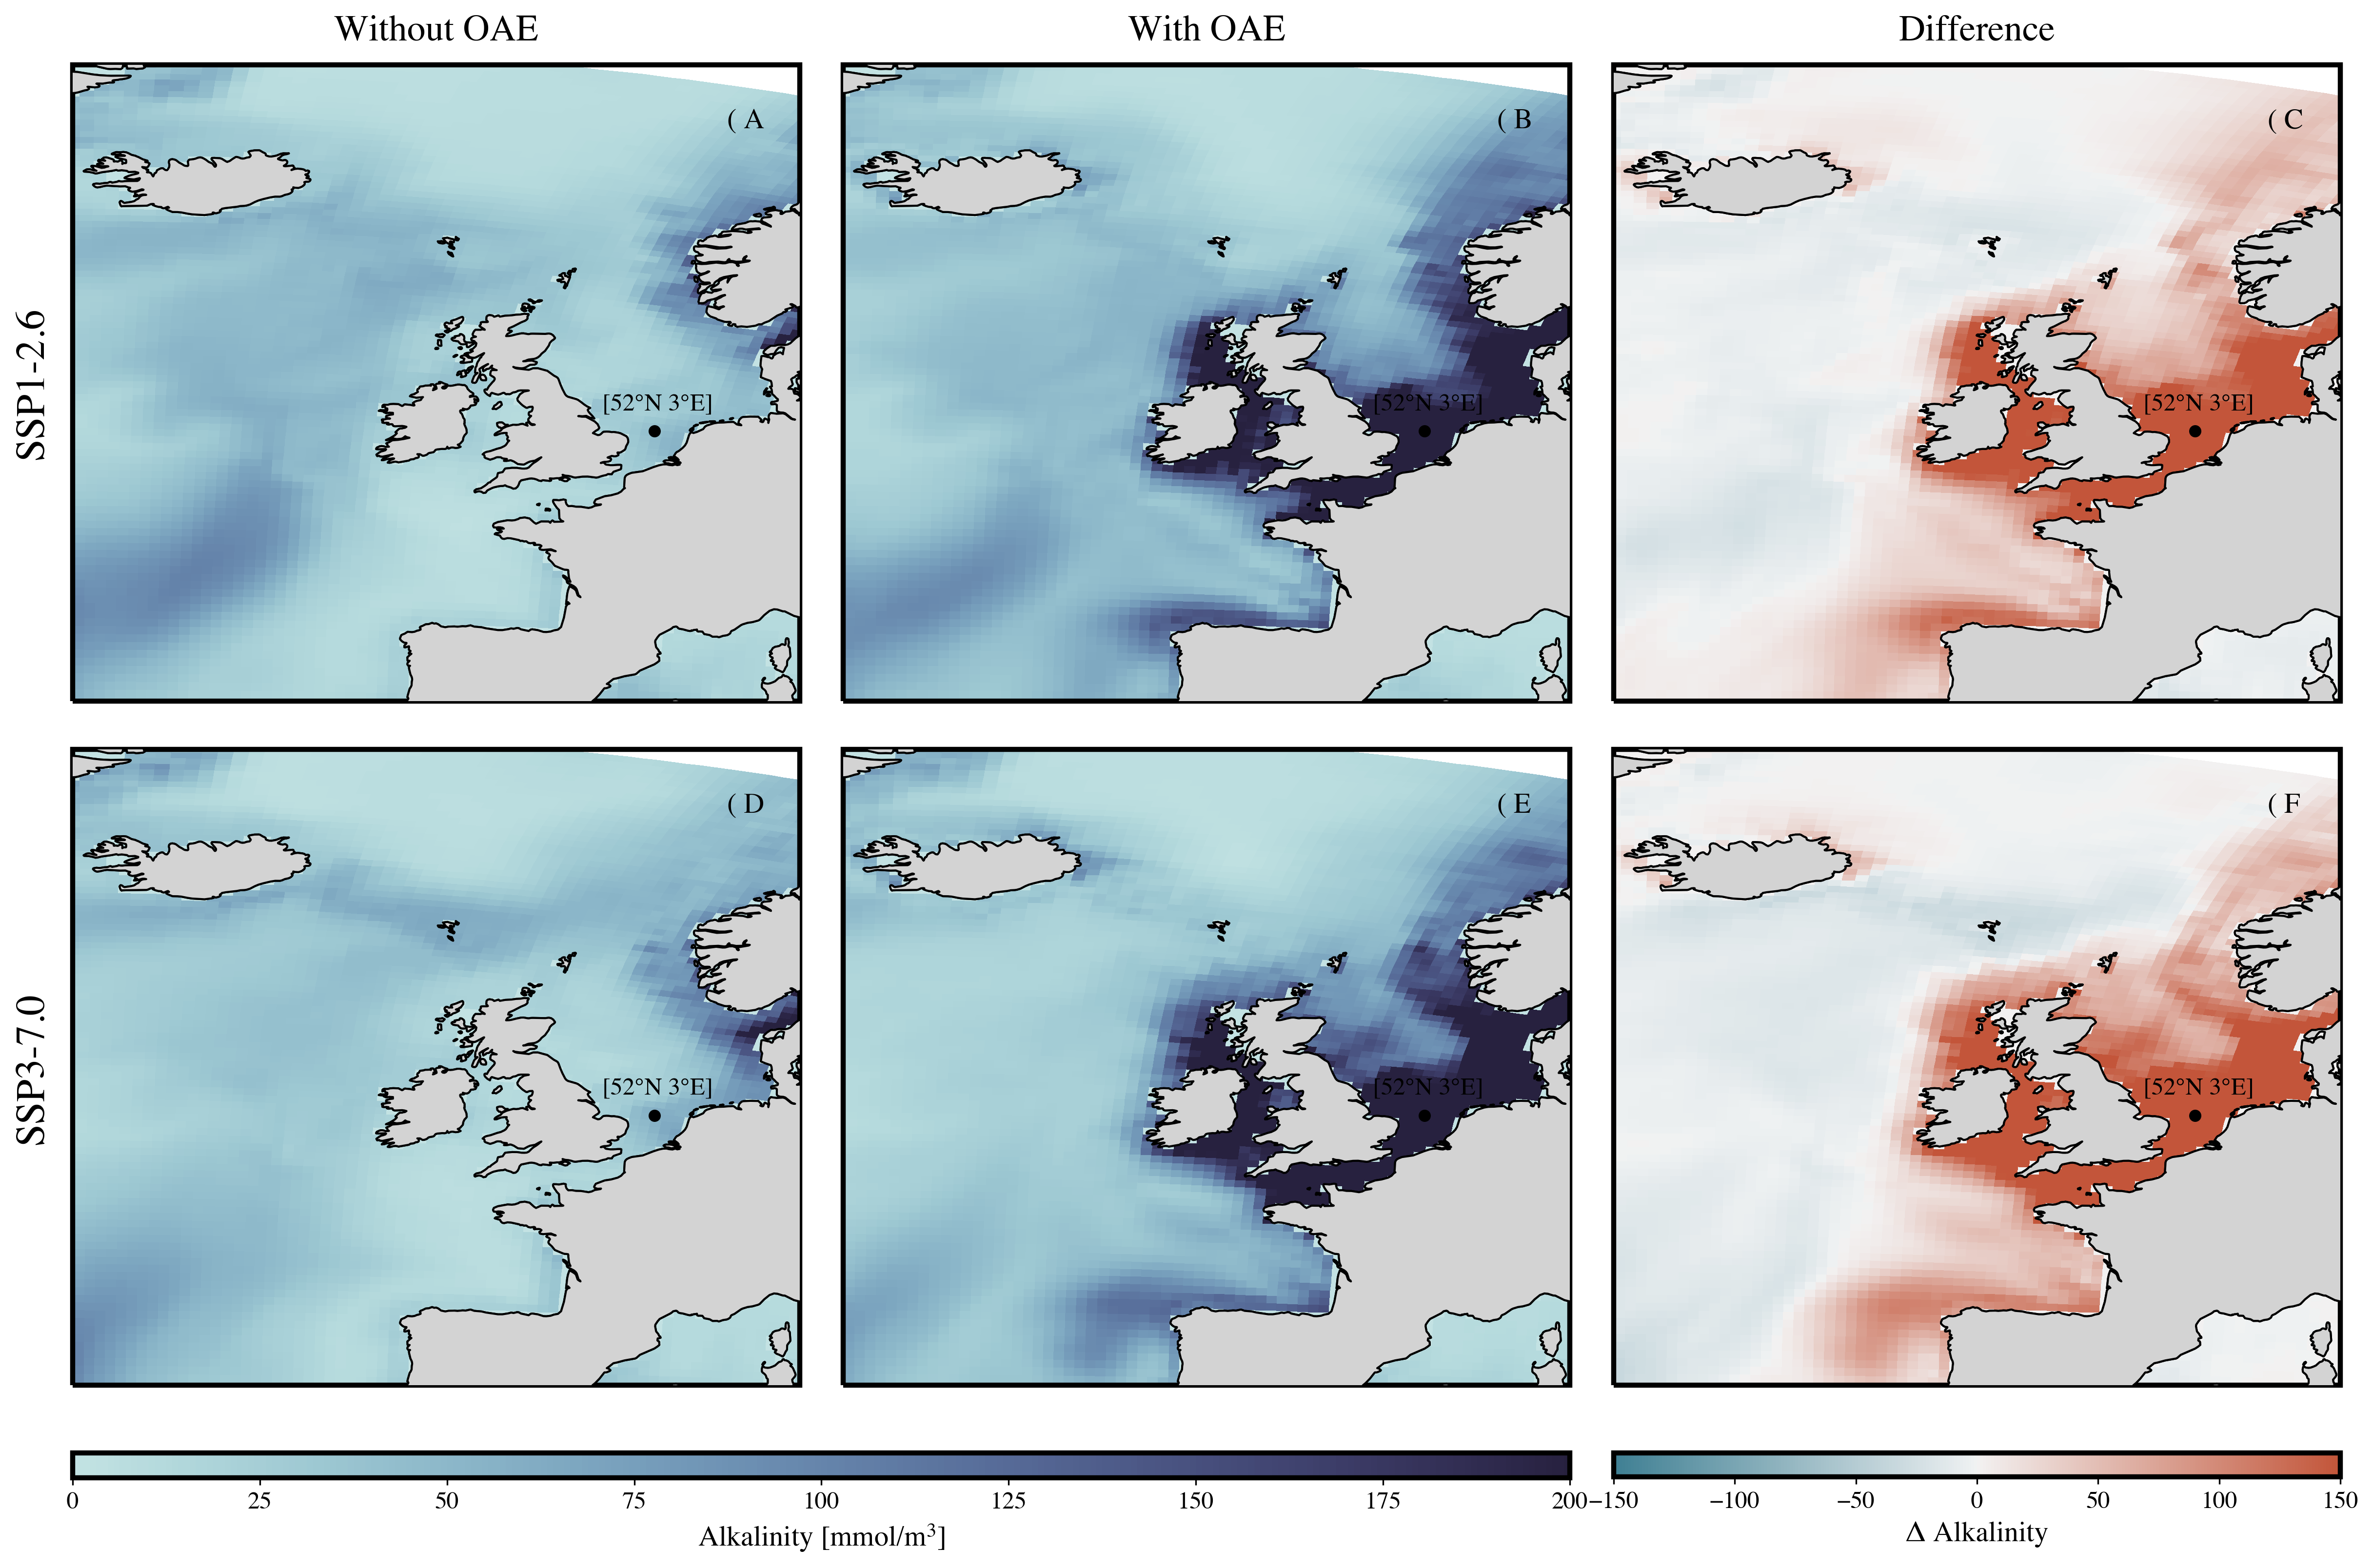
\includegraphics[width=15cm]{fig/3_Results/Alkalinity/alkalinity_ampl.png}

\end{figure}

In both scenarios, alkalinity addition operates to expand the seasonal amplitude only at the proximity of the injection site, especially at the UK littoral and in the southern and central North Sea (red regions in C and F of \cref{alkalinityamplitude}). The coasts of southern Norway and northern Spain represent an exception, where poor variation in amplitude is shown. Iceland reflects almost no change and its southern shoreline joins the pattern of the open ocean which displays a modest decreasing trend (light blue regions). In SSP3-7.0, the seasonal amplitude expands further than the low emission scenario, though maintaining the same pattern.

\section{pH:}

\begin{figure}[H]
\caption[Monthly average of baseline and \texorpdfstring{OAE}{OAE}-induced pH]{From left to right, monthly average of baseline and \ac{oae}-induced pH in the European region in SSP1-2.6 (A), and in SSP3-7.0 (C), and at location S in SSP1-2.6 (E) and in SSP3-7.0 (G) averaged over 2090-2100 (top), and the difference ($\Delta$) (B, D, F, and H) between the two scenarios (bottom).}
\label{ph}
\centering
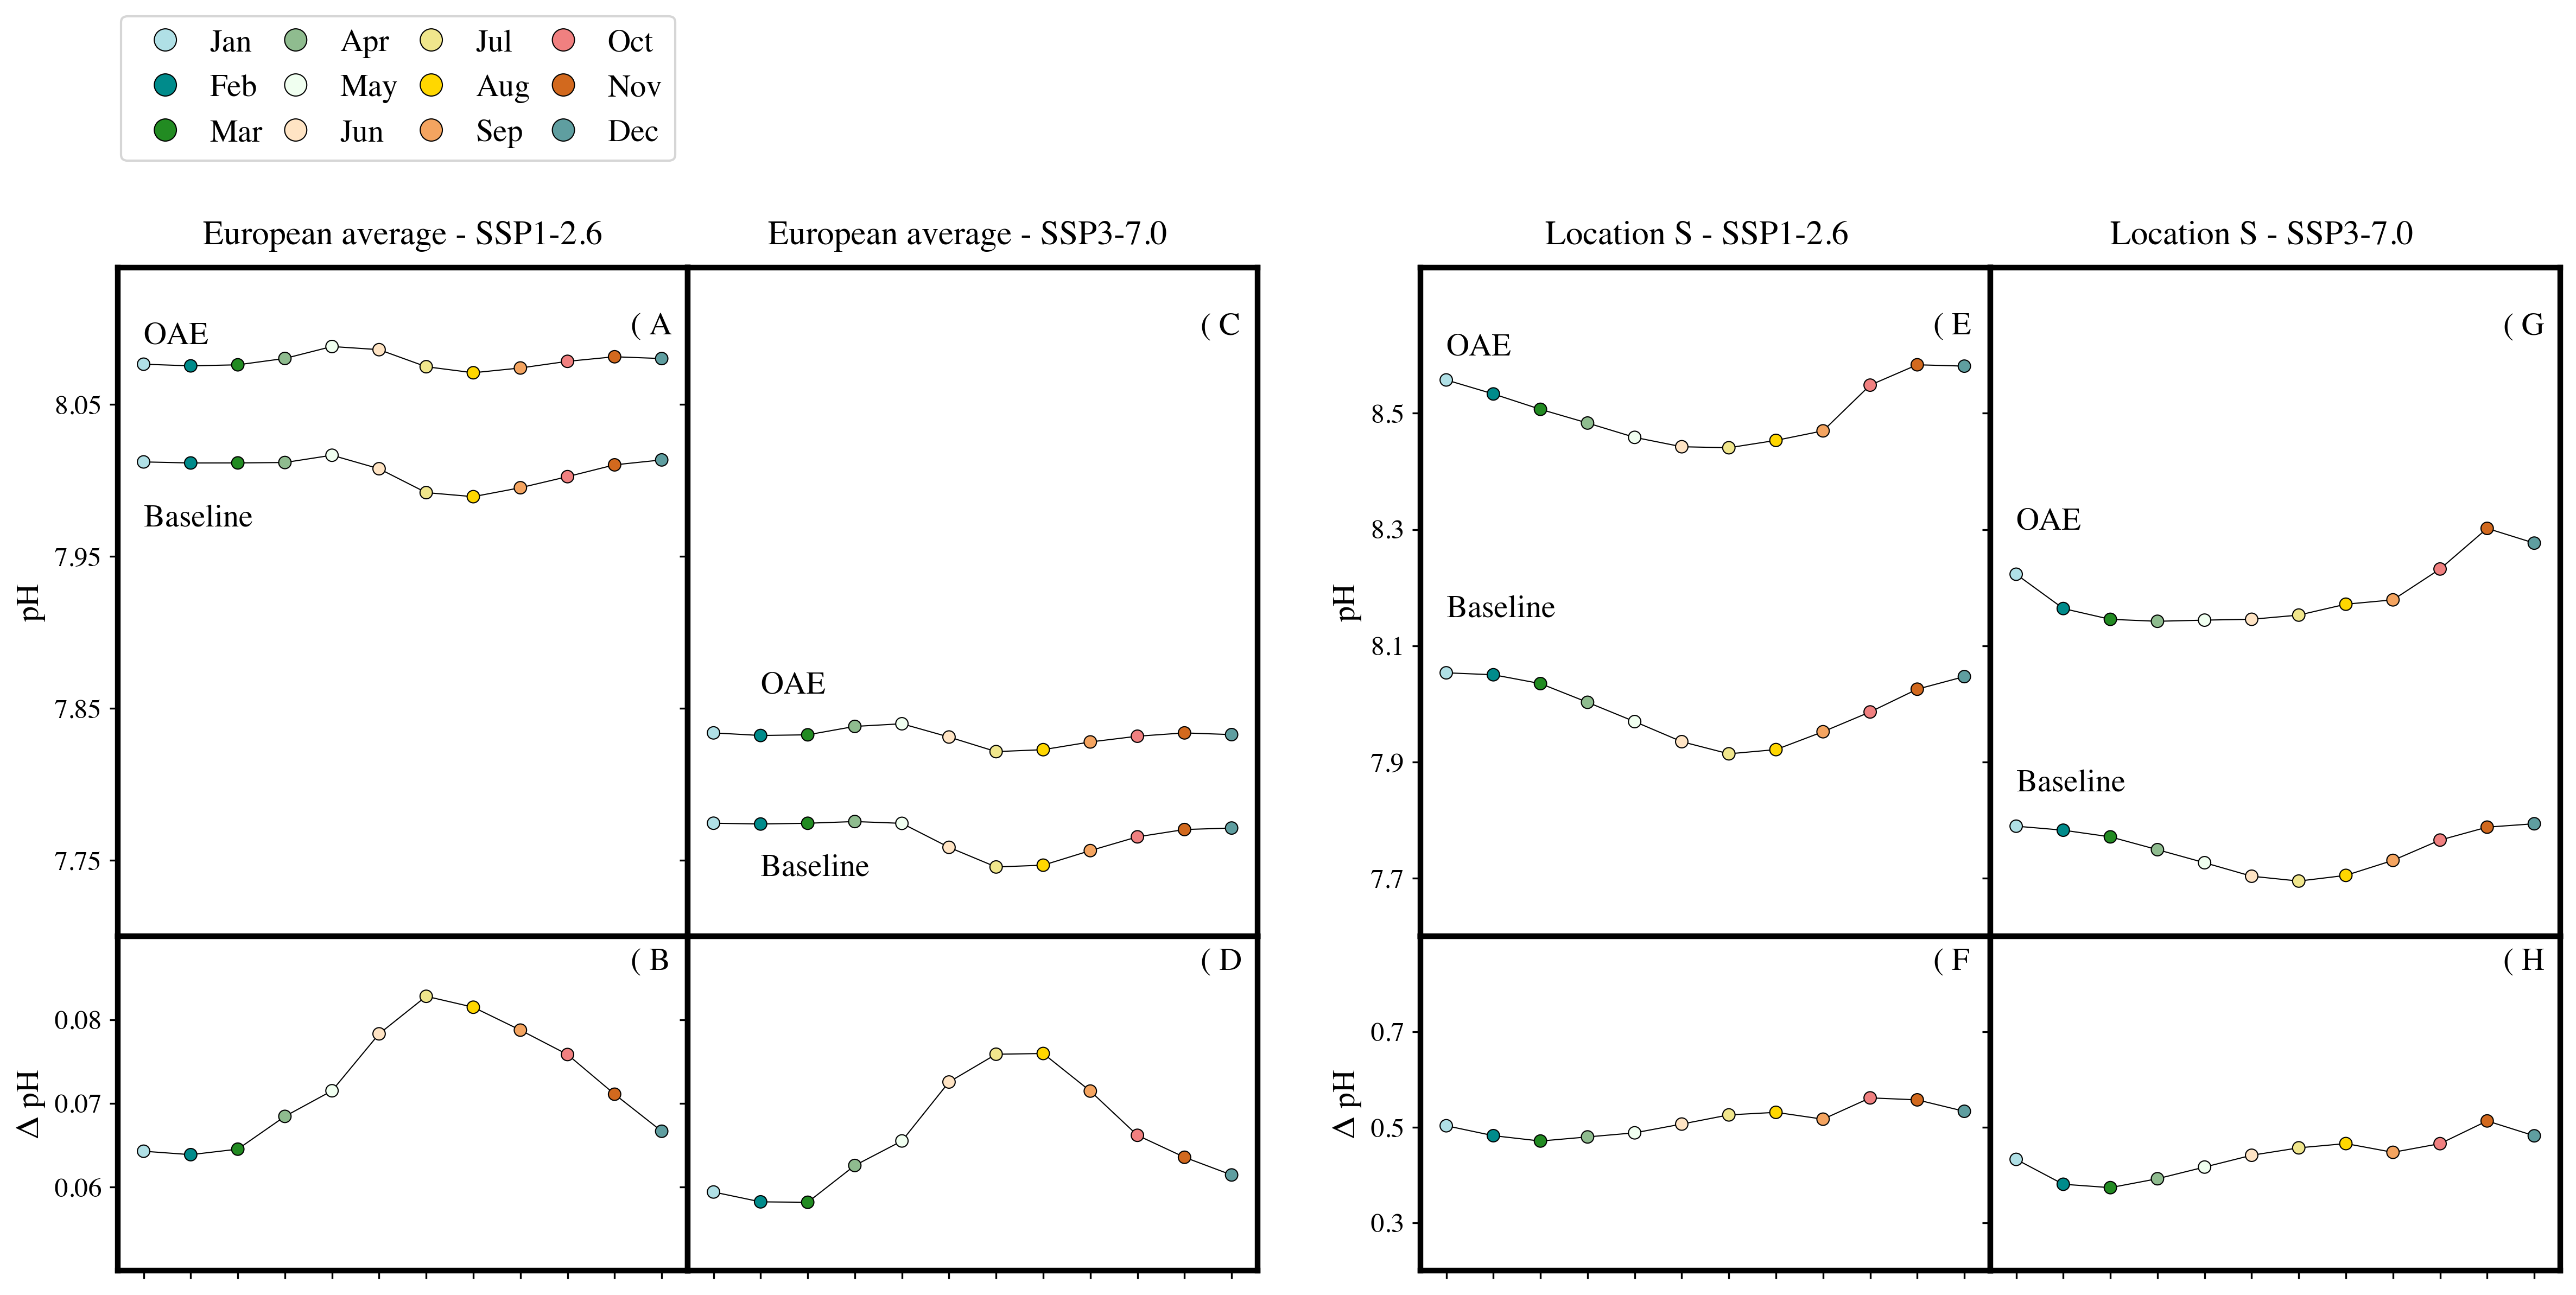
\includegraphics[width=15cm]{fig/3_Results/pH/ph.png}

\end{figure}

At the European average in SSP1-2.6, baseline pH reveals maxima in spring, reaching 8.01 units, and minima in summer, when it drops to 7.99. pH levels increase when \ac{oae} is employed and the amplitude is reduced by 0.01 units. This slight compression is due to \ac{oae} being most efficient at highest seawater acidification, that is, in summer months (B of \cref{ph}). In SSP3-7.0, pH absolute values are lower due to enhanced anthropogenic \ch{CO2} inputs to the atmosphere and a decreasing trend is registered until the end of the century (not shown). The seasonal amplitude change is maintained, with a minimal dampening compared to the baseline. 

At location S in SSP1-2.6, \ac{oae} is able to rise pH to values as high as over 8.5 units, with a nearly uniform increase throughout the year (F of \cref{ph}). In SSP3-7.0, \ac{oae} is able to restore pH levels, although not as efficiently as in the low-emission scenario. In both climate states, $\Delta$ pH reaches its peak in November, when highest alkalinity is detected (E and G of \cref{alkalinity}), showing a fast response to \ac{oae} perturbations. 

\begin{figure}[H]
\caption[pH seasonal amplitude change]{pH seasonal amplitude change without \ac{oae} (left), with \ac{oae} (middle), and the difference ($\Delta$) between the two (right). SSP1-2.6 (top) and SSP3-7.0 (bottom).}
\label{phamplitude}
\centering
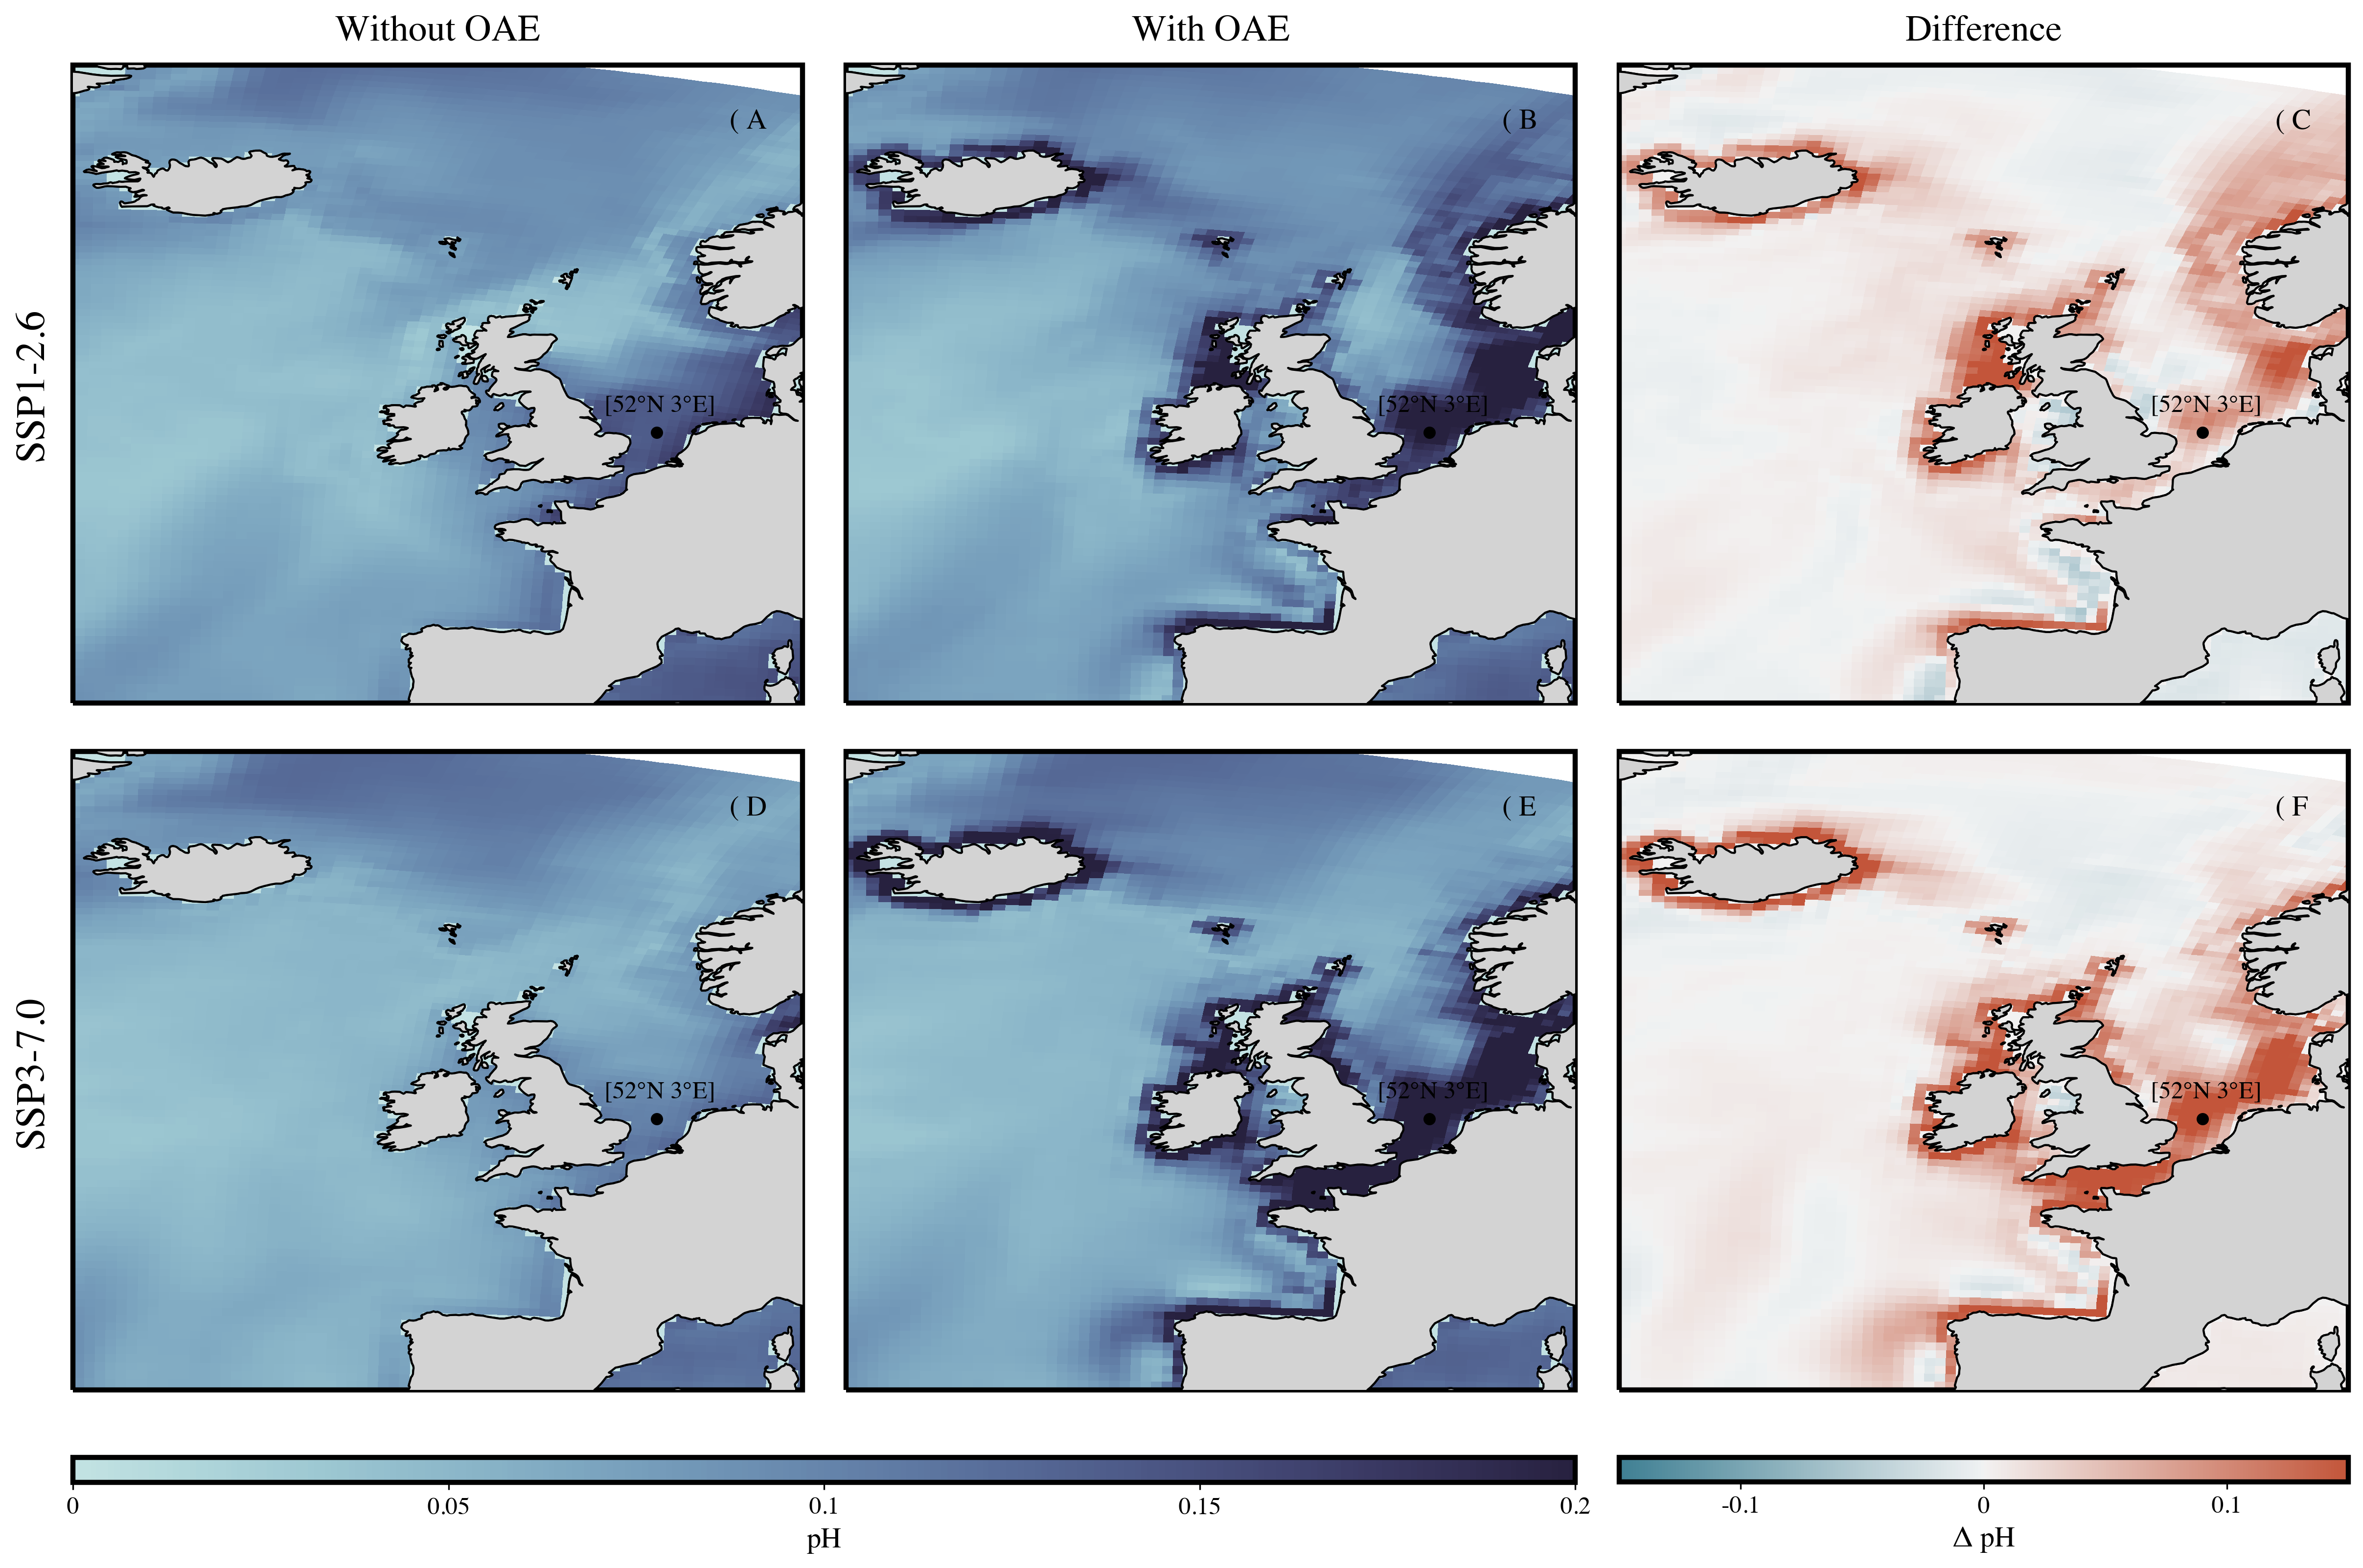
\includegraphics[width=15cm]{fig/3_Results/pH/ph_ampl.png}

\end{figure}

Modifications to the pH amplitude are not geographically homogeneous in SSP1-2.6 (top row in \cref{phamplitude}). In most of the European regions, pH seasonality expands, whereas a flattening is detected in the southern UK, western France and Spain (blue regions in C of \cref{phamplitude}). All changes are constrained to the vicinity of the coastline, where alkalinity addition was simulated. Under a higher-warming scenario, the pH seasonal amplitude cycle is better defined, showing that the entire European shore undergoes a strong increase in amplitude (red regions in F of \cref{phamplitude}). In both scenarios at open ocean, signals are mild or absent. 

\section[\texorpdfstring{DIC}{DIC}]{\ac{dic}:}

\begin{figure}[H]
\caption[Monthly average of baseline and \texorpdfstring{OAE}{OAE}-induced \texorpdfstring{DIC}{DIC}]{From left to right, monthly average of baseline and \ac{oae}-induced \ac{dic} (mmol m\textsuperscript{-3}) in the European region in SSP1-2.6 (A), and in SSP3-7.0 (C), and at location S in SSP1-2.6 (E) and in SSP3-7.0 (G) averaged over 2090-2100 (top), and the difference ($\Delta$) (B, D, F, and H) between the two scenarios (bottom).}
\label{dic}
\centering
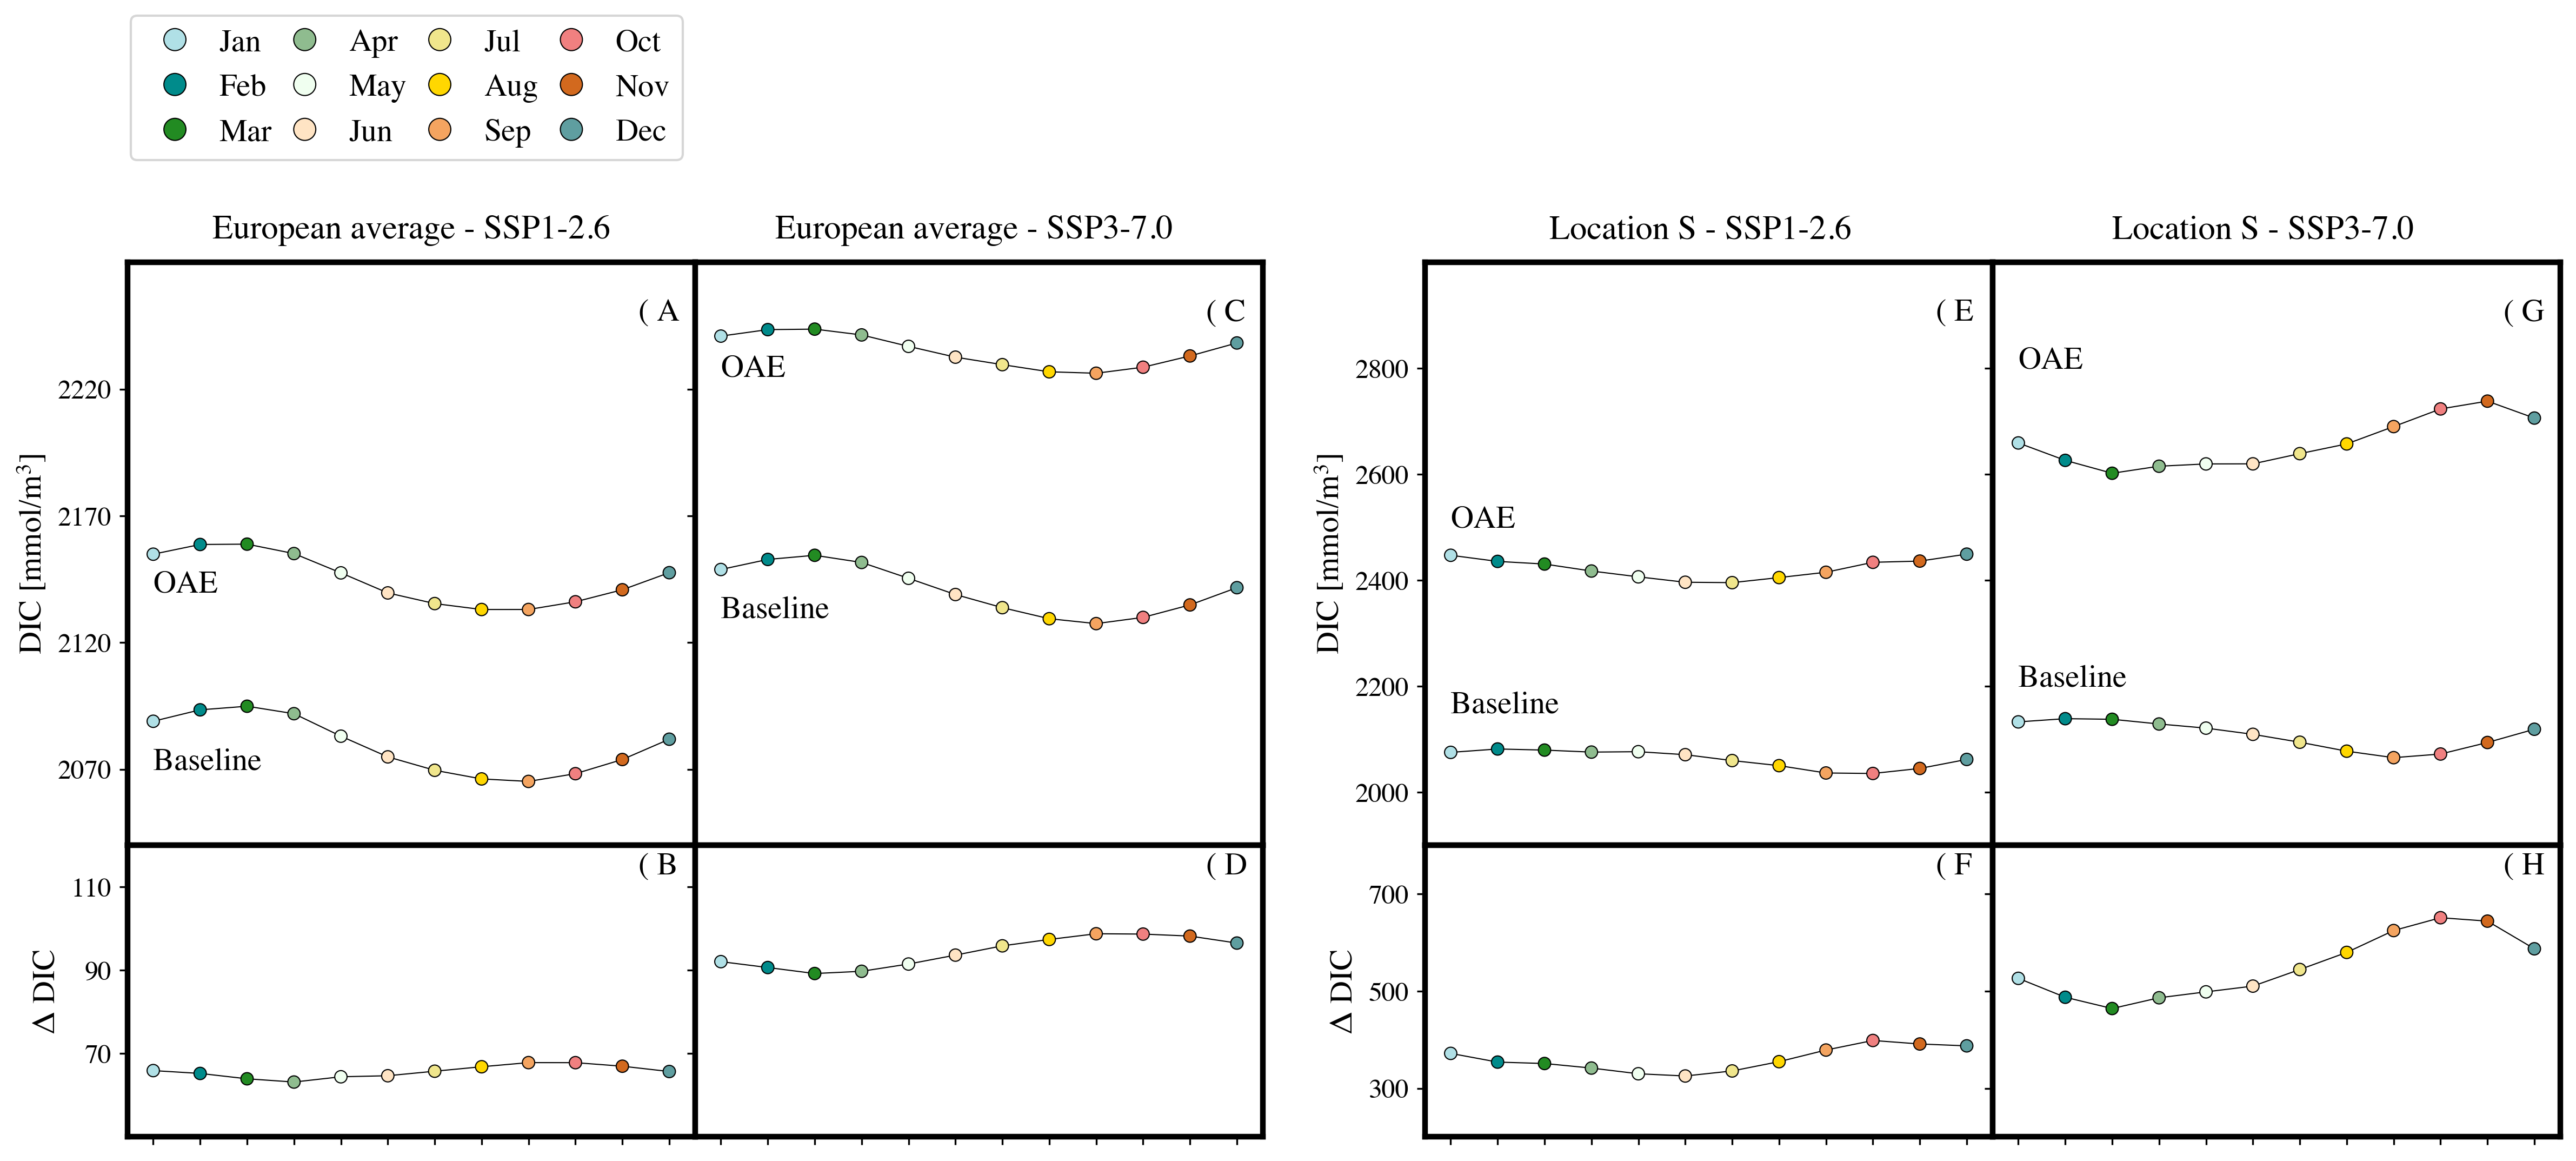
\includegraphics[width=15cm]{fig/3_Results/DIC/dic.png}

\end{figure}

In the European region in SSP1-2.6, \ac{dic} is characterised by highest and lowest levels in March and September, respectively. The average \ac{dic} seasonal cycle spans from 2065 to 2095 mmol m\textsuperscript{-3}. With \ac{oae} application, the \ac{dic} pool is significantly enhanced due to more \ch{CO2} input into the ocean but keeps reproducing the same seasonal pattern as the baseline. As for the amplitude, although minimal, a compression of 4 mmol m\textsuperscript{-3} is registered. Signal anomalies between scenarios are mainly detected between in autumn. In SSP3-7.0, \ac{dic} absolute values increase in response to rising atmospheric \ch{CO2} concentrations and consequent higher \ch{CO2} input into the ocean. D of \cref{dic} reveals that \ac{oae} is more efficient in driving \ac{dic} replenishment. 

At location S in SSP1-2.6, the ocean surface \ac{dic} is highest over the winter months and lowest in autumn. With \ac{oae}, minima are anticipated to the beginning of summer. The \ac{oae}-induced seasonal cycle stretches from 2396 to 2450 mmol m\textsuperscript{-3}. In SSP3-7.0, \ac{oae} forces the system to a shift. Carbon content increases at the ocean surface in November whereas undersaturation takes place especially in March, where the curve begins rising again. This describes a meaningful seasonal alteration from the baseline. The current cycle spans from 2602 to 2738 mmol m\textsuperscript{-3}. Both $\Delta$ \ac{dic} of SSP3-7.0 (D and H of \cref{dic}) show a larger baseline-to-\ac{oae} anomaly than their respective SSP1-2.6.

\begin{figure}[H]
\caption[\texorpdfstring{DIC}{DIC} seasonal amplitude change]{\ac{dic} seasonal amplitude change (mmol m\textsuperscript{-3}) without \ac{oae} (left), with \ac{oae} (middle), and the difference ($\Delta$) between the two (right). SSP1-2.6 (top) and SSP3-7.0 (bottom).}
\label{dicamplitude}
\centering
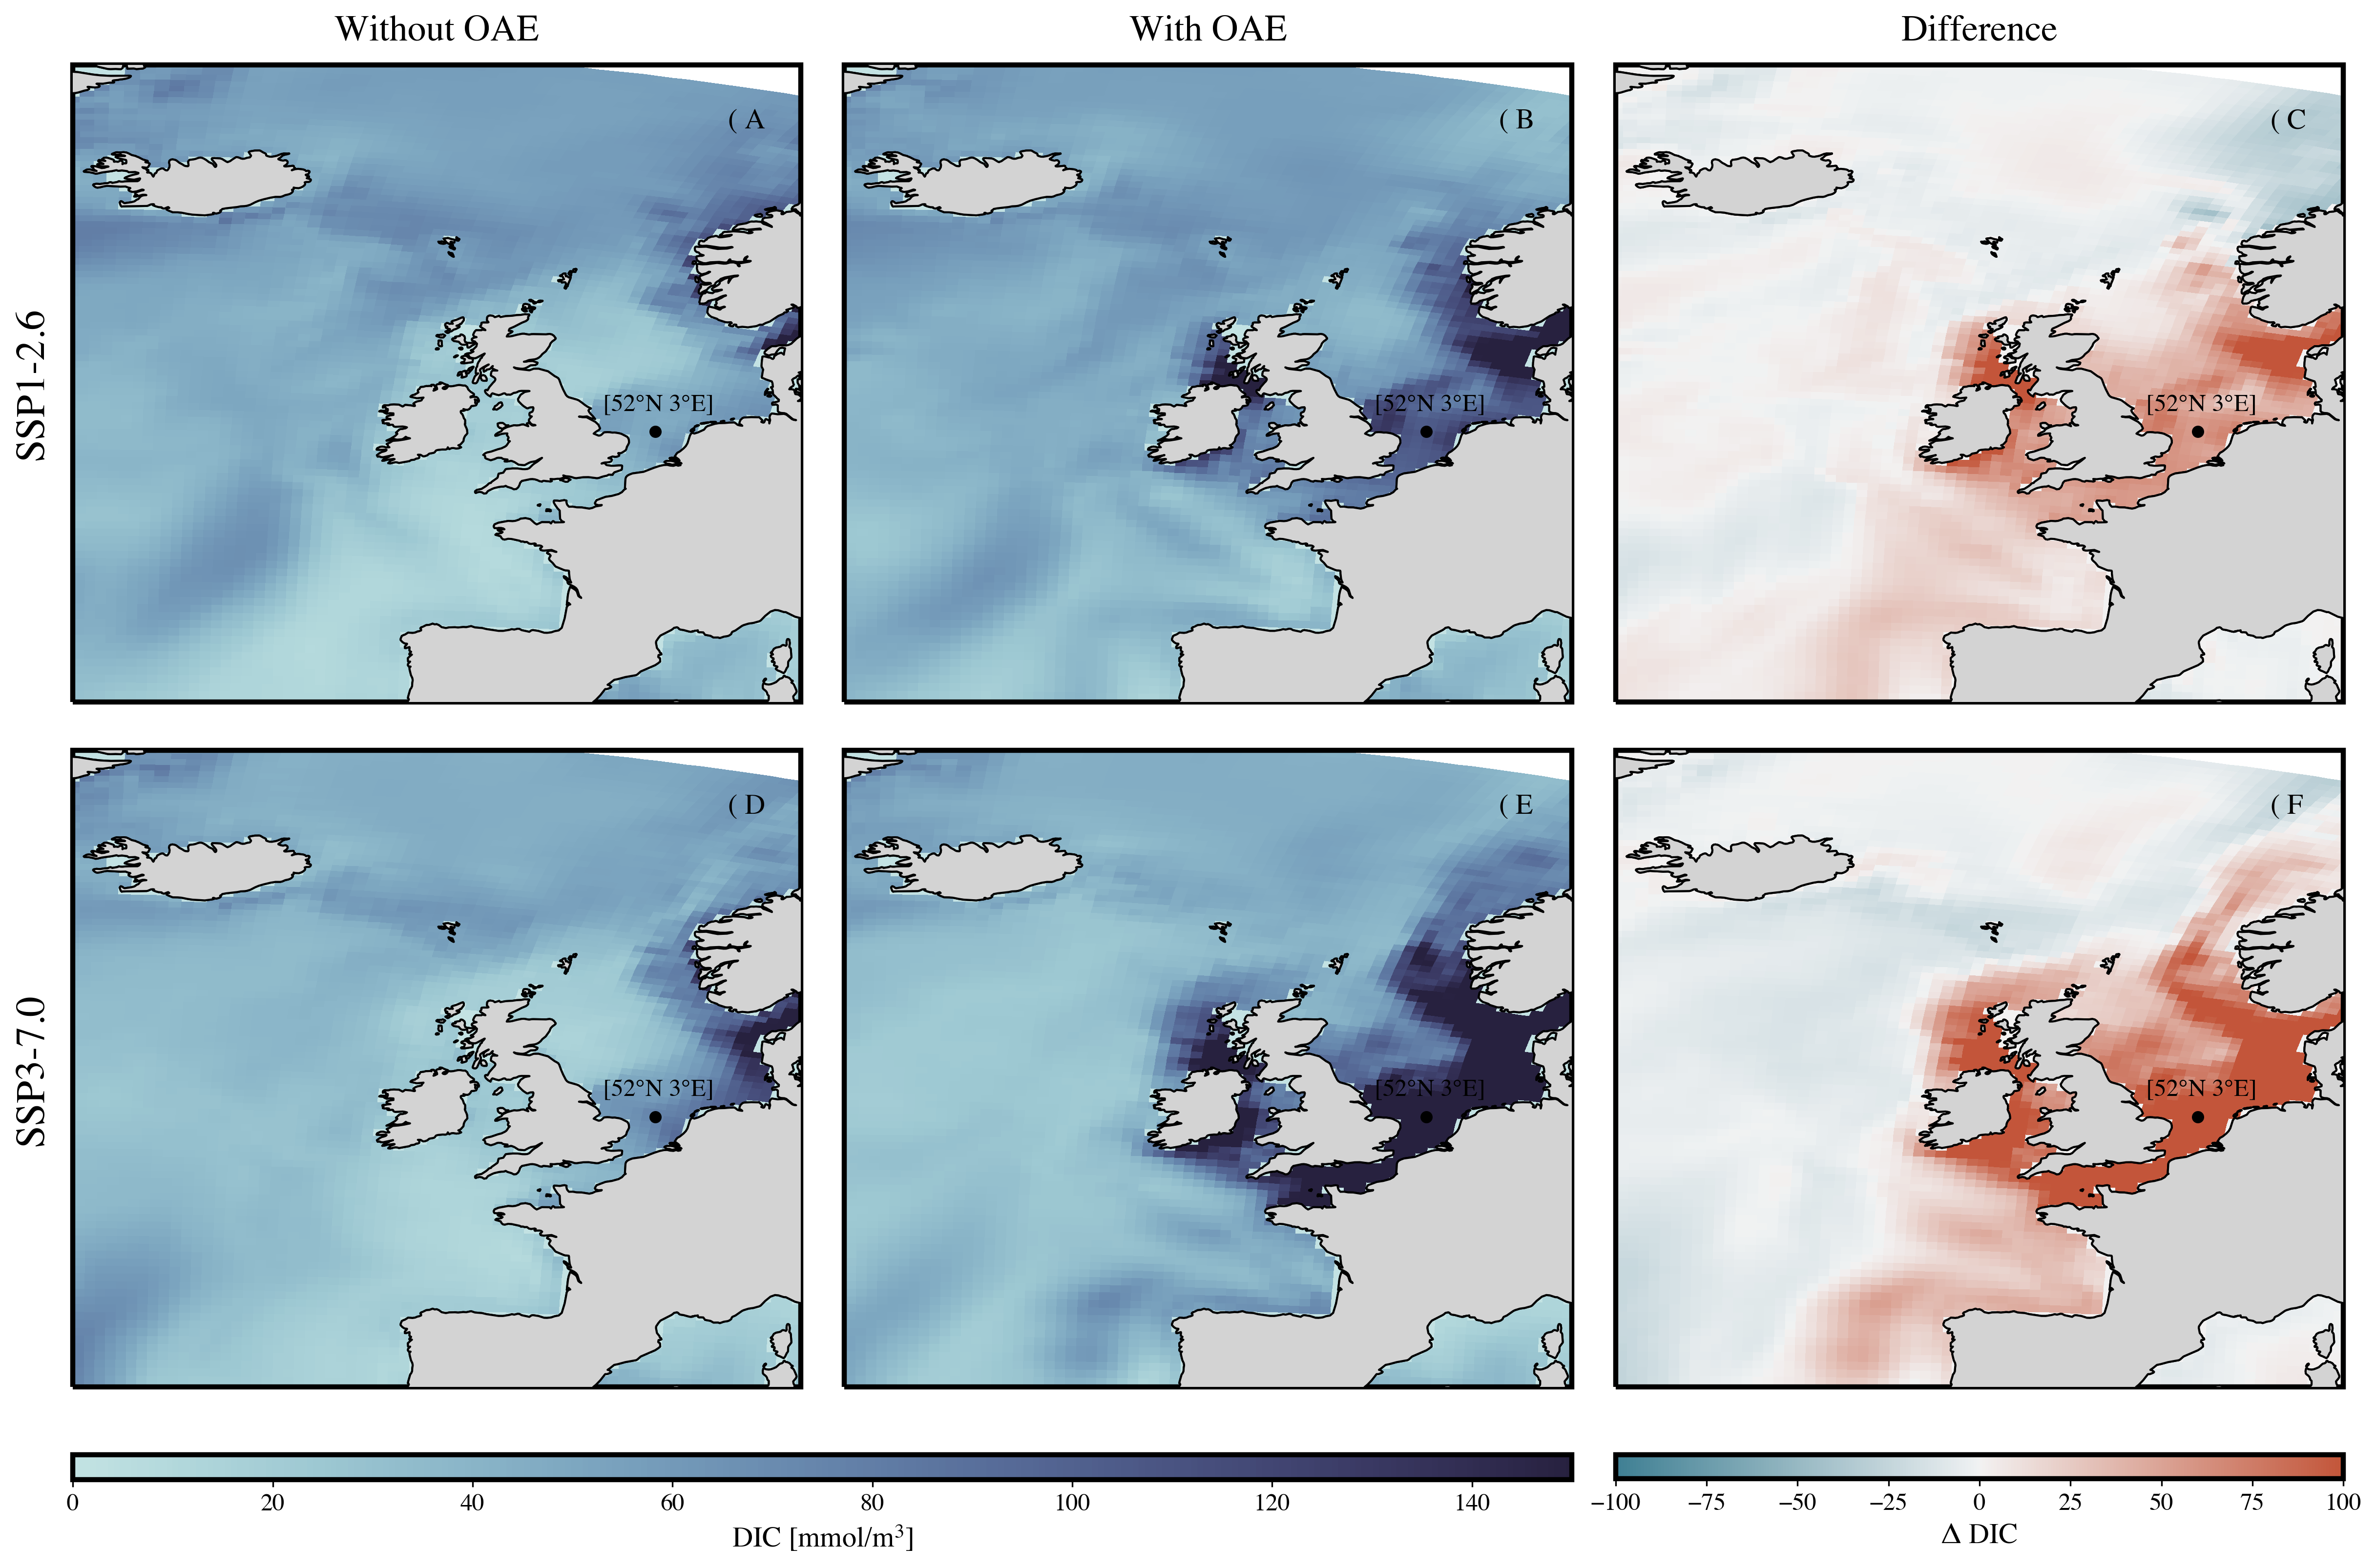
\includegraphics[width=15cm]{fig/3_Results/DIC/dic_amplitude.png}

\end{figure}

In SSP1-2.6, the most pronounced \ac{dic} seasonal amplification is observed only at two locations: off of the coasts of northern Northern Ireland and in the Skagerrak sea (dark red regions in C of \cref{dicamplitude}). A less acute seasonal amplification is still detected in the southern and central North Sea whereas, at open ocean, no propagation occurs and most regions remain overall unaffected. In SSP3-7.0, the \ac{dic} seasonal cycle is much more amplified with respect to the baseline, although confined to the partly enclosed North Sea and the UK coastline. Mild amplification is observed by the Spanish and Norwegian banks. 

\section{Ocean \ch{pCO2}:}

\begin{figure}[H]
\caption[Monthly average of baseline and \texorpdfstring{OAE}{OAE}-induced ocean \ch{pCO2}]{From left to right, monthly average of baseline and \ac{oae}-induced ocean \ch{pCO2} (µatm) in the European region in SSP1-2.6 (A), and in SSP3-7.0 (C), and at location S in SSP1-2.6 (E) and in SSP3-7.0 (G) averaged over 2090-2100 (top), and the difference ($\Delta$) (B, D, F, and H) between the two scenarios (bottom).}
\label{fco2}
\centering
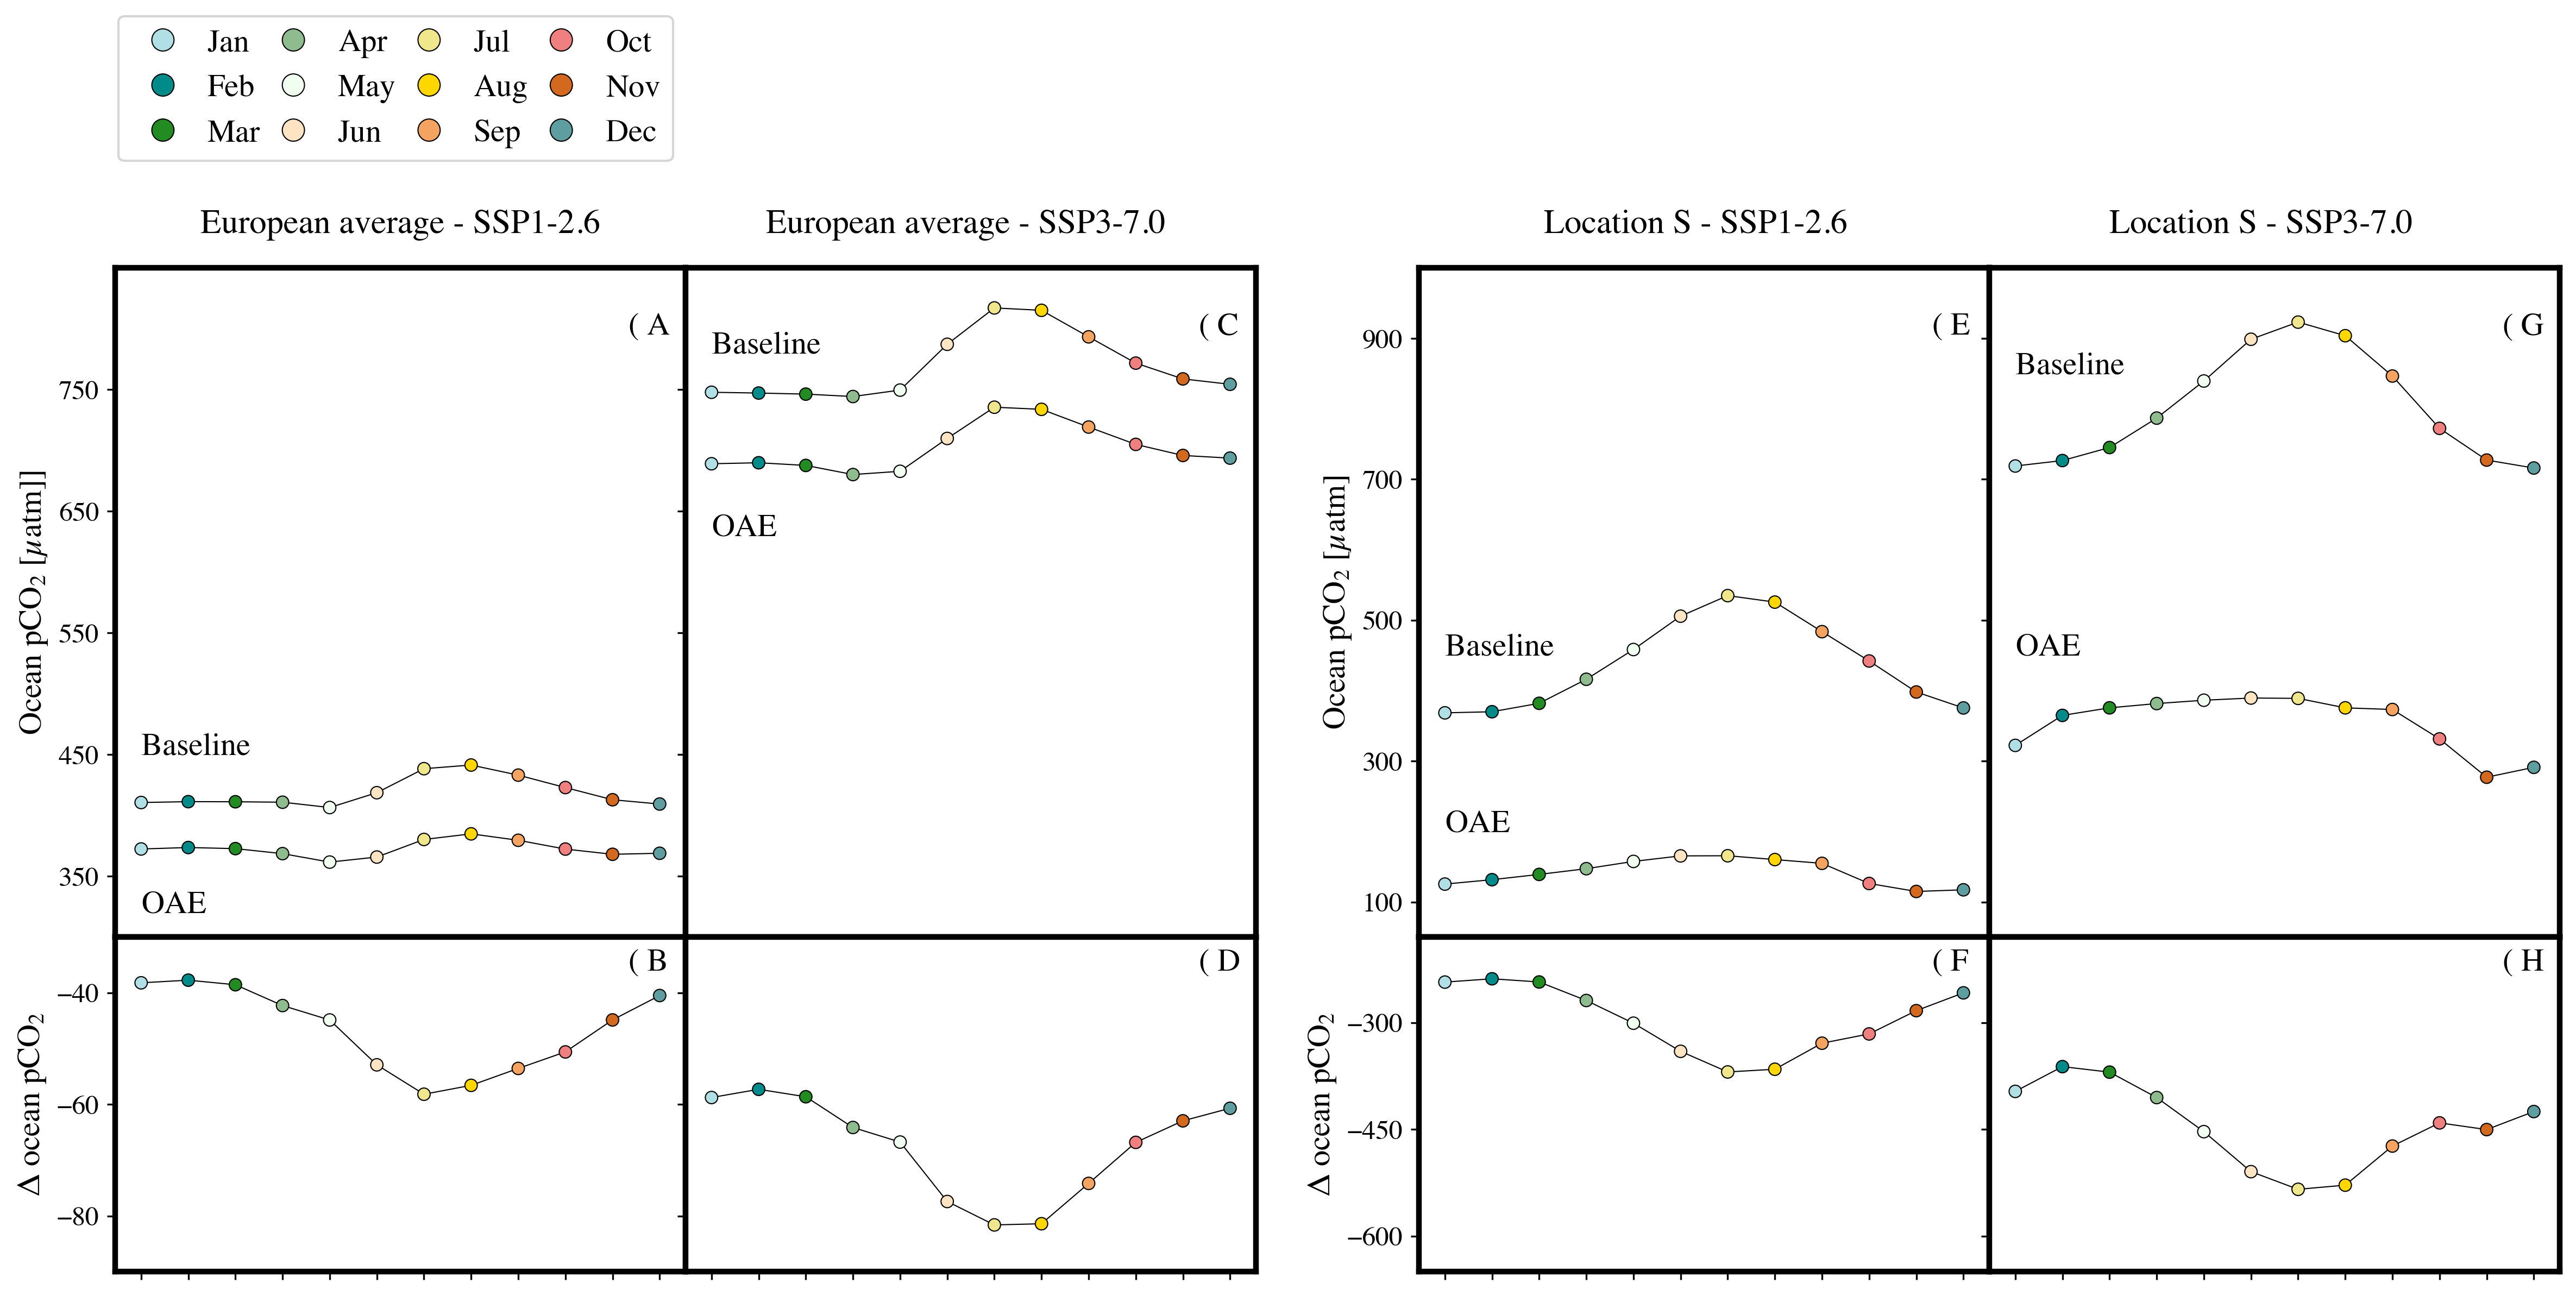
\includegraphics[width=15cm]{fig/3_Results/pCO2/fco2.png}

\end{figure}

In the European region in SSP1-2.6, ocean \ch{pCO2} is characterised by least and most elevated values in May and August, respectively, with a mean amplitude stretching from 407 to 441 µatm. In the \ac{oae} scenario, \ch{CO2} partial pressure is reduced due to alkalinity enhancement and \ch{pCO2} absolute values drop, now spanning between 362 and 385 µatm. The seasonal amplitude of the \ac{oae} scenario is therefore depressed. $\Delta$ \ch{pCO2} detects the largest anomalies between the two scenarios in summer (B of \cref{fco2}), signifying that alkalinity encourages \ch{pCO2} decline when \ch{CO2} outgassing takes place. In SSP3-7.0 baseline, \ch{pCO2} maintains an ascending trend until 2100 (not shown). Seasonally, elevated values are recorded in July and then decline until minima are reached in April. The mean seasonality has highest and lowest peaks of 817 and 744 µatm, respectively. In C of \cref{fco2}, it is evident that \ac{oae} induces the cycle to decrease substantially, with an amplitude of 55 µatm. 

Unlike the European average, location S displays minima in winter, denoting that \ch{pCO2} decrease is here anticipated. Predictably, \ac{oae} reduces \ch{pCO2} absolute values. The seasonal amplitude is compressed to less than a third compared to the baseline, with an average span of 51 µatm. $\Delta$ \ch{pCO2} oscillates between winter lows and summer highs, as \ac{oae} primarily helps to weaken the ocean pressure that encourages \ch{CO2} to escape. In SSP3-7.0, the baseline has a seasonal amplitude ranging between 716 and 923 µatm. Alkalinity addition causes \ch{pCO2} to drop substantially. Its seasonal cycle is also compressed and stays between 277 and 390 µatm. $\Delta$ \ch{pCO2} confirms that the largest discrepancy takes place in summer, at highest ocean \ch{pCO2} (H of \cref{fco2}). 

\begin{figure}[H]
\caption[\ch{pCO2} seasonal amplitude change]{\ch{pCO2} seasonal amplitude change (µatm) without \ac{oae} (left), with \ac{oae} (middle), and the difference ($\Delta$) between the two (right). SSP1-2.6 (top) and SSP3-7.0 (bottom).}
\label{pco2amplitude}
\centering
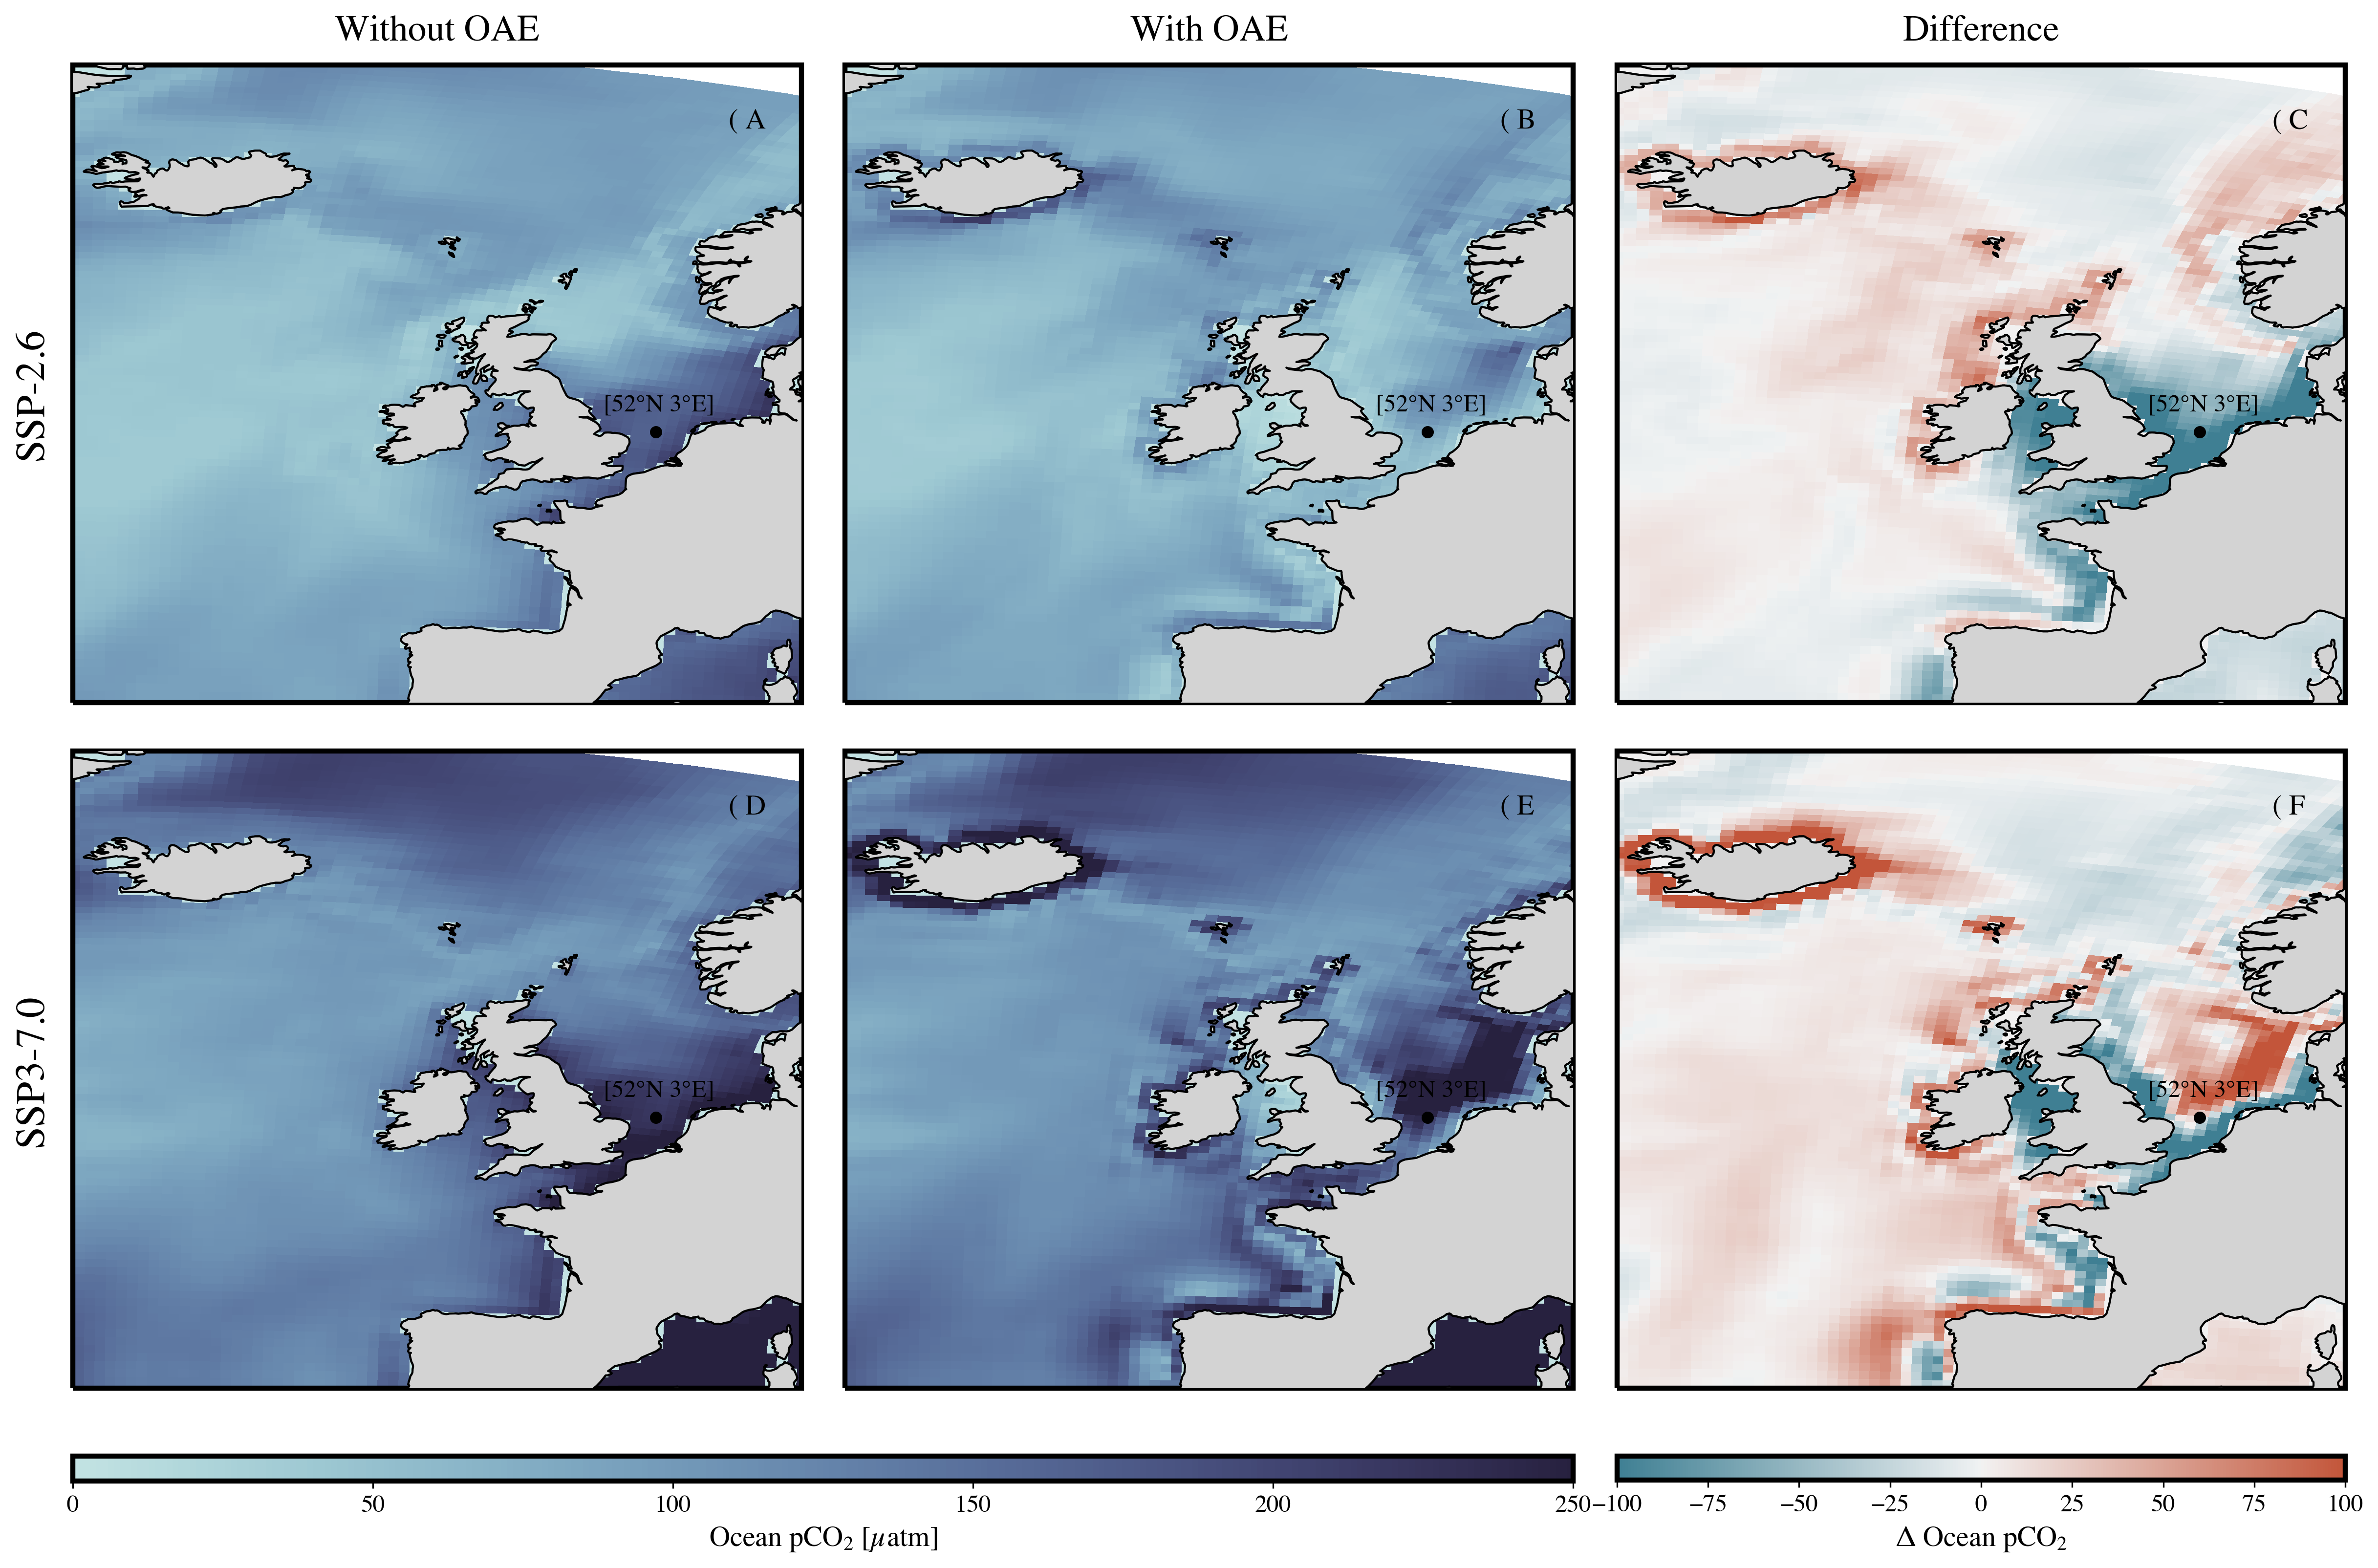
\includegraphics[width=15cm]{fig/3_Results/pCO2/fco2_ampl.png}

\end{figure}

In \cref{pco2amplitude} for SSP1-2.6, a clear pattern is identified at the proximity of the injection location, with two diverging geographies. At higher latitudes, in Iceland, the Norwegian, the Spanish North and the British North-West bank, \ch{pCO2} seasonal amplitude is slightly more pronounced than the baseline (red regions in C of \ref{pco2amplitude}). Conversely, at lower latitudes including the mainland shore and the central-to-southern UK coasts, \ch{pCO2} seasonal breadth is strongly mitigated (blue regions). In SSP3-7.0, \ch{pCO2} amplitude behaves similarly, with the exception of the centre-to-north North Sea and northern Spain, where strong amplification is displayed. At open sea, \ch{pCO2} seasonality is slightly amplified in the North Atlantic and dampened in the sub-polar regions.

\section{\ch{CO2} flux:}

\begin{figure}[H]
\caption[Monthly average of baseline and \texorpdfstring{OAE}{OAE}-induced ocean \ch{CO2} flux]{From left to right, monthly average of baseline and \ac{oae}-induced ocean \ch{CO2} (mmol/m\textsuperscript{2}/yr) in the European region in SSP1-2.6 (A), and in SSP3-7.0 (C), and at location S in SSP1-2.6 (E) and in SSP3-7.0 (G) averaged over 2090-2100 (top), and the difference ($\Delta$) (B, D, F, and H) between the two scenarios (bottom). Negative values represent \ch{CO2} uptake by the ocean.}
\label{co2flux}
\centering
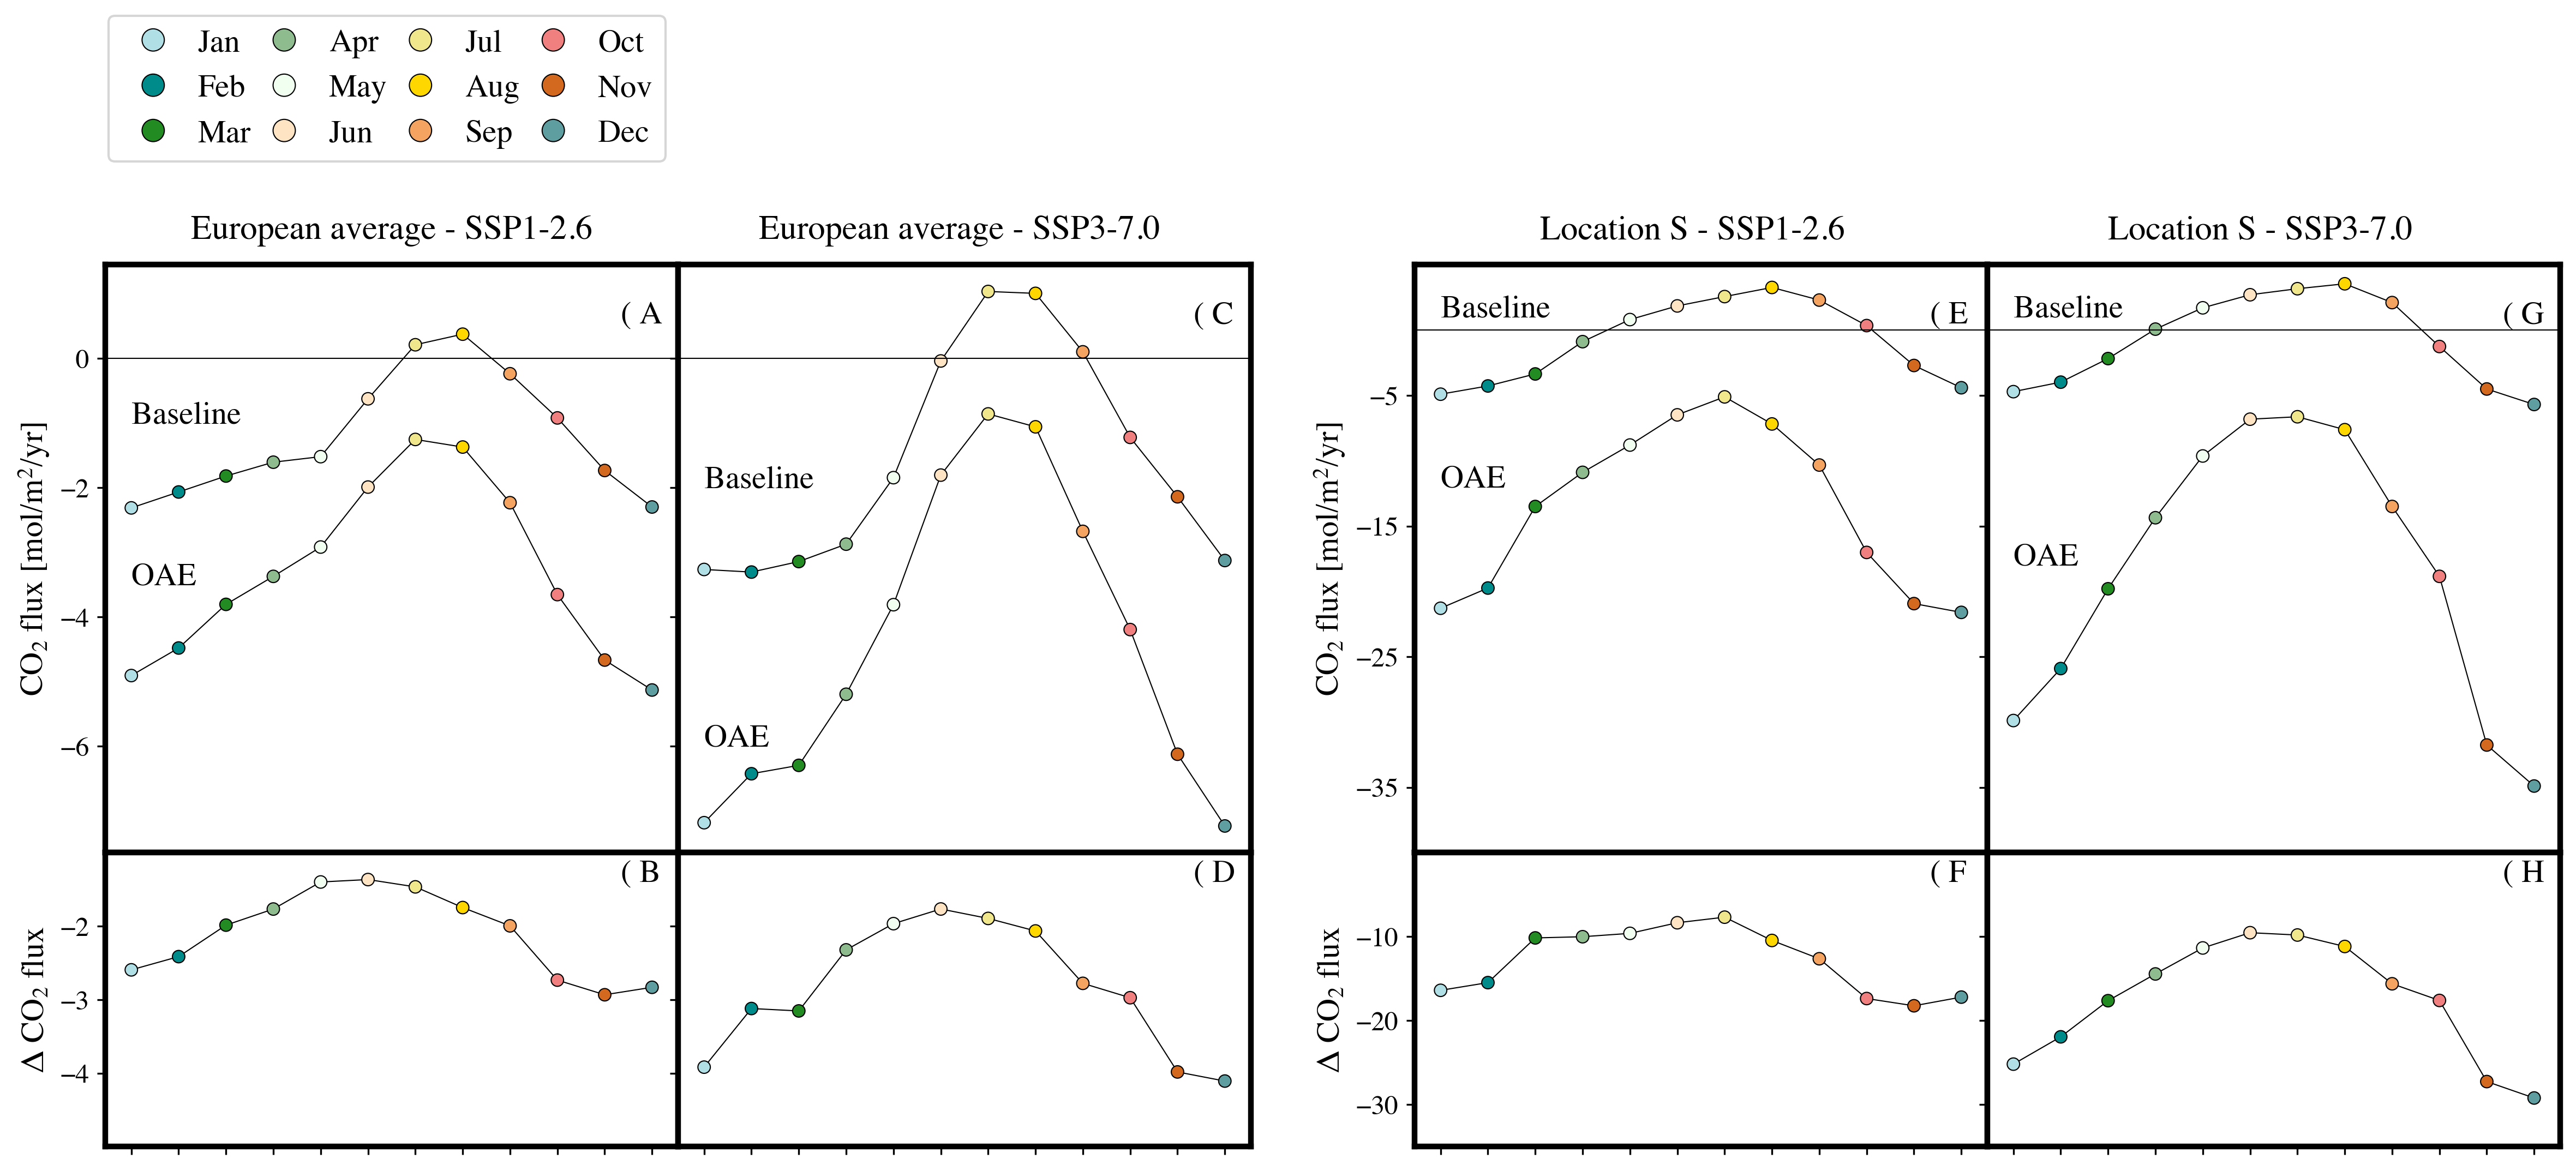
\includegraphics[width=15cm]{fig/3_Results/CO2flux/co2flux.png}

\end{figure}

A of \cref{co2flux} shows that, at the European average in SSP1-2.6, the baseline ocean tends to outgass \ch{CO2} in summer (in July and August), while remaining a carbon sink over the rest of the year, with most pronounced uptake in winter, especially December. This outcome agrees with \ac{dic} seasonality, where winter uptake enhances the \ac{dic} pool and summer outgassing depletes it. When \ac{oae} is applied, the system is turned into a sink all year round, with summertime (wintertime) reflecting the least (most) \ch{CO2} uptake. Following the baseline, it is in July and January that extremes are detected. The seasonal amplitude varies noticeably, with the \ac{oae} scenario showing a much greater breadth than the baseline. \ch{CO2} flux amplitude has now an average span of -1.25 to -5.12, compared to the baseline that stayed between 0.37 and -2.31 mol m\textsuperscript{-2} yr\textsuperscript{-1}. In SSP3-7.0, the baseline outgasses \ch{CO2} from July to September. Adding alkalinity increases the \ch{CO2} seasonal amplitude more than the low emission scenario, especially in winter where minima $\Delta$ \ch{CO2} flux are observed. 

In the baseline of both scenarios at location S, \ch{CO2} flux reflects a downward flow in colder months and an upward flow in warmer months, splitting the annual cycle into two equally long phases. Outgassing happens from May to September/October and uptake from November to March/April, on average. In \ac{oae}-induced SSP1-2.6, \ch{CO2} flux fluctuates between -21.6 and -5.11 mol m\textsuperscript{-2} yr\textsuperscript{-1} on average, therefore doubling the baseline amplitude. Seasonality of \ch{CO2} flux in SSP3-7.0 is considerably enhanced when alkalinity is added, with a current amplitude of 28 mol m\textsuperscript{-2} yr\textsuperscript{-1}, three times larger than the baseline. In B, D, F, and H of \cref{co2flux}, the baseline-to-\ac{oae} discrepancies grow in winter and drop in summer, meaning that the impacts of alkalinisation on the ocean surface are largest when ocean uptake is already most pronounced. \ac{oae}-induced changes on the \ch{CO2} flux are disproportionately higher in winter, meaning that lower lows are not compensated for by equally higher highs.

\begin{figure}[H]
\caption[\ch{CO2} flux seasonal amplitude change]{\ch{CO2} flux seasonal amplitude change (mol m\textsuperscript{-2} yr\textsuperscript{-1}) without \ac{oae} (left), with \ac{oae} (centre), and the difference ($\Delta$) between the two (right). SSP1-2.6 (top) and SSP3-7.0 (bottom).}
\label{co2fluxamplitude}
\centering
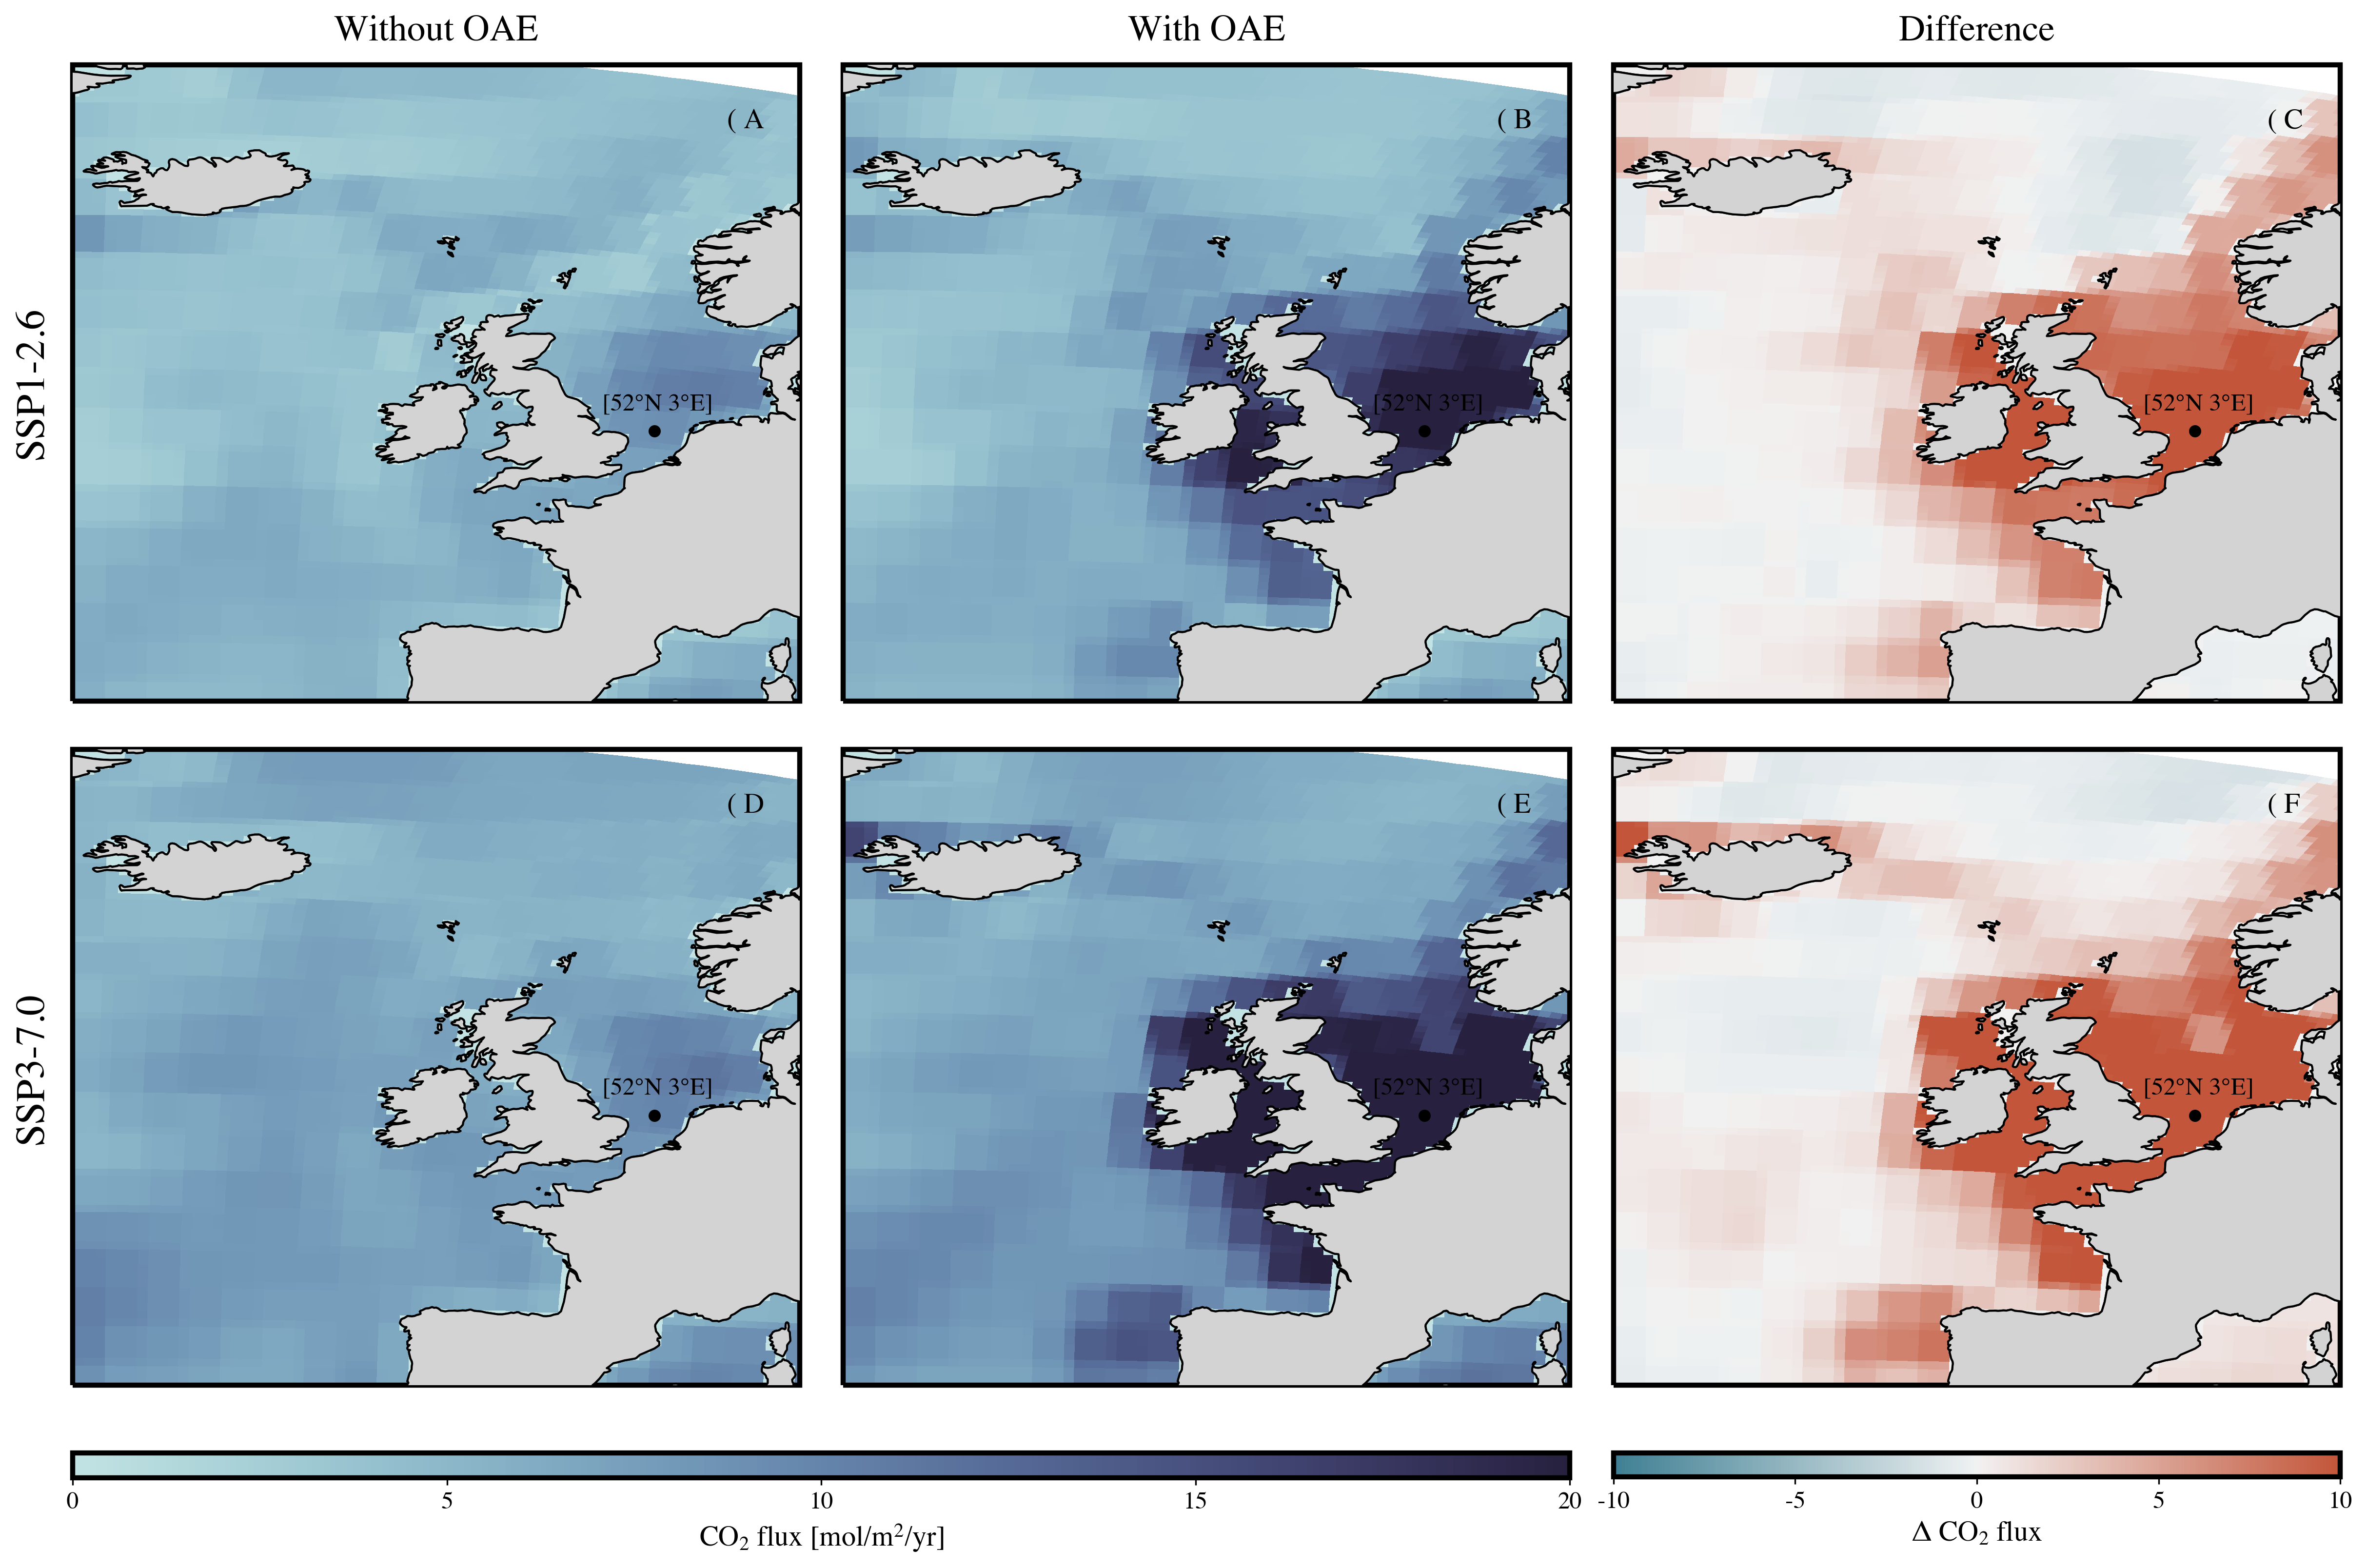
\includegraphics[width=15cm]{fig/3_Results/CO2flux/co2flux_ampl.png}

\end{figure}

With \ac{oae}, SSP1-2.6 in \cref{co2fluxamplitude} reveals an increase in \ch{CO2} seasonal fluxes along the European coasts, especially in the partially enclosed system of the southern North Sea and western UK coasts (red regions in C of \cref{co2fluxamplitude}. Poor-to-no changes are observed in Iceland, Spain and Norway. SSP3-7.0 mirrors the same spatial pattern as SSP1-2.6. When \ac{oae} is implemented, a system shift induces a seasonal cycle amplification in the proximity of the injection line. Largest modifications are detected in the southern North Sea. Overall, a higher emission scenario results in a magnification of the SSP1-2.6 variations. Geographically, in both SSP1-2.6 and SSP3-7, it is noted that \ch{CO2} seasonal amplitude modifications are registered well beyond where modulations associated to the other variables are detected, although signals at open ocean remain absent. 

\subsection[\texorpdfstring{OAE}{OAE}-induced carbon uptake potential:]{\ac{oae}-induced carbon uptake potential:}

\begin{figure}[H]
\caption[\texorpdfstring{OAE}{OAE}-induced change in carbon inventory]{\ac{oae}-induced change in carbon inventory in SSP1-2.6 (left) and SSP3-7.0 (right) over 2090-2100.}
\label{cgt}
\centering
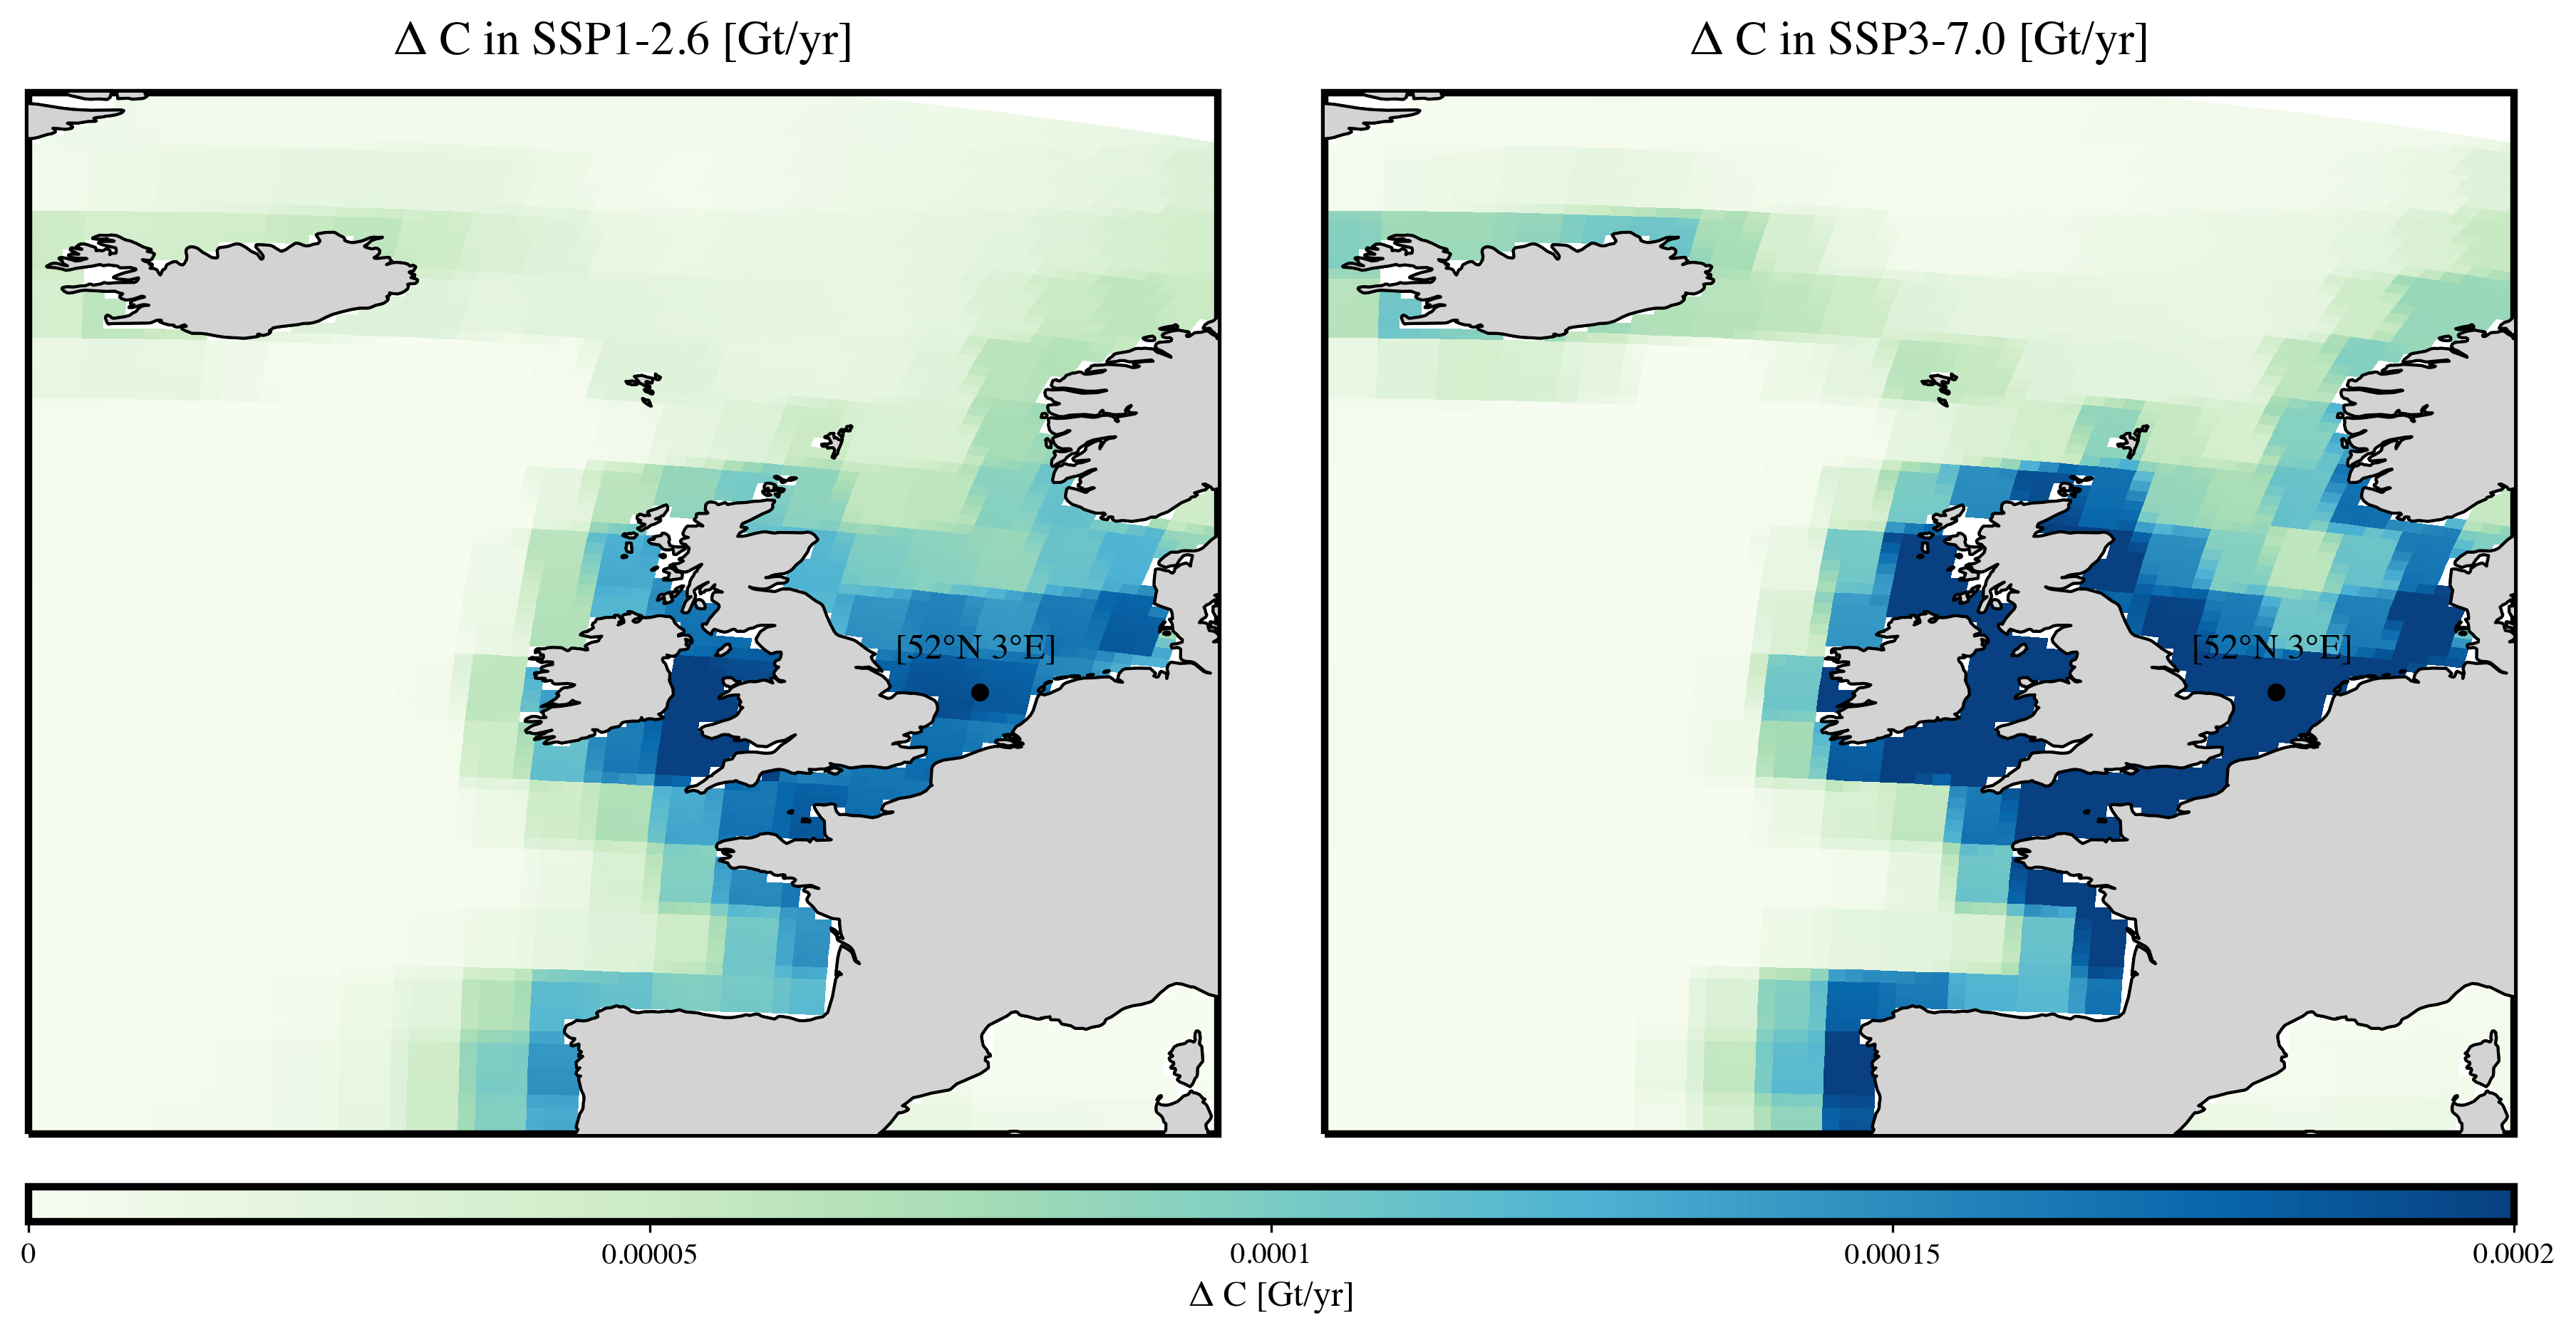
\includegraphics[width=15cm]{fig/3_Results/CO2flux/Cgt.png}

\end{figure}

In order to determine the magnitude of \ac{oae} impacts on the \ch{CO2} flux in European waters, the baseline-to-\ac{oae} change in carbon inventory in Gt yr\textsuperscript{-1} averaged over the last simulation decade was plotted (\cref{cgt}). It was found that \ac{oae} implementation has an additional uptake potential of 0.1779 GtC yr\textsuperscript{-1} in SSP1-2.6, which increases to 0.24 GtC yr\textsuperscript{-1} in SSP3-7.0. Following the definition in \cite{NAP26278}, where medium-to-high potential is set to a minimum threshold of 0.1–1.0 Gt \ch{CO2} yr\textsuperscript{-1}, these results confirm that \ac{oae} is expected to become an efficient tool for climate mitigation and reach net negative emissions. Additionally, the maps show that the southern North Sea offers an ideal location for \ac{oae} testing and similar regions should be viewed as the primary targets. 

\newpage\cleardoublepage
\chapter{Discussion:}

The results presented in the previous section confirm the potential of \ac{oae} to lower ocean \ch{pCO2} and enhance the downward \ch{CO2} flux in European waters, as well as the additional benefit of increasing seawater pH and mitigating future ocean acidification. Seasonally, \ac{oae} impacts resulted in the dampening of the ocean \ch{pCO2} monthly cycle and in the amplification of the \ch{CO2} flux cycle, as hypothesised in the first chapter. Lastly, the change in carbon inventory that is observed in \cref{cgt} highlights \ac{oae} as a suitable candidate for achieving the \ac{pa}. Below, an in-depth analysis of the causes that may trigger such system changes are presented. 

\section[\texorpdfstring{OAE}{OAE} impacts at the European average:]{\ac{oae} impacts at the European average:}

All maps show that system perturbations for all variables happen within the model domain, in the proximity of the injection site, and the signal does not propagate far by the end of the century. This leads to conclude that \ac{oae} deployment is spatially limited to where alkalinity is added, at least for the upper 50 metres of the ocean surface. Such outcome is corroborated by a recent experiment carried out by \cite{wang2023simulated}. 

Open-ocean regions like Iceland, Norway and Spain show few-to-absent perturbations with alkalinity addition. The most affected region is the North Sea, and especially the southern North Sea, which delivers pronounced system alterations. In addition to the fact that this is the location where the experiment is simulated, the shallower, well-mixed ocean system allows for alkalinity to accumulate at the surface and to not be lost due to mixing-induced subduction before equilibration is completed \citep{wang2023simulated}. Ocean \ch{pCO2} seasonal amplification at high latitudes diverges from the expected outcome and may be the result of \ac{dic}-driven modulations. 

In SSP1-2.6, both the baseline and the \ac{oae} scenario register higher alkalinity values than their respective SSP3-7.0 levels. This may be the result of multiple mechanisms influencing alkalinity fluxes and corresponding sources and sinks. In the case of \ac{foci}, nutrient consumption and supply or variations of the carbonate counter pump may explain such deviations. 

When observing the seasonal trend of alkalinity in both SSP1-2.6 and SSP3-7.0, a reversed pattern is detected (A and C of \cref{alkalinity}), especially at the very first ocean layer (right graph of \cref{EUalkalinitysurface}). In the baseline, alkalinity values progressively grow with depth. Seasonally, this translates in maxima registered in winter, when stronger winds force surface water mixing with the deeper, more alkalinised subsurface. Minima are then detected in summer, when \ac{sst} increases and enhanced ocean stratification prevents mixing. 

When alkalinity is added to the surface layer, as it is the case of the simulation experiments, a system shift is visible. Alkalinity is high at the top layer and progressively lowers with depth, up to about 100 metres, where an ascending trajectory is restored (left graph of \cref{EUalkalinitysurface}). Winter mixing results in the surface water being incorporated with the less alkalinised subsurface region, whereas summer stratification leaves alkalinity-rich water at the top.

In both SSP1-2.6 and SSP3-7.0, \ch{pCO2} minima are registered in spring, which may be the result of phytoplankton bloom and consequent high photosynthetic activity, where \ch{CO2} is consumed. In SSP3-7.0, major atmospheric \ch{CO2} emissions force \ch{pCO2} to rise progressively until the end of the simulations, even with alkalinity enhancement (not shown). Ocean \ch{pCO2} seasonal amplitude is reduced due to the fact that an alkalinised ocean minimises \ch{pCO2} sensitivity to \ac{dic} changes, described by \ch{CO2} fluxes.

From these results, it is assumed that \ac{rf} lowers in the study region, as seawater buffering capacity is enhanced. This system shift is expressed by the fact that larger \ac{dic} variations are needed to produce the same \ch{pCO2} alterations that would be realised in a non-alkalinised ocean \citep{schwinger2022report}. Hence, it is likely \ch{pCO2} sensitivity to its seasonal drivers, rather than the drivers themselves, the cause of this regime shift, as cited in \cite{lerner2021drivers}.

In accordance with previous estimates \citep{schwinger2022report}, \ac{oae} causes an amplification of the \ch{CO2} seasonal flux for both \ac{ssp}s. \ac{oae} enlarges the air-to-sea disequilibrium, which then requires higher \ch{CO2} input to be restored. In all scenarios, highest levels of alkalinity are recorded between the end of summer and the onset of autumn but largest uptake takes place in winter, therefore introducing a short response lag due to re-equilibration timescales. In the \ac{oae} scenario, alkalinity addition forces a greater \ch{CO2} flux downward in wintertime, meaning that \ac{oae} induces an asymmetrical shift of the ocean regime, with much lower lows than lower highs.

Such stronger \ch{CO2} downward movement in both scenarios takes the form of an increment of the \ac{dic} pool. Highest peaks are in spring and lowest in autumn, consistent with an expected requilibration lag, as greatest uptake happens in winter months. For the same relation expressed above by \ac{rf}, in an alkalinised ocean, larger variations in the \ac{dic} pool elicit the same change in the ocean \ch{pCO2}. However, although maintaining a similar cycle compared to the baseline, \ac{dic} seasonal amplitude is slightly decreased with alkalinity addition, so that a relation between alkalinity and \ac{dic} seasonal compression seems to take place (A and B of \cref{alkalinity} and \cref{dic}).  

As predicted, \ac{oae} allows for a pH increase by favouring a shift towards a carbonate-dominated system. With \ac{oae}, ocean acidification is therefore mitigated. Largest baseline-to-\ac{oae} anomaly is recorded in summer, reproducing most pronounced \ac{oae} impacts at the corresponding highest seasonal acidification phase. This translates in a compression of the pH seasonal cycle, also probably due to the fact that \ch{H+} annual concentration grows faster than its seasonal increase \citep{kwiatkowski2022modified, kwiatkowski2018diverging}.

\section[\texorpdfstring{OAE}{OAE} impacts at location S:]{\ac{oae} impacts at location S:}

In the southern North Sea, \ch{CO2} flux modulations are dominated by temperature changes (see B of \cref{dsmw}) \citep{rodgers2023seasonal, salt2013variability, prowe2009mechanisms}, resulting in \ac{dic} minima being observed in summer (at highest \ch{pCO2}), when warm temperatures elicit outgassing, and in ocean \ch{pCO2} maxima being registered in winter, at highest gas solubility. Additionally, a much larger flux change is reflected in comparison to the European average. In SSP1-2.6, \ch{CO2} seasonal amplitude doubles and, in SSP3-7.0, it triples, in accordance with \cite{lenton2018assessing} who found greater net uptake under greater atmospheric \ch{CO2} concentration. In both scenarios, the system change is asymmetrical, detecting much lower lows than lower highs (F and H of \cref{co2flux}). 

Air-sea re-equilibration can take from a few months to even years to complete, depending on physical properties such as latitude, air-sea gas exchange, \ac{mld}, water mixing and wind speed \citep{jones2014spatial}. Therefore, drawing from \cite{wang2023simulated} and \cite{jones2014spatial}, it is deduced that the shallower, well-mixed waters of the southern North Sea encourage fast re-equilibration, which trumps mean water residence time and allows for efficient carbon sequestration. Quantifying such temporal gaps between system forcing and air-sea exchange is of paramount importance when addressing \ac{oae} potential, as incomplete requilibration could substantially inhibit \ac{oae} efficiency \citep{wang2023simulated, jones2014spatial}. 

\ch{pCO2} levels plummet, with lowest registered values being 114 µatm at SSP1-2.6 and 277 µatm at SSP3-7.0. Differently from the European average, the thermal component drives seasonality at location S, and minima are registered in winter, at highest seawater solubility. In analogy with \cite{fassbender2018seasonal}, $\Delta$ \ch{pCO2} is highest in the season where the associated seasonal driver operates to reduce the ocean \ch{CO2} sink potential. In this case, $\Delta$ \ch{pCO2} increases in summer, when rising temperatures force a reduced gas solubility and inhibit ocean uptake. \ac{oae} is therefore most efficient during that phase \citep{fassbender2018seasonal}. 

\ac{dic} absolute values are considerably greater than at the European average, reaching 2450 mmol m\textsuperscript{-3} in SSP1-2.6 and 2738 mmol m\textsuperscript{-3} in SSP3-7.0. As expected, the seasonal amplitude is enhanced, especially under the higher-emission scenario, since an alkalinised ocean induces a larger \ac{dic} seasonal cycle to modulate the same \ch{pCO2} response. Larger \ac{dic} variance in SSP3-7.0 means that the ocean buffering capacity is lower, as confirmed by \cite{lenton2018assessing}. This response is likely due to the enhanced seasonal cycle of alkalinity observed in E and G of \cref{alkalinity}, where alkalinity regulates \ac{dic} seasonality, and to higher atmospheric \ch{CO2} concentration, which creates a larger disequilibrium to be restored.  

pH seasonal amplitude remains fundamentally unchanged. Based on previous research, this leads to believe that, with alkalinity enhancement, the annual \ch{H+} concentration rises proportionally to its seasonal fluxes. Under a higher emission scenario, $\Delta$ pH absolute values are lower, meaning that, unlike all other variables where \ac{oae}-induced modulations are highest in SSP3-7.0, alkalinity enhancement is not as effective in bringing about the same mitigating effect to acidification with elevated atmospheric \ch{CO2}. This is corroborated by \cite{lenton2018assessing}, where it was observed that acidification is relieved more efficiently under a lower emission scenario.  
\newpage\cleardoublepage
\chapter{Considerations for future research:}

The present analysis aimed to understand the imposed impacts of \ac{oae} on the seasonal cycle of \ch{CO2} flux and ocean \ch{pCO2} in European waters, and how such changes vary depending on the future background climate. Given the knowledge vacuum present in current literature, these results were able to provide an in-depth representation of the mechanisms triggered by \ac{oae}, together with a freely accessible GitHub repository that supports open-source research. Although defining precise interpretations on the observed system changes is beyond the scope of this study, the results presented above can help formulate some key conclusions for future investigation. 

To answer the first research question addressing the impacts of \ac{oae} on the seasonal cycle of ocean \ch{pCO2} and \ch{CO2} flux, \ac{oae} encourages a compression of the former and an amplification of the latter. Secondly, to explain the causes and effects of such variations, it can be concluded that the ocean \ch{pCO2} compression is the result of its reduced sensitivity to \ac{dic} inputs. This mechanism allows for a greater \ch{CO2} modulation given by the larger air-to-sea gas disequilibrium, hence the \ch{CO2} amplification pattern. Lastly, the higher climate background state (SSP3-7.0) forces a magnification of the aforementioned \ac{oae}-induced effects. Alkalinity and \ac{dic} variations are also more pronounced under SSP3-7.0, although ocean acidification is mitigated more efficiently under SSP1-2.6. 

Drawing from this study's results, theoretical assumptions can be made on both the ideal location and the desirable time to perform \ac{oae}. From existing literature, it is established that fast air-sea re-equilibration happens in conditions of shallow \ac{mld} and strong wind-driven mixing \citep{jones2014spatial}. Geographically, regions like the southern North Sea represent a favourable location as they display a shallow water column, which impedes alkalinity loss to the subsurface, and which, especially in wintertime, undergo strong wind-induced mixing, speeding up the adjustment.

Due to the asymmetrical uptake change that \ac{oae} generated in the experiments, and assuming two to three-month equilibration rate in areas like the southern North Sea, the best time to perform \ac{oae} would be in the season previous to the phase that already produces highest ocean \ch{CO2} uptake. Taking the southern North Sea as an example, alkalinity should be added in autumn to allow for full equilibration over winter and maximise \ac{oae} potential. This conclusion, however, disagrees with \cite{lenton2018assessing}, who did not observe any seasonally-dependent efficiency. 

Given these conclusions, some limitations and recommendations for future research can be discussed. Firstly, although the European coastline accommodates multiple river mouths, riverine inputs of alkalinity are not resolved in \ac{foci}. This creates a vacuum for generating realistic data on alkalinity and on its dependent variables. Likewise, coastal sediment biogeochemistry is poorly resolved in the model, although alkalinity generation from the anaerobic degradation of \ac{om} is a major process that regulates seasonality in the region of focus \citep{thomas2009enhanced}. It would therefore be valuable to integrate these components in the model and assess more realistic data for future scientific assumptions. 

In past literature \citep{schwinger2022report, fassbender2022quantifying}, \ch{CO2} seasonality was investigated by separating the thermal (\ac{sst}) from the non-thermal (\ac{dic}) component. The same approach could be applied in this case to weigh the relative impact of each on the seasonal \ch{CO2} cycle. Additionally, it is well established that seasonal \ch{CO2} fluxes are influenced by, among others, wind speed \citep{jones2014spatial} and \ac{mld} \citep{jo2022future, jones2014spatial}. Evaluating the part that these components play in regulating the seasonality of \ch{CO2} would therefore benefit the present study and give insight on the possible loops triggered by \ac{oae} application.

Moreover, as this analysis is carried out for the first 50 metres of the ocean surface, it is not possible to see where accumulated \ac{dic} travels beyond this threshold. Investigating the pathway that \ac{dic} would take and whether, for example, it would spread far from where it sinks or whether it would resurface and be respired beyond the model domain are all relevant assumptions that should be tested. On this note, given the influence of the \ac{mld} in the seasonal carbon cycle, replacing the 50-metre threshold with the calculated \ac{mld} (of which a \ac{foci} variable already exists) would better describe water transport as a region of uniform mixing. 

Regarding the features of this study's experiments, they cover only one of the many ways in which \ac{oae} could be implemented. Other, practically easier schemes are already under investigation: addition performed in seasonal pulses, rather than continuously, or at defined point sources such as river mouths, rather than along an entire coastline. Different application simulations can help understand under which conditions alkalinity enhancement is most effective.

In conclusion, this study contributed to shed light on the impacts of \ac{oae} on the carbon cycle by analysing its seasonal fluxes. As climate change forces global temperatures to rise, the ocean will likely suffer from a more precarious equilibrium and will be more vulnerable to thermally-driven changes. With the theoretical potential of \ac{oae} to alleviate climate warming, further investigation is encouraged and may create the premises for conscious large-scale application. \newpage\cleardoublepage

\bibliographystyle{apsr}

\chapter*{Bibliography}
\addcontentsline{toc}{chapter}{Bibliography}
\bibliography{bib/bib_final}

\end{document}